%% abtex2-modelo-trabalho-academico.tex, v-1.9.7 laurocesar
%% Copyright 2012-2019 by abnTeX2 group at http://www.abntex.net.br/ 
%%
%% This work may be distributed and/or modified under the
%% conditions of the LaTeX Project Public License, either version 1.3
%% of this license or (at your option) any later version.
%% The latest version of this license is in
%%   http://www.latex-project.org/lppl.txt
%% and version 1.3 or later is part of all distributions of LaTeX
%% version 2005/12/01 or later.
%%
%% This work has the LPPL maintenance status `maintained'.
%% 
%% The Current Maintainer of this work is the abnTeX2 team, led
%% by Lauro César Araujo. Further information are available on 
%% http://www.abntex.net.br/
%%
%% This work consists of the files abntex2-modelo-trabalho-academico.tex,
%% abntex2-modelo-include-comandos and abntex2-modelo-references.bib
%%

% ------------------------------------------------------------------------
% ------------------------------------------------------------------------
% abnTeX2: Modelo de Trabalho Academico (tese de doutorado, dissertacao de
% mestrado e trabalhos monograficos em geral) em conformidade com 
% ABNT NBR 14724:2011: Informacao e documentacao - Trabalhos academicos -
% Apresentacao
% ------------------------------------------------------------------------
% ------------------------------------------------------------------------

\documentclass[
	% -- opções da classe memoir --
	12pt,				% tamanho da fonte
	openright,			% capítulos começam em pág ímpar (insere página vazia caso preciso)
	twoside,			% para impressão em recto e verso. Oposto a oneside
	a4paper,			% tamanho do papel. 
	% -- opções da classe abntex2 --
	%chapter=TITLE,		% títulos de capítulos convertidos em letras maiúsculas
	%section=TITLE,		% títulos de seções convertidos em letras maiúsculas
	%subsection=TITLE,	% títulos de subseções convertidos em letras maiúsculas
	%subsubsection=TITLE,% títulos de subsubseções convertidos em letras maiúsculas
	% -- opções do pacote babel --
	english,			% idioma adicional para hifenização
	french,				% idioma adicional para hifenização
	spanish,			% idioma adicional para hifenização
	brazil				% o último idioma é o principal do documento
	]{abntex2}

% ---
% Pacotes básicos 
% ---
\usepackage{lmodern}			% Usa a fonte Latin Modern			
\usepackage[T1]{fontenc}		% Selecao de codigos de fonte.
\usepackage[utf8]{inputenc}		% Codificacao do documento (conversão automática dos acentos)
\usepackage{indentfirst}		% Indenta o primeiro parágrafo de cada seção.
\usepackage{color}				% Controle das cores
\usepackage{graphicx}			% Inclusão de gráficos
\usepackage{microtype} 			% para melhorias de justificação
 \usepackage{pdfpages}          % Incluir os pdfs necessários
% ---
		
% ---
% Pacotes adicionais, usados apenas no âmbito do Modelo Canônico do abnteX2
% ---
%\usepackage{lipsum}				% para geração de dummy text
\usepackage{pdflscape}
\usepackage{multirow}
\usepackage{amsmath}
\usepackage{amsfonts}
\usepackage{mathtools}
\usepackage{fixltx2e}
%\usepackage[super,sort&compress,comma]{natbib} 
\usepackage{setspace}
%\usepackage{geometry}
\usepackage{nicefrac}
\usepackage{notoccite}
\usepackage[section]{placeins}


% ---
%\renewcommand{\cleardoublepage}{\newpage}
\newcommand\mat[1]{\mathcal{#1}}
\graphicspath{{images/}}

% ---
% Pacotes de citações
% ---
\usepackage[brazilian,hyperpageref]{backref}	 % Paginas com as citações na bibl
\usepackage[num,abnt-etal-text=emph, abnt-emphasize=bf]{abntex2cite}	% Citações padrão ABNT
\citebrackets[] % use [REF]
%\usepackage[alf]{abntex2cite}	% Citações padrão ABNT

% --- 
% CONFIGURAÇÕES DE PACOTES
% --- 

% ---
% Configurações do pacote backref
% Usado sem a opção hyperpageref de backref
\renewcommand{\backrefpagesname}{Citado na(s) página(s):~}
% Texto padrão antes do número das páginas
\renewcommand{\backref}{}
% Define os textos da citação
\renewcommand*{\backrefalt}[4]{
	\ifcase #1 %
		Nenhuma citação no texto.%
	\or
		Citado na página #2.%
	\else
		Citado #1 vezes nas páginas #2.%
	\fi}%
% ---

% ---
% Informações de dados para CAPA e FOLHA DE ROSTO
% ---
\titulo{Validação do campo de força 2016H66 para a simulação de dendrímeros PAMAM e PPI. Um estudo sistemático dos efeitos da geração e do pH}
\autor{Mayk Caldas Ramos}
\local{Brasil}
\data{Fevereiro/2019}
\orientador{Bruno Araujo Cautiero Horta}
\coorientador{}
\instituicao{%
  Universidade Federal do Rio de Janeiro -- UFRJ
  \par
  Instituto de Química
  \par
  Programa de Pós-Graduação em Química}
\tipotrabalho{Dissertação de Mestrado}
% O preambulo deve conter o tipo do trabalho, o objetivo, 
% o nome da instituição e a área de concentração 
\preambulo{Dissertação apresentada ao Programa de Pós-Graduação em Química, PGQU, da Universidade Federal Do Rio de Janeiro, como parte dos requisitos necessários à obtenção do título de Mestre em Ciências (Química).}
% ---


% ---
% Configurações de aparência do PDF final

% alterando o aspecto da cor azul
\definecolor{blue}{RGB}{41,5,195}

% informações do PDF
\makeatletter
\hypersetup{
     	%pagebackref=true,
		pdftitle={\@title}, 
		pdfauthor={\@author},
    	pdfsubject={\imprimirpreambulo},
	    pdfcreator={Mayk Caldas Ramos},
		pdfkeywords={Dendrímeros}{PAMAM}{PPI}{Dinâmica Molecular}{}, 
		colorlinks=true,       		% false: boxed links; true: colored links
    	linkcolor=blue,          	% color of internal links
    	citecolor=blue,        		% color of links to bibliography
    	filecolor=magenta,      		% color of file links
		urlcolor=blue,
		bookmarksdepth=4
}
\makeatother
% --- 

% --- 
% Espaçamentos entre linhas e parágrafos 
% --- 

% O tamanho do parágrafo é dado por:
\setlength{\parindent}{1.3cm}

% Controle do espaçamento entre um parágrafo e outro:
\setlength{\parskip}{0.2cm}  % tente também \onelineskip

% ---
% compila o indice
% ---
\makeindex
% ---

% ----
% Início do documento
% ----

%%% -----
%%% Formato de cabeçalho/rodapé romano nos elementos pré-textuais
%%% -----

%% Novo estilo
\makepagestyle{estilo_pretextual} %%% escolha um nome
  \makeevenhead{estilo_pretextual}{}{}{\ABNTEXfontereduzida \textbf \thepage}
  \makeoddhead{estilo_pretextual}{}{}{\ABNTEXfontereduzida \textbf \thepage}

%% Customiza comando \pretextual
\renewcommand{\pretextual}{
  \pagenumbering{roman} %%% ou \pagenumbering{Roman}
  \aliaspagestyle{chapter}{estilo_pretextual}% customizing chapter pagestyle
  \pagestyle{estilo_pretextual}
  \aliaspagestyle{cleared}{empty}
  \aliaspagestyle{part}{estilo_pretextual}
}

% ---
% Ajusta a marca \textual para que a numeração volte a ser arábica
% nos elementos textuais
\let\oldtextual\textual        % copia o comando \textual anterior para \oldtextual
\renewcommand{\textual}{%
  \oldtextual%
  \pagenumbering{arabic} % volta à numeração arábica
}
% ---

\begin{document}

% Seleciona o idioma do documento (conforme pacotes do babel)
%\selectlanguage{english}
\selectlanguage{brazil}

% Retira espaço extra obsoleto entre as frases.
\frenchspacing 

% ----------------------------------------------------------
% ELEMENTOS PRÉ-TEXTUAIS
% ----------------------------------------------------------
% \pretextual

% ---
% Capa
% ---
%\imprimircapa

% ---
% Capa
% ---
  \begin{capa}
  
   \thispagestyle{plain}
 
   
   \begin{center}
      
  \imprimirinstituicao
  
  \end{center}
  
  \vspace*{\fill}
  
  \begin{center}
  
  \Large\imprimirtitulo
  
  \end{center}
  
  \vspace*{\fill}
  
  \begin{center}
  
  \imprimirautor
  
  \end{center}
  
  \vspace*{\fill}
  
  \begin{center}
  
  \imprimirlocal
  
  \end{center}
  
   \begin{center}
  
  \imprimirdata
  
  \end{center}

  \end{capa}


% ---

% ---
% Folha de rosto
% (o * indica que haverá a ficha bibliográfica)
% ---
\imprimirfolhaderosto*
% ---

% ---
% Inserir a ficha bibliografica
% ---

% Isto é um exemplo de Ficha Catalográfica, ou ``Dados internacionais de
% catalogação-na-publicação''. Você pode utilizar este modelo como referência. 
% Porém, provavelmente a biblioteca da sua universidade lhe fornecerá um PDF
% com a ficha catalográfica definitiva após a defesa do trabalho. Quando estiver
% com o documento, salve-o como PDF no diretório do seu projeto e substitua todo
% o conteúdo de implementação deste arquivo pelo comando abaixo:
%
 \begin{fichacatalografica}
     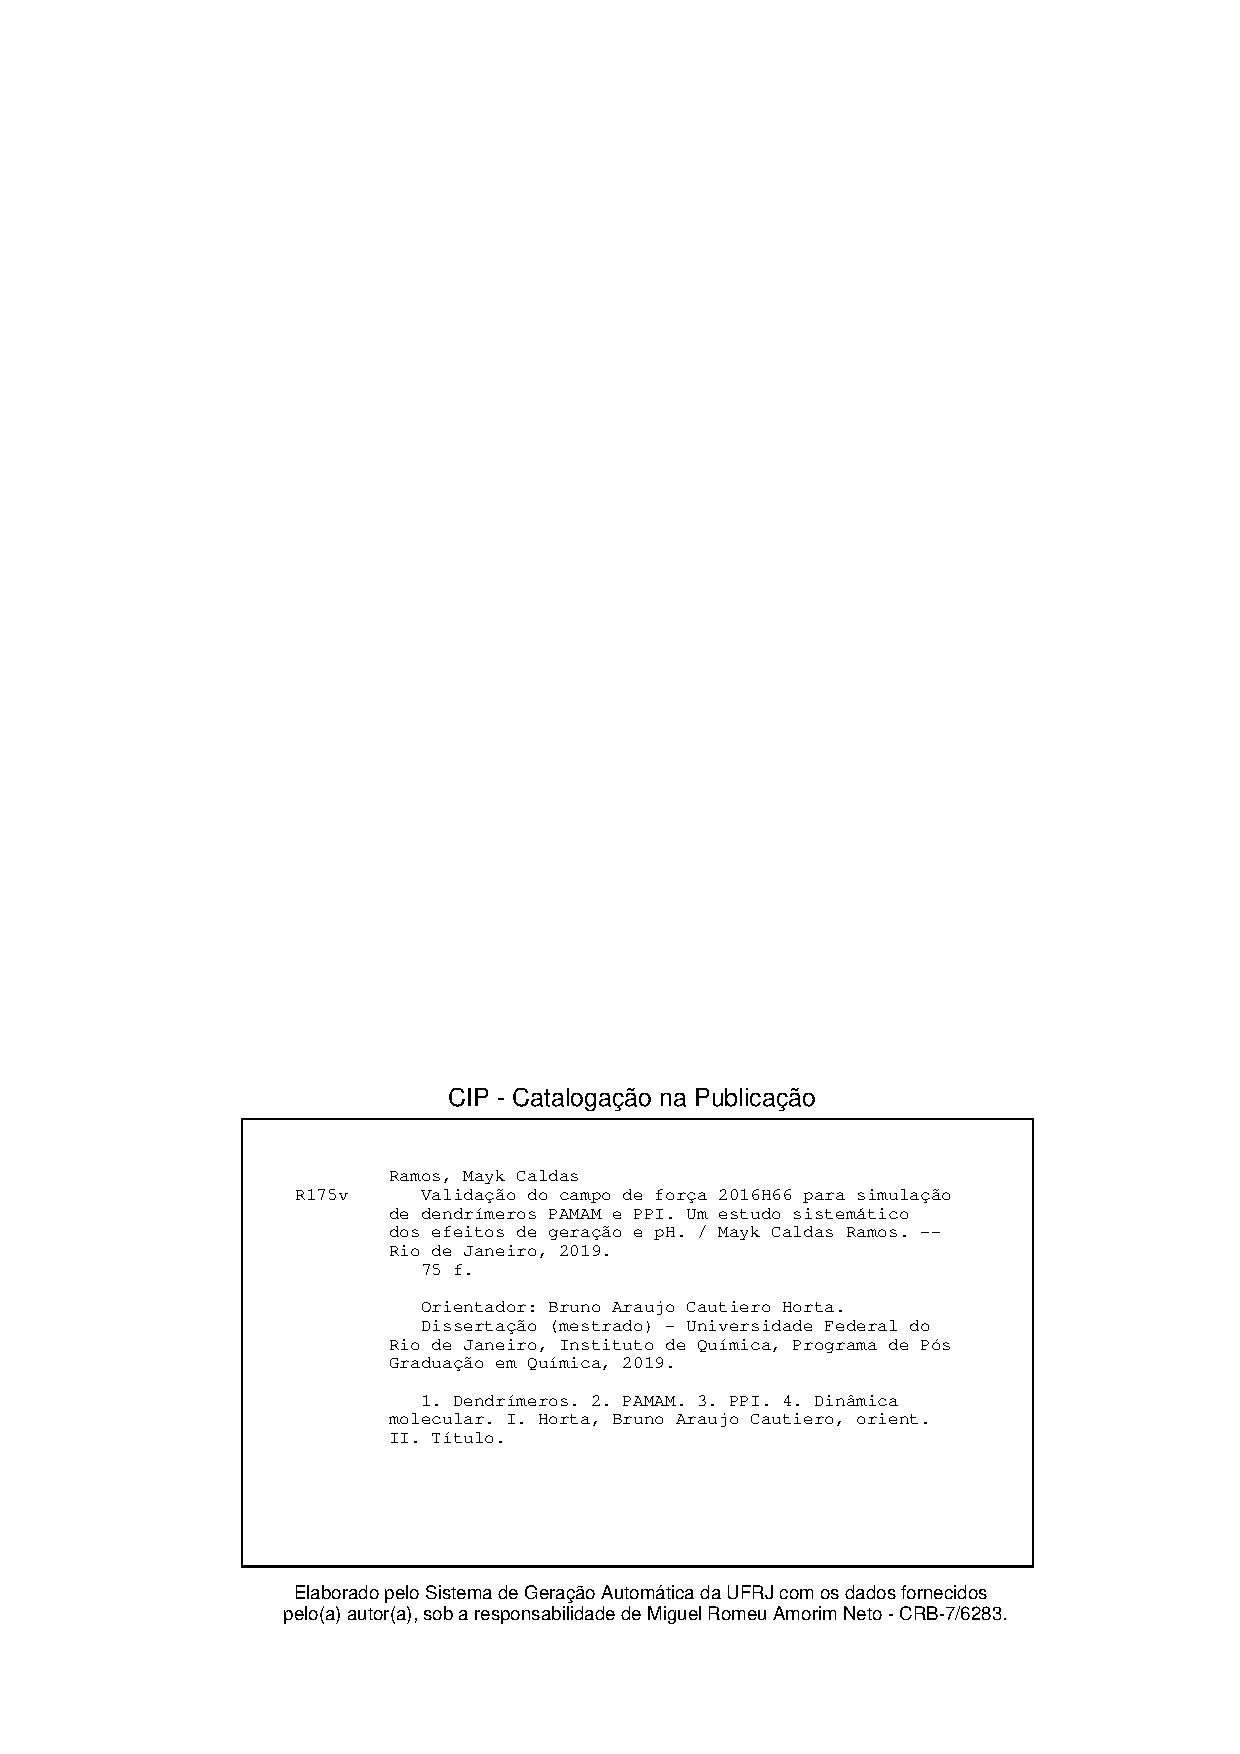
\includepdf{fichaCatalog.pdf}
 \end{fichacatalografica}

% \begin{fichacatalografica}
% 	\sffamily
% 	\vspace*{\fill}					% Posição vertical
% 	\begin{center}					% Minipage Centralizado
% 	\fbox{\begin{minipage}[c][8cm]{13.5cm}		% Largura
% 	\small
% 	\imprimirautor
% 	%Sobrenome, Nome do autor
	
% 	\hspace{0.5cm} \imprimirtitulo  / \imprimirautor. --
% 	\imprimirlocal, \imprimirdata-
	
% 	\hspace{0.5cm} \thelastpage p. : il. (algumas color.) ; 30 cm.\\
	
% 	\hspace{0.5cm} \imprimirorientadorRotulo~\imprimirorientador\\
	
% 	\hspace{0.5cm}
% 	\parbox[t]{\textwidth}{\imprimirtipotrabalho~--~\imprimirinstituicao,
% 	\imprimirdata.}\\
	
% 	\hspace{0.5cm}
% 		1. Dendrímeros.
% 		2. PAMAM.
% 		3. PPI.
% 		4. Dinâmica Molecular.
% 		I. Bruno Araújo Cautiero Horta.
% 		II. Universidade Federal do Rio de Janeiro.
% 		III. Programa de Pós-Graduação em Química.
% 		IV. Título 			
% 	\end{minipage}}
% 	\end{center}
%\end{fichacatalografica}
% ---

% ---
% Inserir errata
% ---
%\begin{errata}
%Elemento opcional da \citeonline[4.2.1.2]{NBR14724:2011}. Exemplo:
%
%\vspace{\onelineskip}
%
%FERRIGNO, C. R. A. \textbf{Tratamento de neoplasias ósseas apendiculares com
%reimplantação de enxerto ósseo autólogo autoclavado associado ao plasma
%rico em plaquetas}: estudo crítico na cirurgia de preservação de membro em
%cães. 2011. 128 f. Tese (Livre-Docência) - Faculdade de Medicina Veterinária e
%Zootecnia, Universidade de São Paulo, São Paulo, 2011.
%
%\begin{table}[htb]
%\center
%\footnotesize
%\begin{tabular}{|p{1.4cm}|p{1cm}|p{3cm}|p{3cm}|}
%  \hline
%   \textbf{Folha} & \textbf{Linha}  & \textbf{Onde se lê}  & \textbf{Leia-se}  \\
%    \hline
%    1 & 10 & auto-conclavo & autoconclavo\\
%   \hline
%\end{tabular}
%\end{table}
%
%\end{errata}
% ---

% ---
% Inserir folha de aprovação
% ---

% Isto é um exemplo de Folha de aprovação, elemento obrigatório da NBR
% 14724/2011 (seção 4.2.1.3). Você pode utilizar este modelo até a aprovação
% do trabalho. Após isso, substitua todo o conteúdo deste arquivo por uma
% imagem da página assinada pela banca com o comando abaixo:
%
\begin{folhadeaprovacao}
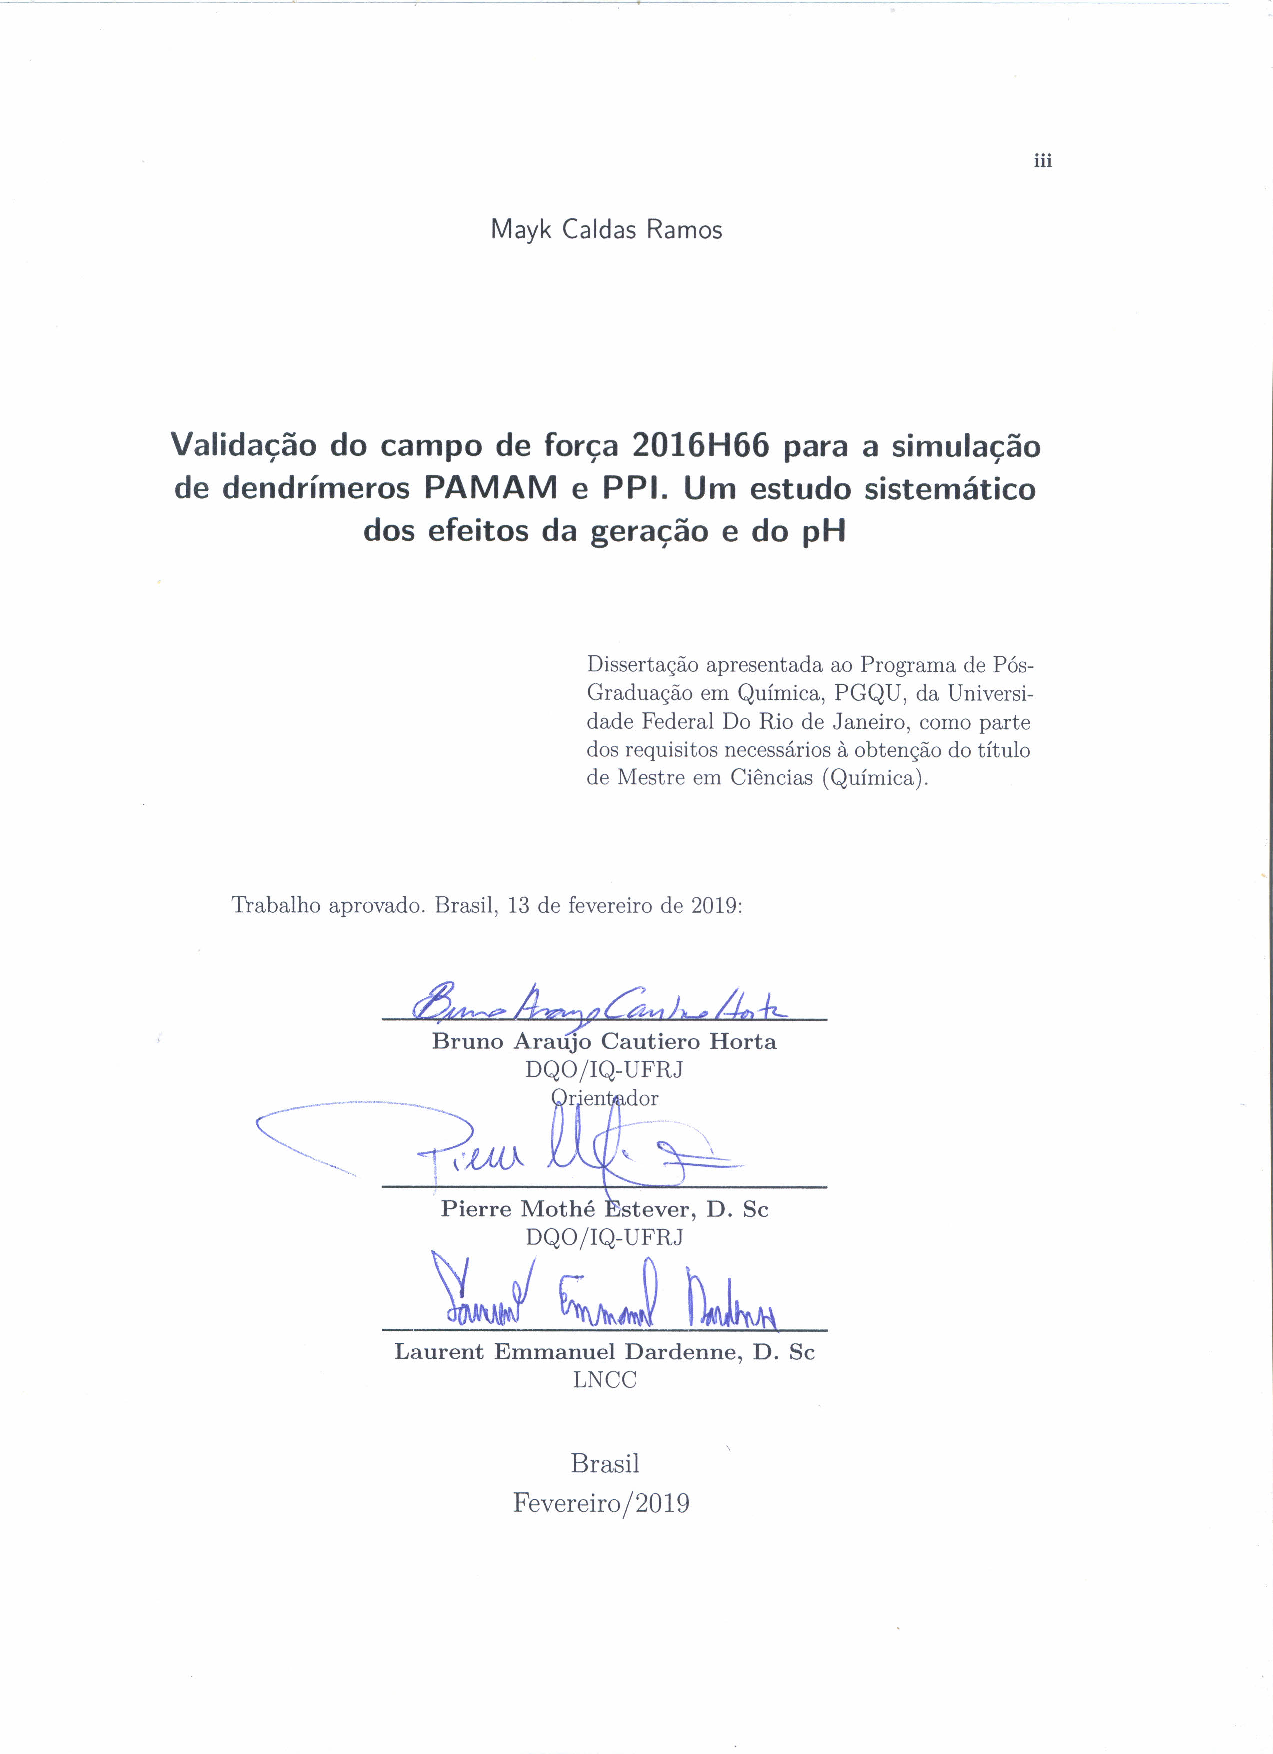
\includepdf{fichaAprov.pdf}
\end{folhadeaprovacao}
%
% \begin{folhadeaprovacao}

%   \begin{center}
%     {\ABNTEXchapterfont\large\imprimirautor}

%     \vspace*{\fill}\vspace*{\fill}
%     \begin{center}
%       \ABNTEXchapterfont\bfseries\Large\imprimirtitulo
%     \end{center}
%     \vspace*{\fill}
    
%     \hspace{.45\textwidth}
%     \begin{minipage}{.5\textwidth}
%         \imprimirpreambulo
%     \end{minipage}%
%     \vspace*{\fill}
%   \end{center}
        
%   Trabalho aprovado. \imprimirlocal, 13 de fevereiro de 2019:

%   \assinatura{\textbf{\imprimirorientador} \\ DQO/IQ-UFRJ \\ Orientador} 
%   \assinatura{\textbf{Pierre Mothé Estever, D. Sc} \\ DQO/IQ-UFRJ}
%   %\assinatura{\textbf{Thiago Messias Cardozo, D. Sc} \\ DFQ/IQ-UFRJ}
%   \assinatura{\textbf{Laurent Emmanuel Dardenne, D. Sc} \\ LNCC}
%   %\assinatura{\textbf{Ernesto Raúl Caffarena, D. Sc} \\ Fiocruz}

%   \begin{center}
%     \vspace*{0.5cm}
%     {\large\imprimirlocal}
%     \par
%     {\large\imprimirdata}
%     \vspace*{1cm}
%   \end{center}
  
% \end{folhadeaprovacao}
% ---

% ---
% Dedicatória
% ---
\begin{dedicatoria}
   \vspace*{\fill}
   \centering
   \noindent
   \textit{ À todos que, de alguma forma, tornaram esse trabalho possível. } \vspace*{\fill}
\end{dedicatoria}
% ---

% ---
% Agradecimentos
% ---
\begin{agradecimentos}

Primeiramente, gostaria de agradecer à minha família pelo suporte até aqui. Pela força em aceitar que eu seguiria por mais tempo na minha carreira acadêmica e não partir por um caminho empresarial, pelo apoio quando não fui à reuniões de família pela necessidade de estudar e por eventuais suportes financeiros quando necessário. Muito Obrigado!

Aos poucos amigos que trouxe desde a juventude e que, quando a quântica e a estatística não fizeram mais sentido, sempre estiveram aqui pra uma conversa e uma cerveja. Seguimos juntos mesmo eu estando sumido.

Ao meu orientador, por entender as vezes que eu sumia do laboratório por preguiça de sair nesse calor e querer trabalhar de casa, por me chamar de volta pro lab pra que eu interagisse com o grupo, pelas mensagens motivadoras, pelo crescimento pessoal além do científico e por tudo mais até aqui. Valeu!

Aos colegas do laboratório LabMMol, ciência é feita de pessoas e discussões, mesmo que pareçam absurdas à uma primeira visão. Espero ainda encontrar vocês por aí.

Ao grupo que passei de penetra à quase membro. Desculpe qualquer piada desnecessária e obrigado pelas discussões. Cthulhu Fhtagn.

Ao grupo de quarta, que ainda não foi decidido se é um grupo quatro estrelas ou de quarta categoria, mas as conversas, risadas, discussões e brincadeiras foram de vital importância para a realização de um ócio criativo bem feito. Um brinde!

A todos os professores da UFRJ com os quais interagi, obrigado pelas noites de sono não dormidas, seja por uma prova na semana seguinte ou por virar a noite estudando uma curiosidade pessoal causada por vocês.

Agradeço, também, ao Lobo Carneiro (Loboc) e ao Núcleo de Atendimento a Computação de Alto Desempenho (Nacad) pela capacidade de computação sem a qual esse estudo não seria terminado e à Capes e à Faperj pela bolsa de mestrado e o financiamento do projeto, respectivamente, sem os quais esse estudo também não seria possível.

Abraço!


\end{agradecimentos}
% ---

% ---
% Epígrafe
% ---
\begin{epigrafe}
    \vspace*{\fill}
	\begin{flushright}
		\textit{``Study hard what interests you the most in the most undisciplined,\\
		irreverent and original manner possible.''}\\
		(Richard P. Feynmann)
		
		%\textit{``Science has not yet taught us if madness is or is not the sublimity of the intelligence.''}\\
        %(Edgar Allan Poe)
        
        \textit{``The oldest and strongest emotion of mankind is fear, \\
        and the oldest and strongest kind of fear is fear of the unknown.''}\\
        (H. P. Lovecraft)
        
        %\textit{``When asked, `How do you write?' I invariably answer, `one word at a time.' ''}\\
        %(Stephen King)
        
        \textit{``All we are is dust in the wind''}\\
        (Kansas)
        
        %\textit{``I find it hard to tell you 'cause I find it hard to take. When people run in circles it's a very, very mad world.''}\\
        %(Tears for Fears)
        
	\end{flushright}
\end{epigrafe}
% ---

% ---
% RESUMOS
% ---

% resumo em português
\setlength{\absparsep}{18pt} % ajusta o espaçamento dos parágrafos do resumo
\begin{resumo}
Dendrímeros são macromoléculas sintéticas cuja estrutura é baseada em blocos de construção bem definidos que são repetidos de maneira sistemática.
Em sua síntese, um bloco nuclear é considerado e, a partir dele, blocos intermediários são conectados.
A cada camada radial de blocos intermediários utilizados, dizemos que sua geração aumentou em uma unidade.
Portanto, a geração é utilizada para referenciar o tamanho do dendrímero.
Ao se alcançar o tamanho desejado, uma camada de blocos terminais é adicionada.
Por ser uma molécula sintética, sua versatilidade em aplicações de interesse só se limita pela criatividade do pesquisador.
A estrutura tridimensional do dendrímero confere a ele a possibilidade de criar diferentes ambientes químicos em seu interior e em sua superfície.
Essa propriedade é de especial interesse em sua utilização em diversas áreas tecnológicas como carreamento de fármacos, processos de purificação, catálise, sensores, \textit{light-harvesting}, entre outros.
Dessa forma, é de extrema importância o estudo estrutural e dinâmico dessas macromoléculas a fim de melhor entender esses sistemas e desenhar novas estruturas com potencial tecnológico.
Como métodos de análise experimentais têm suas limitações na descrição microscópica do sistema, se mostra de grande valia a utilização de métodos teóricos e computacionais para, em conjunto com resultados experimentais, nos fornecer um entendimento completo do comportamento desses sistemas e, consequentemente, a capacidade de melhorar o seu desempenho numa aplicação específica.
Dentre os métodos computacionais disponíveis, a dinâmica molecular é bastante utilizada para o estudo de sistemas nessa escala de tamanho.
Nesse método, um campo de força é necessário para o cálculo das interações entre as partículas.
O campo de força GROMOS-compatible 2016H66 é bastante promissor devido à sua parametrização para a reprodução de propriedades termodinâmicas de compostos orgânicos em fase condensada.
Muitos dos grupos funcionais utilizados no conjunto de parametrização do 2016H66 estão presentes nos blocos de construção dos dendrímeros.
Esse trabalho tem como foco a validação do 2016H66 para a simulação de dendrímeros utilizando o poli(amido amina) (PAMAM) e o poli(propileno imina) (PPI) como representantes devido à maior quantidade de dados disponíveis na literatura para essas moléculas.
Para validação, as propriedades de raio de giro, fator de forma e funções de distribuição radial foram calculadas e comparadas com trabalhos experimentais e computacionais disponíveis.
No geral, o 2016H66 mostrou uma compatibilidade com os resultados computacionais relatados e  em alguns casos uma melhor adequação com os resultados experimentais de SAXS e de SANS.   

 \textbf{Palavras-chave}: Dendrímeros. PAMAM. PPI. Dinâmica molecular.
\end{resumo}

% resumo em inglês
\begin{resumo}[Abstract]
 \begin{otherlanguage*}{english}
Dendrimers are synthetic macromolecules whose structure is based on building blocks well defined that are replied in a systematic manner.
In its synthesis, intermediary blocks (or monomers) are connected to a core block.
Each radial shell of monomers added, we say that the generation of the dendrimer grew up by an unity.
Therefore, the generation is used to reference the dendrimer size.
When the desired size is reached, a terminal block shell is added up.
As it is a synthetic molecule, its versatility to desired applications is limited only by the researcher creativity.
The three-dimensional structure of the dendrimer gives it the possiblity of making distinct chemical environments in its interior and on its surface.
This is a interesting property in various applications in several technological fields such as drug delivering, purification processes, catalysis, light-harvesting, among others.
This way, the dynamical and structural study of its macromolecules are extremely important to provide our better understanding of those systems and draw new structures with technological potential.
As experimental analysis methods have their limitations in the microscopic description of the system, the use of theoretical and computational approaches, together with experimental results, is desired to provide a complete understanding of the behaviour of these systems and, consequently, the capacity of improve its performance in a specific application.
Among the available computational methods, the molecular dynamics is widely used for the study of systems in this size scale.
In this method, a force field is necessary to the calculation of the interactions between particles.
The GROMOS-compatible 2016H66 force field is very promising due to its parameterization focused in the reproduction of thermodynamic properties of organic compounds in the condensed phase.
Various of the functional groups used in the parameterization of the 2016H66 are in the build blocks of dendrimers.
This work is focused in the validation of the 2016H66 to the simulation of the dendrimers using the Poly(amido amine) (PAMAM) and the Poly(propilene imine) (PPI) as representatives due to the bigger amount of reported data in the literature to these molecules.
To the validation, the radius of gyration, form factor and radial distribution functions were calculated and compared to available experimental and computational studies. In general, the 2016H66 revealed a compatibility to the reported computational results and, in some cases, a better adequation to the SAXS and SANS experimental results.

   \vspace{\onelineskip}
 
   \noindent 
   \textbf{Keywords}: Dendrimers. PAMAM. PPI. Molecular Dynamics.
 \end{otherlanguage*}
\end{resumo}

% ---
% inserir lista de ilustrações
% ---
\pdfbookmark[0]{\listfigurename}{lof}
\listoffigures*
\cleardoublepage
% ---

% ---
% inserir lista de tabelas
% ---
\pdfbookmark[0]{\listtablename}{lot}
\listoftables*
\cleardoublepage
% ---

% ---
% inserir lista de abreviaturas e siglas
% ---
\begin{siglas}
  \item[PAMAM] Poli(amido amina)
  \item[PPI] Poli(propileno imina)
  \item[EDA] Etileno diamina
  \item[DAB] 1,4-diamino butano
  \item[PEG] Poli(etileno glicol)
  \item[PEO] Poli(óxido de etileno)
  \item[SANS] Espalhamento de neutros a baixos ângulos
  \item[SAXS] Espalhamento de raio-X a baixos ângulos
  \item[DDS] Sistemas de entrega de fármacos
  \item[HBP] Polímeros altamente ramificados
  \item[FF] Campo de força
  \item[LJ] Lennard-Jones
  \item[RDF] Função de distribuição radial
  \item[PME] Particle-Mesh Ewald
  \item[AFM] Microscopia de força atômica
  \item[TEM] Microscopia de transmissão eletrônica
\end{siglas}
% ---

% ---
% inserir lista de símbolos
% ---
\begin{simbolos}
  \item[$k_b$] Constante de força do estiramento de ligação 
  \item[$k_a$] Constante de força da deformação angular
  \item[$V_t$] Constante de força da torção de diedro próprio
  \item[$V_i$] Constante de força da torção de diedro impróprio
  \item[$r_{b,eq}$] Distância de ligação de referência
  \item[$\theta_{a,eq}$] Ângulo de deformação angular de referência
  \item[$n$] Multiplicidade do potencial de diedro próprio
  \item[$\gamma$] Fase do potencial de diedro próprio
  \item[$\xi_{i,eq}$] Ângulo de diedro impróprio de referência
  \item[$\epsilon_{ij}$] Parâmetro de LJ referente à profundidade do poço de potencial
  \item[$\sigma_{ij}$] Parâmetro de LJ referente à distância finita de potencial nulo
  \item[$q_i$] Carga efetiva do átomo $i$
  \item[$r_b$] Distância de ligação
  \item[$\theta_a$] Ângulo de deformação angular
  \item[$\omega_d$] Ângulo de Diedro próprio
  \item[$\xi_i$] Ângulo de Diedro impróprio
  \item[$ R_g $] Raio de giro
  \item[$ \mat{G}_{mn} $] tensor de forma
  \item[$ I_k $] Momento de inércia na direção $k$
  \item[$ \delta $] Asfericidade
\end{simbolos}
% ---

% ---
% inserir o sumario
% ---
\pdfbookmark[0]{\contentsname}{toc}
\tableofcontents*
\cleardoublepage
% ---



% ----------------------------------------------------------
% ELEMENTOS TEXTUAIS
% ----------------------------------------------------------
\textual

\chapter{Introdução}

Dendrímeros são macromoléculas sintéticas também conhecidas como uma espécie de polímeros altamente ramificados \cite{Vogtle2000}.
Eles são estruturados com base em três blocos de construção: o bloco nuclear, o intermediário e o terminal.
Sua organização se dá em camadas de blocos intermediários que crescem a partir do núcleo até a última camada com blocos terminais, como ilustrado na Figura \ref{PAMAMPPI}.
Para cada camada de unidades intermediárias que são adicionadas, dizemos que a geração do dendrímero aumentou em uma unidade.
O número da geração é comumente utilizado como um indicativo do tamanho da molécula\cite{Tomalia1990}.
Nesse trabalho, os dendrímeros serão tratados pelo seu nome seguido da geração, por exemplo, PAMAMG3 para o Poli(amido amina) (PAMAM) de terceira geração com núcleo de etileno diamina (EDA) e PPIG4 para o Poli(propileno imina) (PPI) de quarta geração com núcleo de 1,4-diamino butano (DAB), ilustrados na Figura \ref{PAMAMPPI}.
Ou seja, $GN$ é o identificador do dendrímero de geração $N$.
Sua síntese controlada foi primeiramente proposta por Vögtle \textit{et al}\cite{Vogtle1978} em 1978, mas somente em 1990 que Tomalia \textit{et al}\cite{Tomalia1990} explorou as potenciais aplicações para a estrutura.


\begin{figure}[ht!]
\centering
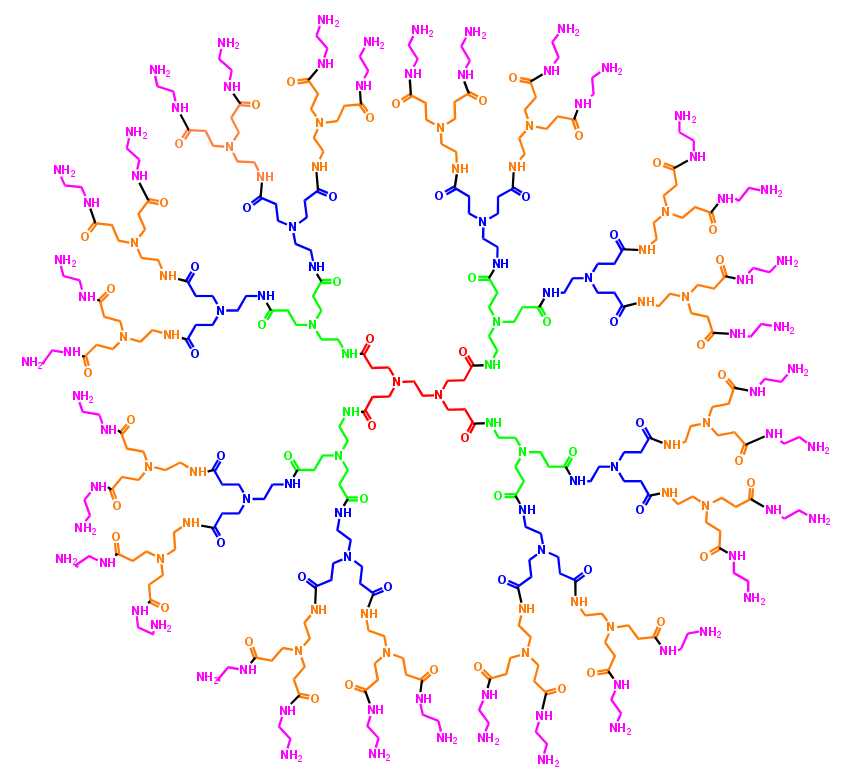
\includegraphics[width=0.45\textwidth]{PAMAM.png}
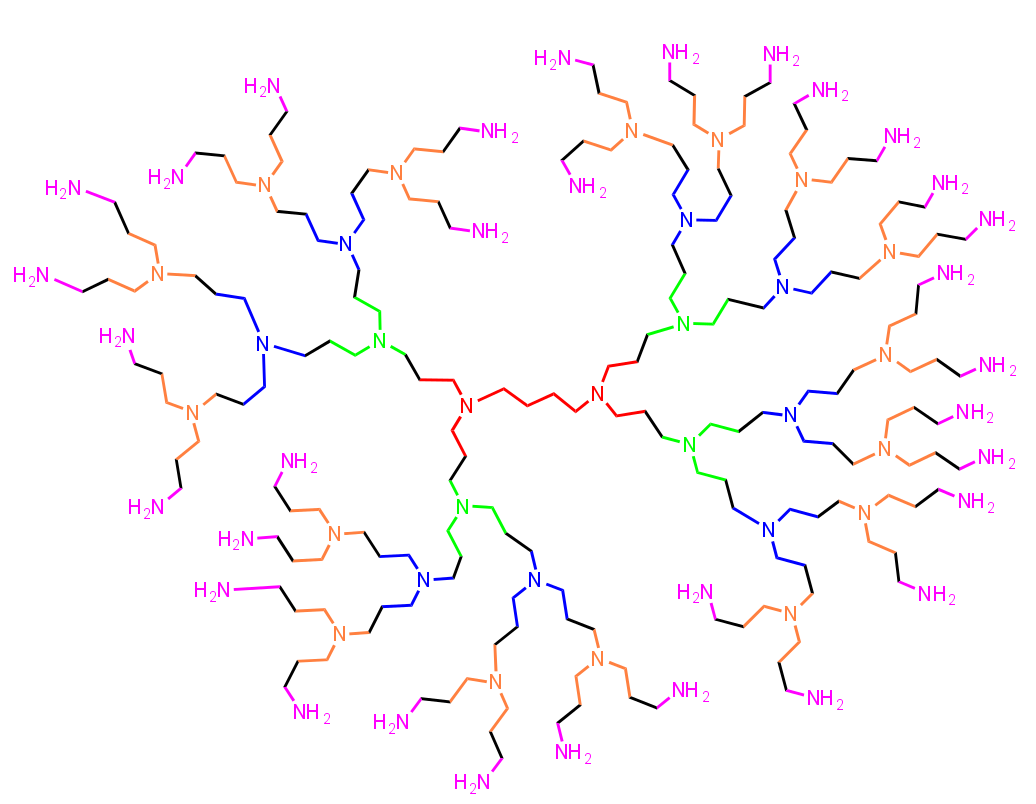
\includegraphics[width=0.45\textwidth]{PPI.png}
\caption{Estrutura química dos dendrímeros Poli(amido amina) (PAMAM) de geração três com núcleo de etileno diamina (EDA) à esquerda e Poli(propileno imina) (PPI) de geração quatro com núcleo de 1,4-diamino butano (DAB) à direita. As cores mostram a camada de blocos intermediários pertencentes à mesma geração. Segundo a nomenclatura utilizada para o PAMAM: O bloco nuclear é mostrado em vermelho, a geração um em verde, a segunda geração em azul, a terceira em laranja e, em rosa, os blocos terminais.}
\label{PAMAMPPI}
\end{figure}

A grande variedade de aplicações atribuídas aos dendrímeros se deve à sua forma tridimensional\cite{Vogtle2000}.
Sua estrutura pode ser dividida em três regiões: a superfície, o espaço entre as cadeias ramificadas e o núcleo do dendrímero\cite{Dykes2001}.
Dependendo da estrutura química da molécula, cada uma dessas regiões pode ter um comportamento distinto e expressar um ambiente químico diferente.
Isso tem verificado às estruturas dendrídicas diversas aplicações em:
Sensores\cite{ChristineValerio1997, Balzani2000},
catalisadores\cite{Kainz2014,Deraedt2017, P.Bhyrappa1996},
processos de separação\cite{Song2017, Song2017a},
\textit{light-harvesting}\cite{Gilat1999, Adronov2000, Andrews2012},
produção de materiais\cite{Gaertner2011, Arshadi2017, Xie2005},
entre outras.
Dentre as aplicações dos dendrímeros, uma de especial interesse é no seu uso como carreadores de fármacos em \textit{Drug-Delivery Systems} (DDS)\cite{Li2010, Svenson2005, Wei2015, Wang2018, Yesil-Celiktas2017}.
Cuja principais regiões utilizadas são as regiões entre as cadeias ramificadas para a solubilização dos fármacos e a superfície para funcionalização e melhorias na seletividade da liberação.
As modificações mais comuns encontradas são a adição de cadeias de Poli(etileno glicol) (PEG) e Poli(óxido de etileno) (PEO) nas cadeias terminais do dendrímero para reduzir sua toxicidade\cite{Sousa2018}.

Como os dendrímeros são altamente personalizáveis, estando sua síntese limitada somente pela criatividade do pesquisador que a está desenvolvendo, muitos novos dendrímeros têm sido relatados na literatura e a definição anterior tem sido estendida recentemente.
De fato, muitas das aplicações podem ser melhoradas com funcionalizações das unidade terminais. 
Nesse âmbito, vêm sido publicados na literatura dendrímeros não-simétricos\cite{Wang2018} (como o Janus\cite{Zhang2014, Gao2014, Dengiz2015}, por exemplo), híbridos\cite{Kavyani2016}, e com funcionalizações na superfície\cite{Barraza2017, Sousa2018, Lee2011, Chooi2010}.

O entendimento da estrutura, das propriedades, do comportamento físico-químico e da interação dos dendrímeros com o meio são informações de vital importância para o conhecimento desse tipo de sistemas, para o desenvolvimento de novas tecnologias e para a projeção de melhorias nas já existentes.
Inicialmente o estudo de dendrímeros foi feito majoritariamente por técnicas experimentais descritas em revisões disponíveis na literatura\cite{Caminade2005, Lizama2016}:
SAXS\cite{Prosa2001, Rathgeber2004, Prosa1997},
SANS\cite{Porcar2008, Ramzi1998, Scherrenberg1998},
RMN\cite{Malveau2003},
UV-Vis\cite{Pande2011},
AFM\cite{Li2000} e
TEM\cite{Jackson1998}.
Contudo, essas técnicas são limitadas e não conseguem dar informação suficiente sobre o comportamento microscópico dos sistemas para que tenhamos um entendimento completo de seu comportamento.

Dadas as limitações de técnicas experimentais, o uso de abordagens teóricas e computacionais é de grande ajuda para o melhor entendimento desses sistemas.
Dentre as diversas técnicas computacionais disponíveis, a dinâmica molecular tem sido amplamente utilizada para o estudo de estruturas dendríticas complexadas com diversas outras moléculas\cite{Bellini2015, Caballero2013, DeFever2015, Jain2013, Kanchi2018, Tanis2009a} e, assim como o foco desse trabalho, simulado somente em solvente para estudar a validade dos campos de força na simulação de dendrímeros\cite{Maingi2012, Maiti2004, Maiti2005, Maiti2008, Opitz2006, Wu2010, Kavyani2014}.

Trabalhos teóricos investigando cadeias lineares de polímeros sugerem que o príncipio da universalidade possa ser usado para cadeias suficientemente grandes.
Isso é, para longas cadeias lineares de polímeros, algumas propriedades do sistema independem de detalhes microscópicos.
Em específico, o tamanho característico $R$ de uma cadeia polimérica em solvente bom aumenta com o grau de polimerização segundo a equação\cite{Ballauff2004}:

\begin{equation}
R=C\alpha N^\nu
\end{equation}
onde $\alpha$ é o comprimento do monômero, $C$ é uma constante não universal e $\nu$ é a constante universal de Flory, em 3 dimensões, $\nu=0.588$ que pode ser calculado por cálculos de grupo de renormalização e simulações.
Esse conceito foi estendido para o estudo de dendrímeros, mas sua validade é questionável já que o grau de polimeziração dos dendrímeros cresce exponencialmente com a geração.
Mas muitos trabalhos computacionais se baseam nessa ideia e buscam uma lei de formação exponencial para uma medida de comprimento característico (principalmente o raio de giro $R_g$, que será discutido na Seção \ref{RaioDeGiro}) utilizando simulação com modelos \textit{bead-spring}\cite{Zhou2006} e por dinâmica browniana\cite{Bosko2011}.
Além disso, Timoshenko \textit{et al}\cite{Timoshenko2002} utilizou Monte-Carlo para estudar a estrutura tridimensional do dendrímero em solventes de diferentes qualidades (solventes bons, no ponto $\theta$ e ruins\cite{Bosko2011}) e chegou à conclusão de que o dendrímero teria uma função de distribuição radial com um máximo na origem quando em solvente bom (vale especificar que, mesmo que formalmente, misturas de dendrímeros sejam uma dispersão devido ao tamanho do dendrímero. A literatura se refere à elas como soluções pois os efeitos disperssantes não são percebidos nas concentrações utilizadas. Por isso, denotaremos por solvente bom um dispersante que interage de forma estabilizante com a estrutura e de solvente ruim o que interagir de forma contrária.).
Esse perfil foi chamado de modelo \textit{dense-core}, sugerindo que a região de maior densidade de átomos do dendrímero encontra-se perto do núcleo.
Porém quando a qualidade do solvente era alterada para um solvente ruim, o perfil de distribuição radial se tornava mais distribuido ao longo do volume da molécula com um platô, ou seja, a densidade radial era quase homogênea ao longo do raio da molécula com um máximo na região terminal.
Esse modelo é chamado de \textit{dense-shell} e o fenômeno de mudança de perfil de densidades com mudanças na qualidade do solvente foi chamado pelos autores de transição \textit{coil-to-globule}.
Como foi mostrado por Balauff \textit{et al}\cite{Ballauff2004} em sua revisão, os trabalhos de simulação por muito tempo divergiram em conclusões sobre o perfil mostrado por Timoshenko \textit{et al}\cite{Timoshenko2002}.
Entretanto, hoje é aceito que, em água, o PAMAM e o PPI são melhores descritos pelo modelo de \textit{dense-core} devido à alta taxa de \textit{back-folding} dos seus blocos terminais.
\textit{Back-folding} é a interação dos monômeros terminais do dendrímero com seus blocos intermediários, fazendo com que as ramificações se virem para o interior de sua estrutura ao invés de se apresentar como uma estrutura completamente aberta (esse fenômeno será melhor descrito nas Seções \ref{PAMAMEstrutura} e \ref{PPIEstrutura}). 
O estudo computacional de dendrímeros em solventes explícitos que não sejam bons ainda não está bem desenvolvido, mas simulações no vácuo sugerem que o modelo mostrado por Timoshenko \textit{et al}\cite{Timoshenko2002} é robusto.
Contudo, é possível ver algum indício de transição \textit{coil-to-globule} em bons solventes dependendo da estrutura do dendrímero.
Simulações de PAMAM funcionalizado com PEG\cite{Lee2011} dão indícios de que um grande grupo terminal pode impedir o processo de \textit{back-folding} e dar origem à um modelo mais parecido com um \textit{dense-shell}.

Trabalhos de simulação têm sido mais amplamente empregados para o estudo desses sistemas desde o trabalho de Tomalia \textit{et al}\cite{Tomalia1990} em 1990 onde o PAMAM foi simulado utilizando o campo de força AMBER\cite{Weiner1984} por alguns poucos picossegundos.
Nesse estudo, eles não obtiveram bons valores no cálculo do diâmetro da molécula em relação aos dados experimentais disponíveis na época, um erro que aumenta com a geração do dendrímero.
Mas esse foi um artigo importante pois, além de mostrar a viabilidade da simulação de dendrímeros, os autores dão inicio ao estudo dessa classe de moléculas falando sobre sua versatilidade, potenciais aplicações e descrevendo sua estrutura.

Focando no PAMAM, após esse estudo de Tomalia \textit{et al}\cite{Tomalia1990}, Lee \textit{et al}\cite{Lee2002} fizeram simulações em diferentes condições de pH considerando gerações de $2$ à $6$ em solvente implícito utilizando o campo de força Consistent Valence Force Field\cite{Lifson1979} (CVFF).
Nesse estudo, uma mudança de um regime \textit{dense-core} em pH básico para algo próximo ao \textit{dense-shell} em pH ácido foi observada.
Porém, em pHs mais baixos não há a ocorrência de \textit{back-folding}, contrariando os estudos teóricos anteriores.
Essa questão pode ser atribuída à consideração de um solvente implícito. 
Mostrando que efeitos entrópicos são de grande importância na descrição da estrutura dos dendrímeros.

Em 2004, Maiti \textit{et al}\cite{Maiti2004} estudaram o PAMAM de gerações $1$ à $11$ em vácuo considerando a protonação em pH alto, ou seja, o dendrímero desprotonado utilizando o campo de força Dreiding\cite{Mayo1990}.
Segundo os autores, a condição de vácuo é uma boa aproximação para supor um solvente ruim.
O raio de giro calculado foi comparado com dados de SAXS e SANS e, para todas as gerações, os valores obtidos subestimaram os dados experimentais, em média, por $0.4$ nm.
Quanto à estrutura, esse estudo obteve a distribuição radial esperada para o sistema em solvente ruim.
Existe um platô nas curvas de densidade radial indicando uma maior tendência ao modelo \textit{dense-shell}.
Reforçando a interpretação dos resultados em solvente ruim, essas simulações foram capazes de reproduzir a predição teórica de Sheng \textit{et al}\cite{Sheng2002} de que, em solvente ruim, o $R_g \sim N^{1/3}$ (onde $R_g$ é o raio de giro e $N$ é o número de monômeros).
Ainda em 2004, Lin \textit{et al}\cite{Lin2005} realizaram um estudo sobre a dinâmica de moléculas de água em regiões bem definidas do PAMAM.
O espaço próximo à superfície do dendrímero foi separado em domínios \textit{bulk} (longe da superfície), superficial (bem próximo ao limite entre dendrímero e solvente livre), e enclausurado (na região interna da molécula) (para maiores detalhes, ver Figura 2 no estudo original).
Foi relatado que em todas as regiões definidas, as moléculas de água têm um comportamento difusional bem distinto da água livre.
De fato, moléculas de água próximas à superfície do dendrímero tem seu coeficiente de difusão significativamente reduzido mostrando que mesmo à $1.2$ nm da superfície dendrítica, as moléculas de água ainda são fortemente influenciadas pela presença do dendrímero.
Esse padrão de comportamento pode ser importante nas considerações feitas nos modelos utilizados para o cálculo do raio de giro através das técnicas de SANS e SAXS, como será discutido mais a frente.

Em 2005, Maiti \textit{et al}\cite{Maiti2005} realizaram um estudo avaliando a influência do pH considerando solvente explícito para as gerações de 4 à 6. 
Em relação ao estudo de 2004, eles mostraram que a consideração explícita do solvente melhorou a adequação dos cálculos em relação aos experimentos.
Também, a consideração de moléculas explícitas causou o aparecimento de um pico muito bem definido na curva de densidade radial na região próxima ao centro do dendrímero em algumas gerações.
Em acordo com os resultados teóricos e obtidos por outras técnicas de simulação: quando em um solvente bom (como é o caso da água) a descrição correta é dada pelo modelo \textit{dense-core}.
Mas para algumas gerações essa interpretação ainda foi difícil de ser feita.

Opitz \textit{et al}\cite{Opitz2006}, realizaram simulações de dinâmica molecular utilizando água como solvente implícito e também compararam o uso de metanol como solvente explícito e implícito utilizando o campo de força General Amber Force Field (GAFF)\cite{Wang2004}.
O metanol, assim como a água, é um solvente bom.
Porém, o menor número de possibilidades de se formar interações do tipo ligação de hidrogênio faz com que ele seja um solvente pior que a água.
Em geral, os raios de giro calculados para os dendrímeros solvatados em metanol são maiores que em água, indicando que eles interagem mais fracamente com as moléculas de solvente em suas cavidades possibilitando sua expansão.
O estudo das estruturas obtidas ao considerar, ou não, o solvente explícito mostra o resultado esperado: existe uma menor ocorrência de \textit{back-folding} quando considerado uma abordagem com solvente implícito.
Isso reforça a ideia de que consideração explícita do solvente é de extrema importância para a conformação correta da estrutura dendrítica.

Maiti e Messina\cite{Maiti2008} estudaram a distribuição do contraíon na solução para as gerações de $3$ à $7$ em pH neutro com solvente explícito e utilizando o campo de força Dreiding\cite{Mayo1990}.
Embora ainda haja um certo desacordo em relação ao raio de giro quando comparado com resultados experimentais de SAXS e SANS (da ordem de $\sim 0.5$ nm), as funções de distribuição radial calculadas estão de acordo com a predição teórica do modelo \textit{dense-core}.
Eles também calcularam a função de distribuição radial para analisar a distribuição de contra-íons ao redor do dendrímero.
A distribuição de íons cloreto se concentrou no interior e na região superficial, onde há a maior concentração de carga.
A grande concentração no interior do dendrímero, se deve ao fato de blocos terminais que realizam \textit{back-folding} atraírem contra-íons para o interior da estrutura.

Em 2009, Tanis e Karatasos publicaram dois artigos com forte motivação em DDS.
No primeiro deles\cite{Tanis2009a} foi estudado a associação do ibuprofeno (um anti-inflamatório) com o PAMAM de geração 3 verificando efeitos do pH na complexação.
Nesse estudo, foi utilizado o campo de força AMBER\cite{Weiner1984} e solvatação explícita com moléculas de água TIP3P.
Eles relataram, através do monitoramento da distância média entre o centro de massa das moléculas de ibuprofeno e do dendrímero, que em pH alto e neutro o complexo se manteve estável durante toda a dinâmica.
Enquanto em pH baixo, rapidamente o ibuprofeno é expulso das cavidades do dendrímero e a distância entre seus centros de massa aumenta ao longo da simulação.
Segundo os autores, isso se deve ao fato da estrutura se apresentar com uma forma mais aberta quando em pH ácido.
Em seu segundo trabalho\cite{Tanis2009}, eles estudaram o comportamento do PAMAM de gerações 3 e 4 quando complexado com poli(óxido de etileno) (PEO) com mesmo número de monômeros que o número de aminas primárias (blocos terminais) no dendrímero.
Por análise do número de ligações de hidrogênio formadas entre o dendrímero e o PEO nos diferentes pHs, foi relatado que há a interação mais forte entre eles quanto menor for o pH.

Bellini \textit{et al}\cite{Bellini2015} estudaram a associação da rifampicina com o PAMAM de geração $4$ utilizando solvente explícito e o campo de força OPLS-AA\cite{Jorgensen1996}.
Eles mostram, por meio das funções de distribuição radial, que a associação com a rifampicina causa uma mudança perceptível na estrutura interna do dendrímero.
E pela análise da distância entre os centros de massa de cada uma das moléculas de rifampicina e do PAMAM, pode-se ver que em pH neutro, o complexo é estável ao longo de toda a dinâmica.
Mas em pH baixo, essa distância rapidamente aumenta e podemos ver que em torno de $40$ ns a maioria das moléculas de rifampicina associadas foram expulsas da região interna do dendrímero.

Nos últimos anos, poucos estudos experimentais foram dedicados à investigar a dependência do raio de giro com o pH do meio\cite{Porcar2008, Nisato2000}. O único estudo sistemático fez uso da técnica SANS e considerou as gerações de 3 à 6 do PAMAM em três valores distintos de pH. 
Um segundo estudo de SANS considerou apenas a geração 8.
Esses sugerem que o raio de giro seria invariante em relação à mudanças no pH.
Porém, praticamente nenhum trabalho teórico ou computacional conseguiu reproduzir esse comportamento.
Maiti e Goddard III\cite{Maiti2006} simularam o PAMAM de geração $8$ para comparar com o trabalho de Nitaso \textit{et al}\cite{Nisato2000} e mostram que o inchaço encontrado nas simulações é condizente com o comportamento energético do sistema.
Os autores então sugerem que o uso de modelos para o cálculo do raio de giro a partir da curva de intensidade de espalhamento pode estar introduzindo algum erro nos resultados experimentais.
Liu \textit{et al}\cite{Liu2009} conseguiram reproduzir esse fenômeno de variação do pH sem o inchaçodo dendrímero, mas para isso um novo termo precisou ser parametrizado e adicionado ao campo de força.
Eles atribuíram esse termo à consideração explícita das interações de hidrogênio intramoleculares.
Em 2012, Wu \textit{et al}\cite{Wu2012} utilizou os resultados obtidos por Lin \textit{et al}\cite{Lin2005} de que a mobilidade da água é fortemente afetada próximo à superfície do dendrímero.
Sob a justificativa de que o resultado de SANS seria sensível à mudanças de densidade local no sistema, eles calcularam a curva de fator de estrutura intra-dendrímero de três formas diferentes:
($i$)  utilizando somente as moléculas do PAMAM propriamente dito,
($ii$) utilizando, além do PAMAM, moléculas de água interfacial (até $0.4$ nm dos átomos do dendrímero),
($iii$) considerando uma esfera virtual que continha o PAMAM e todas as moléculas de água e contra-íons dentro dela.
Com essa abordagem, a consideração da esfera virtual faz com que haja um acordo melhor com fator de estrutura experimental do que quando não considerada.
Mas para altos valores do vetor de onda $Q$, ainda há um erro considerável.
Considerando os trabalhos experimentais que utilizam a técnica SAXS, o trabalho de Dootz \textit{et al}\cite{Dootz2011} mostra um inchaço do PAMAM com o abaixamento do pH, como relatado pela maioria dos trabalhos teóricos e computacionais até a presente data.
Contudo, o grau de protonação utilizado nesse trabalho dificulta a comparação do valor absoluto do diâmetro do PAMAM relatado.
Como eles efetuam os experimentos em pHs onde o dendrímero não está totalmente protonado nem totalmente desprotonado como nos meios ácido e básico sugeridos comumente em trabalhos computacionais, o único resultado que pode ser comparado quantitativamente é o resultado em meio neutro.
Esse apresenta um excelente acordo com os resultados da presente dissertação.
De forma qualitativa, as conclusões do trabalho de Dootz \textit{et al}\cite{Dootz2011} estão em bom acordo com os trabalhos teóricos.

Recentemente, Kim \textit{et al}\cite{Kim2014} e Kanchi \textit{et al}\cite{Kanchi2018} calcularam a energia livre de adsorção do PAMAM em membranas lipídicas.
Nesses estudos, somente o campo de força GROMOS conseguiu predizer o valor negativo da variação de energia livre, em acordo com resultados experimentais.
Nesses estudos, eles utilizaram o campo de força GROMOS86, uma versão muito antiga do conjunto de parâmetros.

Considerando as simulações do PPI,
em 1998, Scherrenberg \textit{et al}\cite{Scherrenberg1998} efetuaram experimentos de SANS e cálculos de dinâmica molecular utilizando o CVFF\cite{Lifson1979} como campo de força para dendrímeros de geração $1$ à $5$ com dois blocos terminais distintos (grupo NH$_2$ e $CN$).
Os raios de giro calculados subestimaram os resultados de SANS em todas as gerações maiores que $1$ para o PPI terminado em NH$_2$ e a função de distribuição radial obtida é mais homogeneamente distribuida, diferentemente dos modelos observados para o PAMAM e por estudos teóricos.
Brocorens \textit{et al}\cite{Brocorens2005} simularam o PPI de gerações $1$ a $7$ no vácuo com três blocos terminais distintos utilizando o Dreiding\cite{Mayo1990} como campo de força.
Eles relataram que com o aumento da geração, a densidade próximo do núcleo do dendrímero aumenta devido à interações de hidrogênio intramoleculares, mas o grau de \textit{back-folding} não segue esse aumento.
Wu\cite{Wu2010} utilizou um campo de força híbrido misturando parâmetros do COMPASS\cite{Sun1998} com do OPLS-AA\cite{Jorgensen1996} de forma arbitrária, prática que não garante o funcionamento do campo de força à priori, para simular o PPI de geração $5$ em solvente explícito.
Como será melhor discutido na Seção \ref{PPITamanho} o perfil de protonação do PPI não é bem definido e resultados de titulação mostram resultados distintos dos observados para o PAMAM.
Nesse estudo, Wu \textit{et al} considerou que em pH ácido e básico o PPI está totalmente protonado e desprotonado, respectivamente.
Já em pH neutro, as aminas primárias (terminais) e todas as camadas ímpares estarão protonadas.
Os resultados obtidos superestimam um pouco os dados experimentais de SANS e, curiosamente, não há mudança perceptível entre as simulações em pH neutro e baixo.
As funções de distribuição radial calculadas indicam que há uma hidratação da estrutura interna do dendrímero quando em pH neutro e baixo, provavelmente devido sua maior carga e estrutura mais aberta.
Elas também mostram um alto grau de \textit{back-folding} e o perfil de densidade muda de uma distribuição mais homogênea para uma mais parecida com o modelo \textit{dense-shell} quando passamos do pH alto para o neutro e baixo.

Jain \textit{et al}\cite{Jain2013} simularam PPI de geração 5 com núcleo de EDA em solvente explícito utilizando o campo de força GAFF\cite{Wang2004}.
Eles estudaram a associação de 3 fármacos com o dendrímero em diferentes pHs com um perfil de protonação similar ao utilizado por Wu \textit{et al}\cite{Wu2010}.
A validação do raio de giro foi feita principalmente por comparação com outros trabalhos de simulação onde o PPI foi simulado com o núcleo de DAB.
Mas mesmo com essa diferença, os resultados estão em excelente acordo.
O estudo com os fármacos chegou à conclusão que com o dendrímero completamente protonado, a expulsão de moléculas de seu interior é mais facilitada. 
Contudo, dependendo do fármaco, a associação é estável, ou instável, independentemente do pH.

DeFever e Sarupria\cite{DeFever2015} utilizaram o campo de força OPLS-AA\cite{Jorgensen1996} para simular o PPI de gerações $3$ à $6$ complexado com naftaleno em solvente explícito.
Eles simularam somente o sistema em pH neutro e consideraram que somente as aminas terminais estariam protonadas nesse pH, em desacordo com trabalhos anteriores disponíveis na literatura.
Nesse estudo, eles mostraram que o naftaleno interage majoritariamente com a superfície do PPI e fica alocado nas cavidades mais superficiais do dendrímero.

Até a presente data, os campos de força mais utilizados foram Amber\cite{Weiner1984}, GAFF\cite{Wang2004}, CVFF\cite{Lifson1979}, Dreiding\cite{Mayo1990}, OPLS-AA\cite{Jorgensen1996}, COMPASS\cite{Sun1998} e modelos \textit{Coarse-grained}\cite{Smeijers2016, Freire2015, Maiti2009, Wang2012}.
São poucas as referências com campos de força GROMOS.
O campo de força GROMOS é notável devido sua estratégia de parametrização focada na reprodução de propriedades termodinâmicas, e não estruturais.
Isso pode conferir um maior poder preditivo em processos de interesse bioquímico como a partição de componentes em meios de diferente polaridade, complexação e agregação, enovelamento e ligação entre proteína e ligante.
Com base na filosofia de parametrização do GROMOS, o campo de força GROMOS 53A6$_{\text{OXY}}$\cite{Horta2011} foi desenvolvido em 2011 com o objetivo de unificar dois de seus antecessores: o 53A5\cite{Oostenbrink2004}, desenvolvido para líquidos puros, e o 53A6\cite{Oostenbrink2004}, para simulações biomoleculares.
O 53A6$_{\text{OXY}}$ foi aprimorado e deu origem ao atual \textit{GROMOS-compatible} 2016H66\cite{Horta2016}, utilizado na presente dissertação.
As principais vantagens do uso desse campo de força são: 
($i$)   Como seu conjunto de parametrizaçao foi composto por diversas moléculas orgânicas constintuintes de blocos de construção de muitos dendrímeros (como aminas, amidas e esteres), é intuitivo acreditar que ele se adequará bem à simulação dessa classe de moléculas;
($ii$)  O interesse em se estudar alternativas para DDS justificam a escolha de um campo de força validado para simulação dos fármacos que serão complexados com os dendrímeros no futuro e, também, possa ser utilizado para simular as funcionalizações comumente colocadas na superfície;
($iii$) Seu modelo \textit{united-atoms}, que trata hidrogênio não polares de forma implícita, simplifica grupo CH$_n$ e o trata como um único pseudo-átomo. Isso torna a simulação menos custosa computacionalmente sem grade perda de acurácia nos resultados;
($iv$)  Compatibilidade com o software PyPolyBuilder que facilita o preparo das topologias e coordenadas iniciais (descrito na Seção \ref{PyPolyBuilder}).


\chapter{Objetivo Geral}
Esse trabalho tem como objetivo geral validar o uso do campo de força 2016H66\cite{Horta2016} para a simulação de dendrímeros por meio de comparação com trabalhos experimentais e de simulação disponíveis na literatura. 

Para isso, o raio de giro ($R_g$) será calculado e comparado com resultados de experimentos de espalhamento de neutrons e de raio-X a baixos ângulos (SANS e SAXS, respectivamente) e de simulações.

Também, razões de aspecto, asfericidade e perfis de distribuição radial serão calculadas e comparadas com trabalhos computacionais, já que técnicas experimentais não conseguem obter informações quantitativas sobre essas propriedades.

\pagebreak



\chapter{Embasamento teórico}
No que diz respeito à modelagem molecular, diversas técnicas computacionais podem ser empregadas para o estudo de sistemas microscópicos.
Alguns desses métodos se baseiam na teoria da mecânica quântica para descrever satisfatoriamente o comportamento eletrônico do sistema. 
Uma vez que elétrons são partículas intrinsicamente quânticas, sua descrição correta só é possível com esses métodos.
Como sistemas químicos são governados por processos eletrônicos, técnicas de simulação que levem em conta essa característica quantizada do sistema devem ser utilizados.
Porém, cálculos quânticos são de elevado custo computacional e mesmo com os grandes avanços em eficiência de algoritmos e novos métodos para reduzir esse custo, o estudo de grandes sistemas ainda é um problema nos dias de hoje.

Muitas vezes estamos interessados somente em propriedades físicas (não-eletrônicas) do sistema. Nesses casos, podemos fazer algumas aproximações com o objetivo de simplificar o tratamento teórico.
Uma primeira consideração que pode ser feita é considerar que os átomos como um todo sejam esferas modeladas por um potencial efetivo incluindo de forma média e implícita as propriedades eletrônicas, o que permite a eliminar o cálculo explícito relativo aos graus de liberdade dos elétrons..
A função de energia potencial que descreve o sistema deve ser parametrizada com o auxílio de propriedades experimentais ou de cálculos quânticos de alto nível.
O conjunto de parâmetros e de formas funcionais utilizados para a construção do potencial é chamado de campo de força.
Após parametrizado, o campo de força pode ser utilizado por alguma das técnicas de simulação clássica. Dentre essas técnicas, destacamos a dinâmica molecular clássica\cite{Jensen2017}.

\section{Dinâmica Molecular}

Dinâmica molecular consiste em resolver as equações de movimento da mecânica clássica para um sistema de muitos corpos.
Do ponto de vista do esforço computacional, a dinâmica molecular clássica (onde o hamiltoniano considerado é clássico) é uma técnica sigficativamente menos custosa que os métodos quânticos e, por isso, torna possível o estudo de sistemas maiores.

%ela é uma técnica sigficativamente mais leve que os métodos quânticos e, por isso, se torna possível o estudo de sistemas maiores.

Nesta técnica, é necessário a definição das posições e velocidades iniciais dos átomos constintuintes do sistema.
Com base no campo de força e nas posições atuais, podemos calcular a força atuante em cada um dos átomos do sistema.
Então resolve-se a equação de Newton para calcular sua nova posição em um passo futuro.
O novo conjunto de coordenadas é então utilizado para recalcular as forças e assim pode-se avaliar a evolução temporal do sistema com base na integração numérica das equações de movimento\cite{Frenkel2002}.

Uma vez obtida a trajetória do sistema, pode-se fazer uso da mecânica estatística para calcular as propriedades desejadas do sistema. 

\subsection{O campo de força}

Pode-se descrever a forma funcional do campo de força de diversas formas.
Uma possibilidade, a que foi utilizada neste trabalho, é\cite{Leach2001}:

\begin{equation}
\begin{aligned}
V(r) = &\sum_{b} \frac{k_{b}}{2}(r_{b,eq}-r_{b})^2 \;+\\
       &\sum_{a} \frac{k_{a}}{2}(\theta_{a,eq}-\theta_{a})^2\;+\\
       &\sum_{d} \frac{V_t}{2}(1+cos(n\omega_{d}+\gamma))\;+\\
       &\sum_{i} \frac{V_i}{2}(\xi_{i,eq} - \xi_i)^2\;+\\
       &\sum_{i=1}^N \sum_{j=i+1}^N \left(4\epsilon_{ij}\left[\left(\frac{\sigma_{ij}}{r_{ij}}\right)^{12} - \left(\frac{\sigma_{ij}}{r_{ij}}\right)^{6}\right] + \frac{q_i q_j}{4\pi \epsilon_0 r_{ij}} \right)
\end{aligned}
\label{FF}
\end{equation}

onde $k_{b}$, $r_{b,eq}$, $k_{a}$, $\theta_{a,eq}$, $V_t$, $n$, $\gamma$ e $\xi_{i,eq}$ são parâmetros dos potenciais ligados; $\epsilon_{ij}$, $\sigma_{ij}$, $q_i$, $q_j$ são parâmetros dos potenciais não ligados e devem ser ajustados empiricamente.
A variáveis $r_{b}$, $r_{ij}$, $\theta_{a}$, $\omega_{d}$ e $\xi_{i}$ são a distância entre dois átomos ligados e não ligados, o ângulo formado por três átomos ligados em série, o ângulo formado pelo torsional de diedro próprio e o impróprio, respectivamente.
Os termos da Equação \ref{FF} são referentes aos graus de liberdade ilustrados na Figura \ref{CampoDeForca}.

\begin{figure}[ht!]
\centering
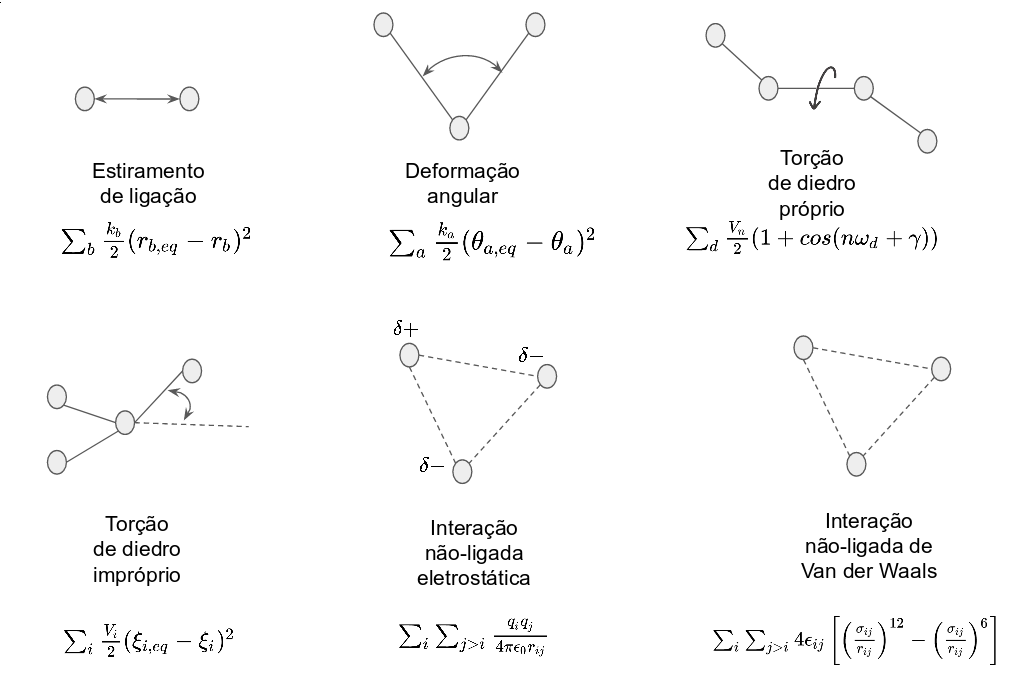
\includegraphics[width=0.9\textwidth]{CampoDeForca.png}
\caption{Representação esquemática das deformações responsáveis pela energia potencial no sistema. Pela ordem de aparecimento dos termos na Equação \ref{FF}, estiramento de ligação, estiramento angular, estiramento de diedro e interações não-ligadas.}
\label{CampoDeForca}
\end{figure}

A forma como os átomos são tratados no campo de força também pode ser diferente entre cada modelo.
A forma mais completa é conhecida como uma abordagem \textit{all-atoms} e consiste em incluir, explicitamente, todos os átomos do sistema nos seus cálculos.
A fim de possibilitar a simulação de sistemas ainda maiores, alguns átomos podem ser tratados em conjunto como um pseudo-átomo.
Essa abordagem é conhecida como \textit{united-atoms} ou \textit{coarse grained}, dependendo de quantos átomos são omitidos do seu modelo\cite{Allen2017}.
Como discutido anteriormente, o 2016H66\cite{Horta2016} é um modelo \textit{united-atoms}, ou seja, seus átomos de hidrogênio apolares são tratados em conjunto com os átomos de carbonos aos quais estão ligados.
Dessa forma, os grupos CH$_n$ são tratados como um único pseudo-átomo.

A definição da forma funcional, o valor dos parâmetros propriamente ditos, assim como outros parâmetros utilizados na simulação (como o raio de corte $r_c$ do modelo, por exemplo, que veremos mais a frente) compõem o campo de força.
É importante ressaltar que o conjunto de condições utilizadas na parametrização é de significativa importância para a reprodutibilidade dos resultados obtidos com os campos de força disponíveis na literatura.
Como mostrado em um estudo sistemático por Gonçalvez \textit{et al}\cite{Goncalvez2018}, uma mudança arbitrária das condições de simulação podem causar mudanças substanciais nos resultados obtidos.

\subsection{Integração das equações de movimento}

A princípio, as funções que regem as equações de movimento são contínuas. Para que possamos integrá-las numéricamente precisamos discretizar o tempo e utilizar um algoritmo de integração.
Dentre os algoritmos conhecidos, alguns poucos se tornaram populares para uso em dinâmica molecular por atenderem os requisitos de conservação de energia, reversibilidade temporal e por serem bem escaláveis quanto ao custo computacional\cite{Frenkel2002}.
O algoritmo utilizado nesse trabalho foi o \textit{leap-frog}, que usa as seguintes relações para a evolução temporal da posição e da velocidade\cite{Leach2001}:

\begin{equation}
\begin{aligned}
& \textbf{r}(t+\delta t)=\textbf{r}(t)+\delta t \times \textbf{v}(t+\frac{1}{2}\delta t)\\
& \textbf{v}(t+\frac{1}{2}\delta t)=\textbf{v}(t-\frac{1}{2}\delta t)+\delta t \frac{\textbf{F}(t)}{m}
\end{aligned}
\label{leap-frog}
\end{equation}
onde $\textbf{r}$ e $\textbf{v}$ são os vetores de coordenadas e velocidade, respectivamente, $\delta t$ é o incremento no tempo (ou passo de tempo), $\textbf{F}$ é a força resultante na partícula e $m$ a sua massa.

O \textit{leap-frog} tem a vantagem, em relação ao algoritmo de Verlet (um dos mais utilizados em simulações de dinâmica molecular), de incluir a velocidade explicitamente no seu equacionamento, dessa forma a velocidade é mais consistentemente calculada.
Uma desvantagem, é que o conjunto de coordenadas e de velocidades não são avaliados no mesmo instante de tempo. 
Como pode ser visto nas relações mostradas na Equação \ref{leap-frog}, a integração é feita primeiro na velocidade, calculando o seu valor em um tempo de $\frac{1}{2}\delta t$ futuro. E então esse valor de velocidade é utilizado para calcular as coordenadas em $\delta t$.
Portanto, estimativas sobre o valor total de energia (soma da cinética e potencial) não podem ser avaliadas diretamente com o uso desse algoritmo.
Contudo, ele já foi altamente validado em trabalhos da área e, como as propriedades de interesse (Ver \ref{Propriedades}) dependem unicamente das posições, essa desvantagem não será um problema para este estudo\cite{Leach2001}.

A simples integração das equações de movimento não possibilita o controle das condições de simulação (principalmente temperatura e pressão).
De fato, é possível mostrar que uma simulação desse tipo mantém o número de partículas, o volume do sistema e a energia contantes.
Ou seja, o conjunto estatístico, ou o \textit{ensemble}, natural é o micro-canônico\cite{Tuckerman2010}.
Como os experimentos são, geralmente, realizados à temperatura e pressão constantes, as equações de movimento são, geralmente, modificadas para fornecer o ensemble isotérmico-isobárico.
Isso é feito adicionando termos extras no hamiltoniano que levem em conta um banho externo para controle da pressão e da temperatura.

\subsection{Outros ensembles}

Da mecanica estatística, sabe-se que o valor médio da energia no ensemble canônico é proporcional à termeratura\cite{Leach2001}.
De fato:

\begin{equation}
{\left< {H} \right>}_{NVT} = \frac{3}{2}Nk_bT ,
\end{equation}
onde $H$ é o Hamiltoniano, $N$ é o número de partículas, $k_b$ a constante universal de Boltzmann e $T$ a temperatura.

Na ausência de campo externo, o Hamiltoniano de um gás ideal é dado pela soma as energias cinéticas de todas as partículas do sistema.
De forma que podemos isolar a temperatura da seguinte forma:

\begin{equation}
T=\frac{1}{2} \sum_{i=1}^{N} {\frac{2}{3}\frac{m_i v_i^2}{Nk_b}}
\end{equation}
onde $m_i$ e $v_i$ são,respectivamente, a massa e a velocidade da partícula $i$ no somatório.

A primeira forma utilizada para controle da temperatura foi idealizada por Woodcock\cite{Woodcock1971} em 1971 e consiste em multiplicar as novas velocidades por um fator de escala para forçar o sistema a manter a mesma temperatura.
Isto é, ele propôs que a variação de temperatura fosse escrita da seguinte forma:

\begin{equation}
\Delta T = T_{new} - T_{curr}=\frac{1}{2} \sum_{i=1}^{N} {\frac{2}{3}\frac{m_i (\lambda v_i)^2}{Nk_b}} - \frac{1}{2} \sum_{i=1}^{N} {\frac{2}{3}\frac{m_i v_i^2}{Nk_b}}
\end{equation}
onde $T_{new}$ é a temperatura no passo de integração seguinte, $T_{curr}$ a temperatura no atual passo e $\lambda$ é o fator de escala.

Que pode ser reescrito como:

\begin{equation}
\begin{aligned}
&\Delta T = (\lambda ^2 - 1) T_{curr}\\
&\text{com} \; \lambda =  \sqrt{\frac{T_{new}}{T_{curr}}}
\end{aligned}
\end{equation}

Dessa forma, ao selecionar $T_{new}$ fazemos com que o sistema corrija as velocidades de forma a manter $T_{curr}$ em torno de um valor próximo de $T_{new}$.

Outra forma mais utilizada hoje em dia é controlar a temperatura com base no acoplamento com um banho externo mantido à temperatura constante.
Esse método é uma generalização do metódo de Woodcock\cite{Woodcock1971}.
Ele foi desenvolvido por Berendsen\cite{Berendsen1984} em 1984 e é largamente utilizado até hoje.
Nele, associamos a variação da temperatura com a diferença entre o banho externo e o sistema:

\begin{equation}
\frac{dT(t)}{dt} = \frac{1}{\tau}\left( T_{bath}-T(t) \right)
\end{equation}
onde $\tau$ é uma constante de acoplamento que determina o quão fortemente acoplado os sistemas estão, $T_{bath}$ é a temperatura do banho externo e $T(t)$ é a temperatura no sistema simulado.

Esse método dá uma variação exponencial na temperatura do sistema até a convergência para a temperatura do banho.
A cada passo, a temperatura é atualizada de:

\begin{equation}
\Delta T = \frac{\delta t}{\tau}\left( T_{bath}-T(t) \right)
\end{equation}

Essa variação fornece um fator de escala $\lambda$ com a forma:

\begin{equation}
\lambda ^2 = 1 + \frac{\delta t}{\tau}\left( \frac{T_{bath}}{T(t)} - 1 \right)
\end{equation}

Dependendo do valor de $\tau$, o acoplamento pode ser fraco e demorar muito para estabilizar a temperatura do sistema, ou forte e inserir ruidos na variação da temperatura.

Uma abordagem semelhante pode ser feita para a pressão, supondo um ``reservatório de volume'' externo que troca volume com o sistema a fim de mantê-lo ao redor de uma pressão definida.
Seguindo o formalismo de Berendsen mostrado anteriormente, é possível chegar em expressões análogas para a pressão que são conhecidos como o barostato de Berendsen, assim como as equações para a temperatura são conhecidas como o termostato de Berendsen.
Extensões, melhorias e outros modelos de acoplamento foram propostos na literatura e são igualmente utilizados atualmente.
Mas como a ideia base da maioria das abordagens é a exibida aqui, não descreveremos cada um dos modelos existentes\cite{Leach2001}.

\subsection{Avaliação da Força}

Sistemas macroscópicos, em geral, possuem um número enorme de moléculas (da ordem de um mol de moléculas).
Isto é, para simular um sistema com apenas um sexto de mol de qualquer substância, seria necessário computar a força entre, aproximadamente, $10^{23}$ moléculas.
Mesmo que o tempo gasto por um computador para efetuar as contas seja muito rápido, a grande quantidade de átomos inviabiliza o cálculo de um sistema dessa escala de tamanho.
Por outro lado, caso o sistema fosse reduzido à uma caixa com alguns poucos átomos, os efeitos do confinamento da substância acarretaria erros nos cálculos das propriedades do sistema de macroscópico de interesse.
Para conseguir simular um sistema de larga escala sem os efeitos de parede causada pela introdução artificial de uma caixa de simulação, é adotada a condição de contorno periódica.
O que é feito, como ilustrado na Figura \ref{RC}, é considerar cópias do sistema simulado em todas as direções.
Dessa forma, somente o sistema central é simulado e as as cópias têm o mesmo comportamento.
De fato, existe a introdução de uma periodicidade inexistente em sistemas reais, mas isso pode ser contornado considerando uma caixa grande o suficiente para que a influência dessa periodicidade artificial possa ser desprezada.

É necessário calcular a força atuante em cada átomo para resolver a equação de movimento para eles.
Pelo princípio da superposição, força em cada um dos átomos é avaliada como uma soma da contribuição de cada interação atuante no mesmo.
Como o campo de força é escrito em termos da energia potencial, as forças podem ser obtidas por: 

\begin{equation}
F=-\nabla V
\end{equation}

Formalmente, os somatórios correm sobre todos os átomos presentes na simulação.
Mas como visto anteriormente, a representação periódica leva a um sistema com infinitos átomos.
Logo, seria impossível avaliar os somatórios sobre todos os átomos.
Contudo, átomos mais distantes praticamente não contribuem dada sua fraca interação devido sua grande distância em relação ao átomo de referência.
É sabido que a avaliação da força é uma das etapas mais lentas nos cálculos de dinâmica molecular, em especial dos termos não-ligados, por isso é evitado calcular a interação entre átomos muito distantes por ela ser praticamente nula.
A fim de agilizar essa etapa, comumente é utilizado um raio de corte $r_c$ como uma distância máxima em que as interações são consideradas\cite{Frenkel2002}, como ilustrado na Figura \ref{RC}.

\begin{figure}[ht!]
\centering
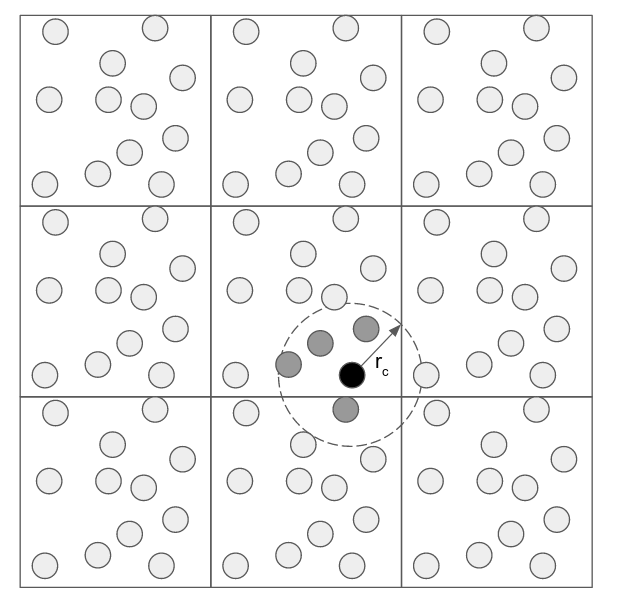
\includegraphics[width=0.5\textwidth]{rc.png}
\caption{Ilustração das condições de contorno periódicas e a consideração de um raio de corte. 
O átomo em preto é o átomo sobre o qual a força está sendo calculada.
O raio de corte é ilustrado por meio do círculo pontilhado.
Os átomos em cinza, dentro do círculho, são os considerados para o cálculo da força no átomo central.}
\label{RC}
\end{figure}

Devido à forma funcional dos potenciais, conforme indicado pela Figura \ref{LJCOUL}, o potencial de Lennard-Jones converge mais rapidamente para zero do que o de Coulomb.
Dessa forma, pode-se definir um raio de corte que contenha todas as interações não-nulas de Lennard-Jones mas que ignore uma parte relevante das interações eletrostáticas.
Um problema de se considerar raio de corte muito grandes é que, dependendo do tamanho da caixa, um átomo pode interagir com sua própria réplica criada pela adoção de condições de contorno periódicas.
A fim de evitar essa artificialidade no sistema, foi popularizada a adoção da convenção de imagem mínima.
Nessa convenção, o raio de corte deve ser, no máximo, metade do tamanho da menor dimensão da caixa de simulação.
Dessa forma, as interações consideradas serão sempre com a réplica do átomo que está mais próximo do átomo central.
Na Figura \ref{RC}, o átomo em preto interage com um átomo em cinza que está é uma replica criada pela inserção da periodicidade. 
Ele não interage com a imagem do átomo em cinza que está dentro da sua própria caixa\cite{Frenkel2002}.

\begin{figure}[ht!]
\centering
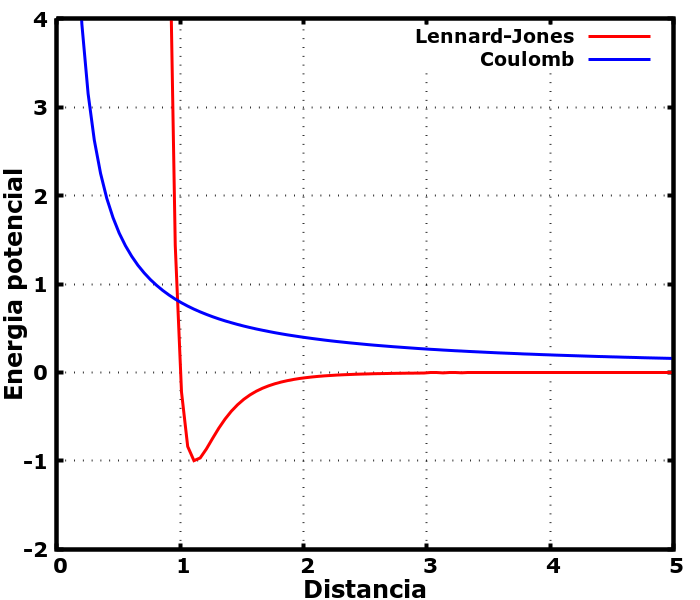
\includegraphics[width=\textwidth]{poten.png}
\caption{Curvas do potencial de Lennard-Jonnes e Coulombiano. As propriedades estão em unidades arbitrárias. Os parâmetros (ver Equação \ref{FF}) $\epsilon, \sigma, q_i \; \text{e} \; q_j$ foram definidos como a unidade e o $\epsilon_0$ como 0.1.}
\label{LJCOUL}
\end{figure}

Para que a força não seja avaliada de forma errada, já que não é possível considerar um raio de corte pequeno devido à forma do potencial eletrostático e nem um grande por causa da convenção de imagem mínima, algumas estratégias são descritas na literatura para contornar esse problema.
As interações de Lennard-Jones podem ser avaliadas com um raio de corte como descrito anteriormente.
Mas as interações eletrostáticas são de longo alcance, e devem ser calculadas com um algoritmo próprio para esse tipo de interação.
Aqui mostraremos uma das metodologias conhecida como \textit{Particle-Mesh-Ewald} (PME)\cite{Darden1993, Essmann1995}.
Nesse método, o somatório das interações eletrostáticas é resolvido para todas as réplicas geradas, para isso, mais um somatório é inserido varrendo todas as caixas de simulação existentes:

\begin{equation}
\begin{aligned}
V = \sum_n \sum_{i}^N \sum_{j>i}^N \frac{q_i q_j}{4\pi \epsilon_0} \frac{1}{r_{ij} + \mathbf{n}}
\end{aligned}
\end{equation}
onde $\mathbf{n}=L_x n_x + L_y n_y + L_z n_z$ é um vetor que varre todas as réplicas de caixas de simulação, $L_i$ é o comprimento da caixa de simulação no eixo $i$.

Esse somatório é de convergência condicional e, quando converge, lenta. 
A adoção de um raio de corte á ineficaz por motivos já discutidos anteriormente. 
A fim de efetuar a soma, essa série é dividida em duas  através da identidade\cite{Leach2001}:

\begin{equation}
\begin{aligned}
\frac{1}{r} = \frac{f(r)}{r} + \frac{1-f(r)}{r}
\end{aligned}
\end{equation}
de tal forma que a função $f(r)$ é escolhida para que as duas novas séries tenham uma boa convergência.

É reportado na literatura que uma boa escolha é a função erro complementar: $f(r) = erfc(\beta |r+n|)$.
Assim, pode-se resolver o primeiro termo no espaço real e o segundo em uma malha no espaço recíproco, onde $\beta$ controla quanto da interação será resolvida em cada um dos espaços.
Na prática, ele é um parâmetro ajustado para otimização de esforço computacional.
Dessa forma, a expressão de fato resolvida são duas séries de rápida convergência\cite{Darden1993, Essmann1995}:

\begin{equation}
\begin{aligned}
V = \sum_n \sum_{i}^N \sum_{j>i}^N \frac{q_i q_j}{4\pi \epsilon_0} \frac{erfc(\beta |r_{ij}+\mathbf{n}|)}{|r_{ij} + \mathbf{n}|} + \frac{1}{\pi V} \sum_{m \neq 0} \frac{exp(-\pi^2 \mathbf{m}^2/\beta)}{\mathbf{m}^2}exp(2\pi i \mathbf{m} * \mathbf{r})
\end{aligned}
\end{equation}
onde $\mathbf{m}$ é o vetor que varre o somatório em todas as réplicas no espaço recíproco e $V$ é o volume da caixa de simulação.

\section{PyPolyBuilder}\label{PyPolyBuilder}
O PyPolyBuilder é um software que está sendo desenvolvido no nosso grupo com o objetivo de facilitar a criação de topologia e coordenadas iniciais de moléculas poliméricas, em especial dendrímeros, para simulação por dinâmica molecular.
Como o aumento do número de átomos cresce exponencialmente com o aumento da geração dos dendrímeros, rapidamente a geração de um arquivo de topologia manualmente se torna inviável (Ver Tabela \ref{tab:pypolybuilder}).
Por isso, é justificada a criação de um software que automatize esse processo.
Aliado à isso, foi feita uma generalização para a criação de estruturas poliméricas em geral.
O software funciona baseado em dois módulos.
O módulo \textit{dendrimer} que é otimizado para a geração de dendrímeros e torna o processo muito mais fácil e o módulo \textit{general} que é generalizado e possibilita a criação de qualquer estrutura polimérica dependendo somente da criatividade do usuário.
Ele se baseia em pequenos blocos de construção que se repetem ao longo da estrutura da molécula desejada e os replica um determinado numero de vezes pedido pelo usuário.
Buscando simplificar o seu uso, um pequeno número de variáveis devem ser definidas pelo usuário na chamada do programa, são elas:
($i$) Nomes dos arquivos dos blocos de construção;
($ii$) arquivo com parâmetros do campo de força;
($iii$) o nome dos arquivos de saída é opcional, mas pode ser definido e
($iv$) o número da geração do dendrímero desejado (no caso do módulo \textit{dendrimer}) ou o arquivo com as ligações entre os blocos (no caso do módulo \textit{general}).

\begin{table}[ht!]
\centering
\caption{Tabela mostrando o aumento do número de átomos com o aumento da geração para dendrímeros PAMAM e PPI em meio com alto pH.}
\begin{tabular}{cc|cc}
\hline
\multicolumn{2}{c|}{PAMAM}   & \multicolumn{2}{c}{PPI} \\
\hline
G & \#Átomos& G & \#Átomos \\
\hline
0 & 48      & 1 &   30\\
1 & 128     & 2 &   70\\
2 & 288     & 3 &   150\\
3 & 608     & 4 &   310\\
4 & 1248    & 5 &   630\\
5 & 2528    & 6 &   1270\\
\hline
\end{tabular}
\label{tab:pypolybuilder}
\end{table}

Como ele é desendolvido em python, o PyPolyBuilder pode ser facilmente utilizado em qualquer computador.
Devido à algumas dificuldades na geração de coordenadas iniciais para o módulo \textit{general} e pela falta de uma validação sistemática até a presente data, o código ainda não foi publicado.


\subsection{Módulo \textit{Dendrimer}}

\begin{figure}[ht!]
\centering
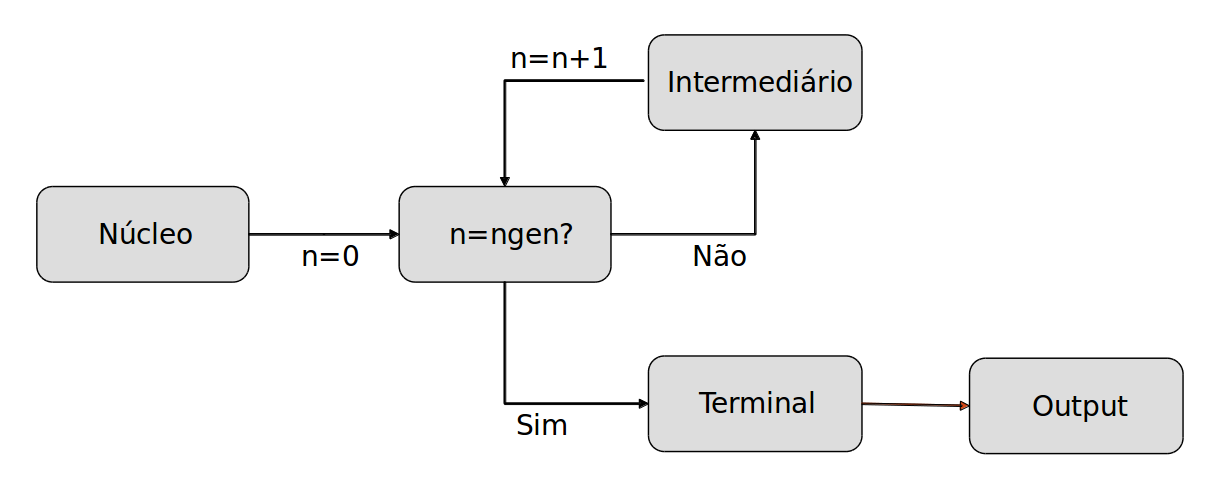
\includegraphics[width=\textwidth]{PyPolyBuilderDend}
\caption{Fluxograma ilustrativo do funcionamento do módulo \textit{dendrimer} do PyPolyBuilder.
O \textit{software} parte do bloco nuclear e compara a geração do dendrímero com a geração pedida pelo usuário. 
Enquanto ele não alcançar o número de geração pedido, uma nova camada de blocos intermediários é conectada.
Quando o tamanho desejado é obtido, uma camada de blocos terminais é conectado e os arquivos de saída são gerados.}
\label{fig:PyPolyBuilderDend}
\end{figure}

O módulo especializado para a geração de dendrímeros usa a simetria da molécula para automatizar a ligação entre os blocos de construção.
Nesse módulo, o usuário precisa fornecer a topologia dos blocos de construção do núcleo, intermediário e terminal, o arquivo de parâmetros do campo de força e o número de geração desejado.
Assim, o PyPolyBuilder parte do núcleo e conecta blocos terminais, camada por camada, até que a geração alcance o valor desejado.
Então os blocos terminais são conectados e a geometria tri-dimensional é gerada seguindo algumas heurísticas.
O usuário pode pedir para uma otimização de geometria ser feita.
Os arquivos de saída (topologia e coordenadas) são escritos em um formato compatível com o software Gromacs\cite{VanDerSpoel2005}.
O fluxograma do programa é exibido na Figura \ref{fig:PyPolyBuilderDend}.


\subsection{Módulo \textit{General}}

\begin{figure}[ht!]
\centering
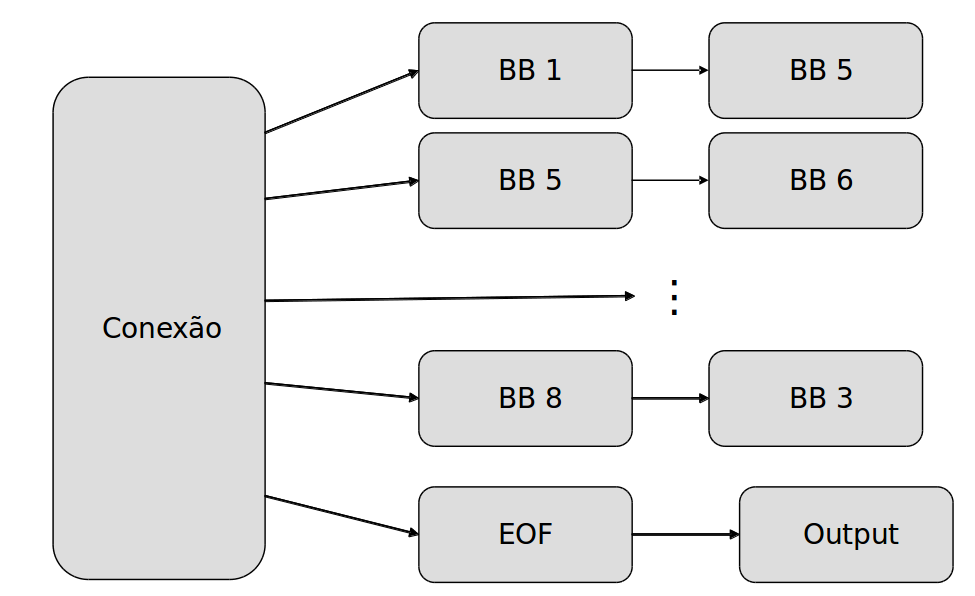
\includegraphics[width=\textwidth]{PyPolyBuilderGen}
\caption{Fluxograma ilustrativo do funcionamento do módulo \textit{general} do PyPolyBuilder.
A partir do arquivo de conexões fornecido pelo usuário, o PyPolyBuilder conecta os blocos de construção através dos átomos passados, também, pelo arquivo de conexão.
Ao chegar no final do arquivo, os arquivos de saída são gerados.}
\label{fig:PyPolyBuilderGen}
\end{figure}

Já no módulo geral, diferentemente do otimizado para dendrímeros, nenhuma geometria é pressuposta.
Por isso, ao invés de um único escalar para reger seu tamanho, um arquivo de conexões é necessário.
Nesse arquivo, a cada linha deve ser definido os índices de quais blocos devem se ligar e dos dois átomos que serão utilizados para a formação da ligação química.
O PyPolyBuilder lê essa lista enquanto cria a topologia e ao chegar no fim do arquivo, ele escreve a saída em arquivo.
O Fluxograma está ilustrado na Figura \ref{fig:PyPolyBuilderGen}.

Além do arquivo de conexões, as topologias de cada um dos blocos de construção utilizados devem ser fornecidas e, também, o arquivo contendo os parâmetros do campo de força.
Esse módulo foi satisfatoriamente utilizado para a geração de \textit{Hyper Branched Polymers} (HBP) propostos por Yu \textit{et al}\cite{Yu2016} em seu \textit{HBP Builder}.
Contudo, a abordagem do PyPolyBuilder é completamente determinística, diferentemente da geração estocástica do \textit{HBP Builder}.

\section{Propriedades}\label{Propriedades}

\subsection{Raio de giro}\label{RaioDeGiro}
O raio de giro médio quadrático nos fornece uma descrição quantitativa do tamanho de uma macromolécula.
Essa é uma propriedade amplamente conhecida e utilizada na ciência de polímeros e tem sido comumente utilizada, também, para a caracterização de dendrímeros. 
Para uma molécula com N átomos:

\begin{equation}
\langle R_g^2 \rangle  = \frac{1}{M} \Bigg \langle\sum_{i=1}^{N} [{m_i}(|\vec{r}_i-\vec{R}|^2)] \Bigg \rangle,
\end{equation}
onde, M é a massa total da molécula, $m_i$ é a massa do átomo i, $\textbf{r}_i$ o vetor de coordenadas do átomo i, $\textbf{R}$ é o vetor de coordenadas do centro de massa da molécula.

Foi feita uma análise avaliando a influência de se determinar o $R_g$ utilizando o centro de massa do bloco central ou do dendrímero como um todo. Como o principal objetivo deste trabalho é a validação do campo de força, foi decidido calcular o raio de giro com base no centro de massa do dendrímero completo já que essa é a forma mais comumente utilizada nos trabalhos encontrados na literatura.

\subsection{Asfericidade}\label{Fator de forma}\label{Asfericidade}
A forma dos dendrímeros é comumente avaliada com base nas razões de aspecto e no valor de asfericidade do mesmo, que dão uma ideia do quão esférico é a forma da molécula avaliada.

Para isso, obtemos os valores dos momentos de inércia (I) através do cálculo dos autovalores do tensor de forma ($\mat{G}$) e convencionando que $I_z > I_y > I_x$: \cite{Rapaport2005}

\begin{equation}
 \mat{G}_{mn} = \frac{1}{M} \sum_{i=1}^{N} [{m_i}(r_{mi}-{R_m})(r_{ni}-{R_n})]
\end{equation}
onde $m,n = x,y,z$, M é a massa total da molécula, $m_i$ é a massa do átomo i, $\textbf{r}_i$ o vetor de coordenadas do átomo i, $\textbf{R}$ é o vetor de coordenadas do centro de massa da molécula.

As razões de aspecto são frações envolvendo os momentos de inércia de diferentes eixos.
Essas relações mostram o quanto a projeção da molécula no plano envolvendo os eixos escolhidos divergem de um círculo, ou seja, quanto mais distante da unidade for a razão de aspecto, menos circular é a projeção da molécula naquele plano.
As razões de aspecto calculadas foram:

\begin{equation}
\frac{I_z}{I_y} \quad \text{e} \quad \frac{I_z}{I_x}
\end{equation}

Enquanto a asfericidade é obtida através da equação proposta por Rudnick e Gaspari\cite{rudnick1986}:

\begin{equation}
\delta = 1 - 3\frac{\langle I_2 \rangle}{\langle {I_1}^2 \rangle};
\end{equation}
onde $I_1 = I_x + I_y + I_z$ and $I_2 = {I_x}{I_y}+{I_x}{I_z}+{I_y}{I_z}$.

Nessa abordagem, quão mais esférica for a molécula, mais próximo de zero estará o valor de $\delta$.

\subsection{Funções de distribuição radial}\label{RDF}
As funções de distribuição radial (RDF) medem o número médio de átomos do tipo $\beta$ a uma distância r de átomos do tipo $\alpha$ dividido pelo número que um gás ideal de mesma densidade teria na mesma distância r.\cite{Allen2017}
Para que essa função seja avaliada computacionalmente, a distância r é discretizada em camadas de espessura $\Delta r$ e o número médio de átomos do tipo $\beta$ é contado dentro de cada esfera concêntrica ao redor dos átomos $\alpha$\cite{Allen2017}:

\begin{equation}
g_{\alpha\beta}(r) = (4\pi r^2\rho\Delta r)^{-1} \langle N_{\alpha\beta}(r; \Delta r) \rangle ,
\end{equation}
onde, $\rho$ é a densidade do meio, $\Delta r$ é a espessura considerada para a discretização do espaço e $\langle N_{\alpha \beta}(r;\Delta r) \rangle$ é o número médio de átomos do tipo $\beta$ dentro do intervalo $(r-\nicefrac{\Delta r}{2}, r+\nicefrac{\Delta r}{2})$ de um átomo do tipo $\alpha$.

Esses perfis radiais nos fornecem informação sobre como é a dispersão local de um grupo de átomos $\beta$ em relação à um grupo de átomos $\alpha$. 
As RDFs são também chamadas de perfis de densidade radial por avaliarem uma dendidade numérica relativa em relação à um meio ideal. Porém, não é raro encontrarmos curvas onde a função de distribuição radial não é normalizada pelo volume da casca esférica considerada. 
Esse tipo de análise é comum quando queremos o número absoluto de átomos do tipo $\beta$ dispersos ao redor de $\alpha$.


\chapter{Metodologia}
\section{Sistemas simulados}\label{SistemasSimulados}

Simulações de dinâmica molecular foram efetuadas utilizando os dendrímeros Poli(amido amina) (PAMAM) com núcleo de etileno diamina (EDA) e Poli(propileno imina) (PPI) com núcleo de 1,4-diamino butano (DAB) de gerações 0 até 5 e 1 à 6, respectivamente, considerando condições de pH alto($pH > 10.0$), neutro($pH \sim 7.1$) e baixo($pH < 4.0$).
A tabela \ref{tab:sistemas} reporta os 36 sistemas simulados explicitando o número de átomos no dendrímero, de contra-íons e de moléculas de solvente.

A escolha de uma faixa diferente de gerações para o PAMAM e o PPI (também conhecido como Astramol\cite{Kabanov1999}) é devido à nomenclatura utilizada pela literatura para cada um dos dendrímeros ser distinta.
As gerações foram escolhidas de forma que houvessem o mesmo número de grupos terminais para ambas as estruturas.

\begin{table}[ht]
\centering
    \begin{tabular}{ccccc|ccccc}
    \hline
    \multicolumn{5}{c|}{PAMAM} & \multicolumn{5}{c}{PPI} \\
    \hline
    Gen.    &  pH  &    \#Atoms    &    \#Cl$^{-}$ &    \#Water & Gen.      &  pH  &    \#Atoms    &    \#Cl$^{-}$ &    \#Water    \\
    \hline
    G0  &  \multirow{6}{*}{Low}  &   54      &   6   &   1674    & G1     &  \multirow{6}{*}{Low}&   36      &   6   &   1348\\
    G1  &    &   142     &   14  &   4292    & G2     &  &   84      &   14  &   2921\\
    G2  &    &   348     &   30  &   11803   & G3     &  &   180     &   30  &   5257\\
    G3  &    &   670     &   62  &   10394   & G4     &  &   372     &   62  &   8486\\
    G4  &    &   1374    &   126 &   19248   & G5     &  &   756     &   126 &   13075\\
    G5  &    &   2782    &   254 &   36214   & G6     &  &   1524    &   254 &   23546\\
    \hline 
    G0  &  \multirow{6}{*}{Neutral} &    52      &   4   &   1666    & G1     &  \multirow{6}{*}{Neutral}&   34      &   4   &   1140\\
    G1  &  &    136     &   8   &   4033    & G2     &  &    78      &   10  &   2416\\
    G2  &  &    304     &   16  &   8550    & G3     &  &    172     &   22  &   3593\\
    G3  &  &    640     &   32  &   13241   & G4     &  &    356     &   46  &   5014\\
    G4  &  &    1312    &   64  &   17982   & G5     &  &    724     &   94  &   9723\\
    G5  &  &    2656    &   128 &   34096   & G6     &  &    1460    &   190 &   14865\\
    \hline
    G0  &  \multirow{6}{*}{High}&   48      &   0   &   1348    & G1     &  \multirow{6}{*}{High}&    30      &   0   &   1143\\
    G1  &  &   128     &   0   &   3653    & G2     &  &   70      &   0   &   1482\\
    G2  &  &   288     &   0   &   8281    & G3     &  &   150     &   0   &   2258\\
    G3  &  &   608     &   0   &   15943   & G4     &  &   310     &   0   &   3213\\
    G4  &  &   1248    &   0   &   14713   & G5     &  &   630     &   0   &   4136\\
    G5  &  &   2528    &   0   &   23565   & G6     &  &   1270    &   0   &   6351\\
    \hline
    \end{tabular}
    \caption{Dimensões dos sistemas considerados nesse trabalho. O número de íons Cl$~{-}$ reportados para o PPI nessa tabela foram calculados considerando a protonação de acordo com o modelo de Ising\cite{VanDuijvenbode1998, Koper1997}.}
    \label{tab:sistemas}
\end{table} 

As condições de pH foram levadas em conta considerando os estados de protonação propostos por Cakara \textit{et al}\cite{Cakara2003}: Em pH ácido, todas as aminas estão protonadas; em neutro, somente as primárias e em pH baixo nenhuma delas é protonada. 
A Figura \ref{PAMAMProt} ilustra o esquema de protonação utilizado para o PAMAM.
Contudo, ainda não existe um acordo sobre o perfil de protonação do PPI na literatura. 
Por isso, dois estados de protonação diferentes foram considerados para o meio com pH neutro: Um deles supondo uma protonação idêntica à do PAMAM (somente os terminais protonados) e outra considerando que somente a penúltima geração estaria desprotonada, como proposto por trabalhos baseados no modelo de Ising\cite{VanDuijvenbode1998, Koper1997} (Essa ultima será referenciada na Tabela \ref{tab:Rg} como ``NEWPROT'' na Seção \ref{ProtonacaoPPI}).
Resultando em um total de 42 simulações efetuadas.

\begin{figure}[ht]
\centering
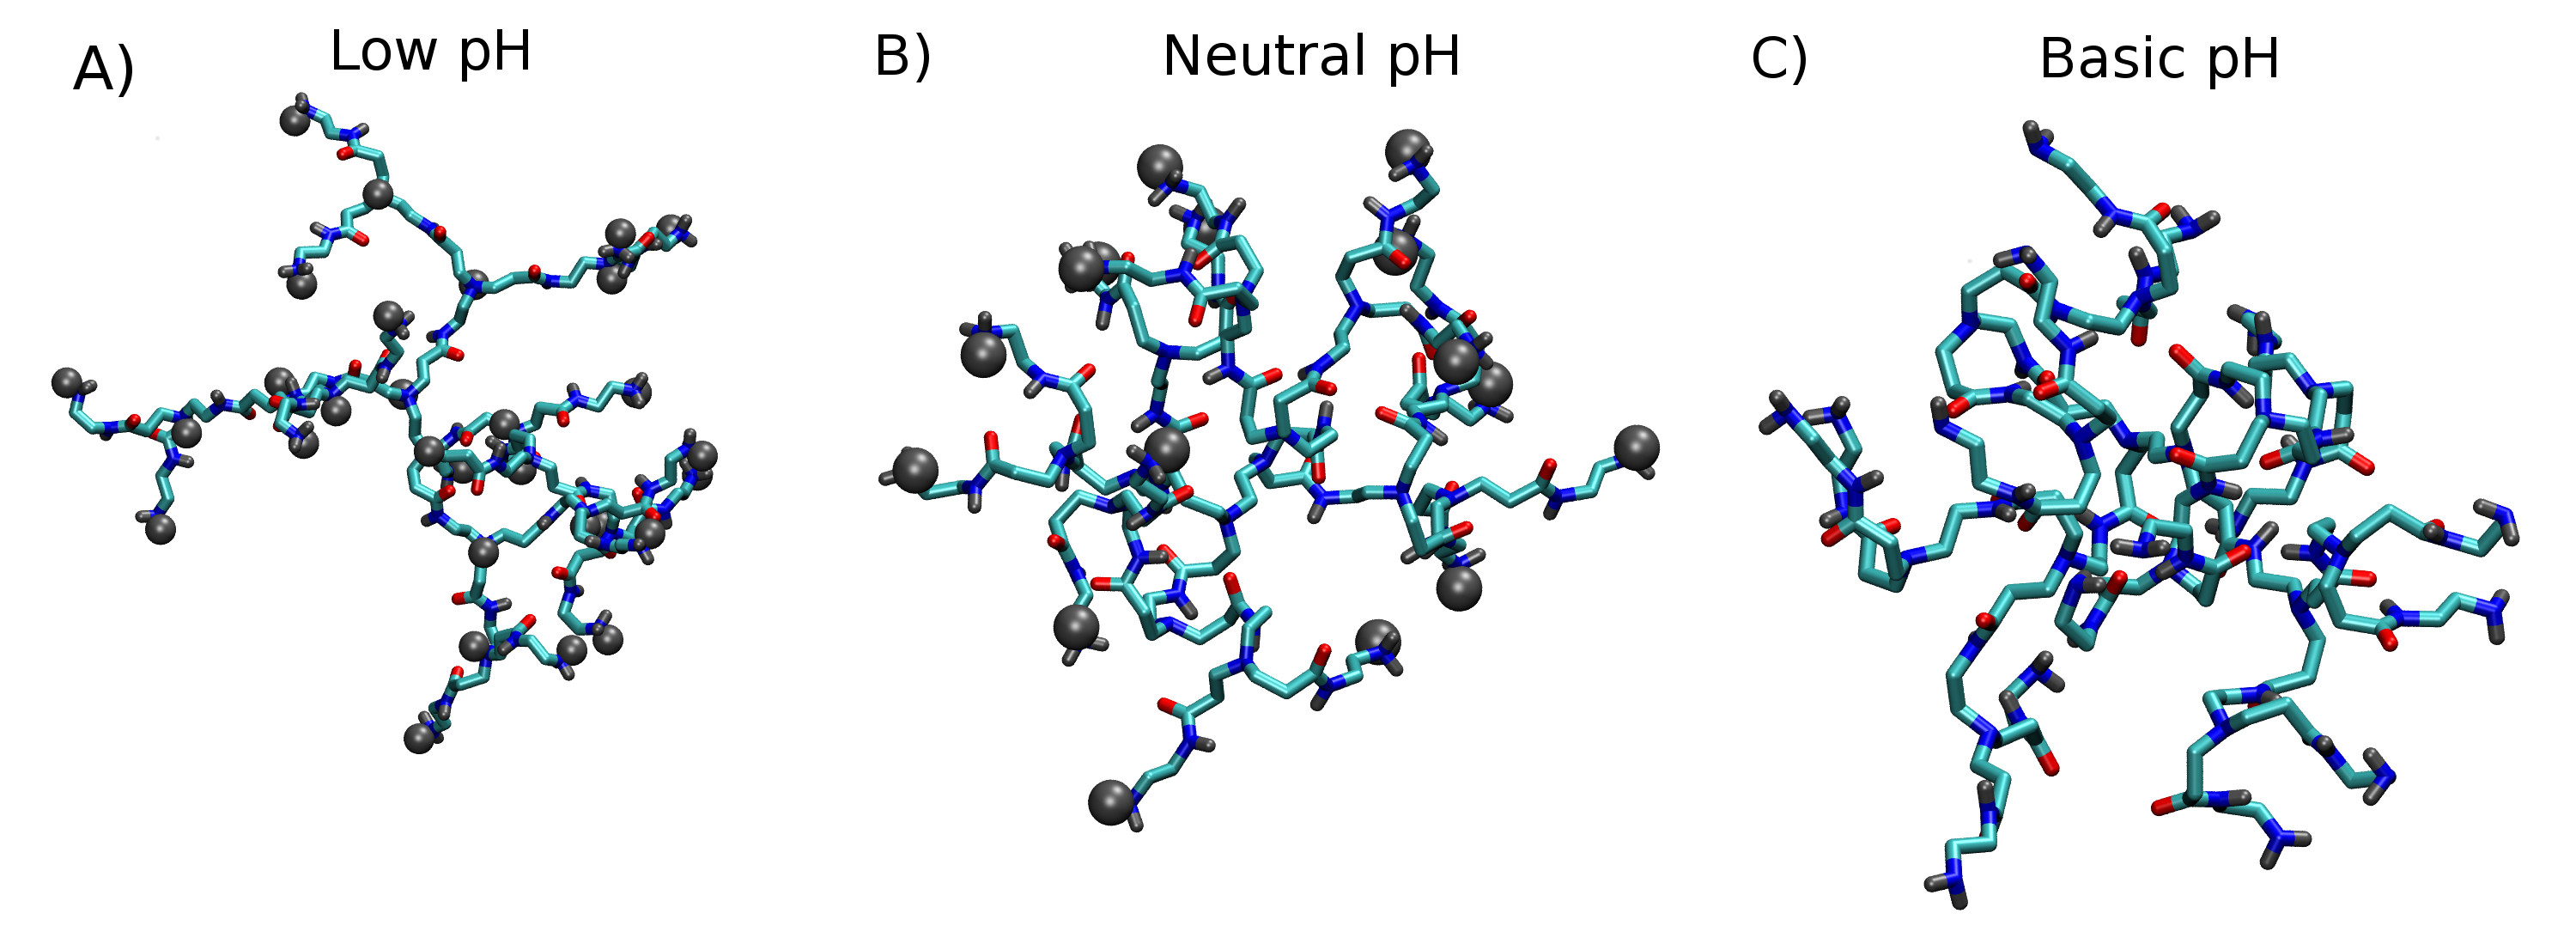
\includegraphics[scale=0.15]{PAMAMProt.png}
\caption{Esquema de protonação do PAMAM de terceira geração. As esferas de van der Waals em cinza representam os hidrogênios inseridos devido ao pH do meio.}
\label{PAMAMProt}
\end{figure}

De fato, o modelo utilizado como base não é determinístico. 
Ele resulta em um grau de protonação dado em percentual do sítio estar protonado ou não.
O estado de protonação sugerido pelos autores\cite{VanDuijvenbode1998, Koper1997} foi um onde cada geração é protonada intercaladamente.
Ou seja, ou todas as gerações pares estarão protonadas ou todas as ímpares.
Isso se deve ao fato de que a protonação de um sítio causa uma repulsão que impede a aproximação de prótons nos sítios de gerações vizinhas.
Mas como o resultado é probabilístico, as curvas de grau de protonação em função do pH estão próximas de 0.5 no estudo reportado\cite{VanDuijvenbode1998, Koper1997}.
Por isso o estado de protonação escolhido foi distinto do proposto no trabalho original aqui citado.
Contudo, veremos à frente que em termos de raio de giro, a diferença não é significativa.

As estruturas iniciais e as topologias foram criadas utilizando o software PyPolyBuilder, criado pelo nosso grupo.
Esse programa se propõe a criar arquivos de estrutura e de topologia para moléculas a partir de blocos de construção menores como foi exposto na Seção \ref{PyPolyBuilder}.


\section{Protocolo de simulação}\label{ProtocoloDeSimulacao}
As simulações de todos os 42 sistemas foram efetuadas utilizando o pacote GROMACS 5.1.4\cite{VanDerSpoel2005} e o campo de força GROMOS-compatible 2016H66\cite{Horta2016}.
As equações de Newton foram integradas usando o algoritmo leap-frog com passo de tempo de 2 fs.
Todas as ligações foram mantidas rígidas segundo o algoritmo LINCS\cite{Hess1997}.
As interações eletrostáticas foram avaliadas com o método PME\cite{Essmann1995} com um raio de corte do espaço real de $1.2$ nm e um espaçamento de malha de $0.12$ nm.

Dois \textit{setups} foram considerados para as interações de Lennard-Jones para avaliar a influência das configurações da simulação utilizando o campo de força 2016H66\cite{Horta2016} no GROMACS, segundo a filosofia do estudo de Gonçalves \textit{et al}\cite{Goncalvez2018}. 
Em uma delas, nomeada de ``CUT'', as interações foram truncadas em $1.2$ nm usando um raio de corte simples, método conhecido como \textit{cut-off}.
Em outra, rotulada como ``PME'', avaliamos as interações segundo o método PME\cite{Essmann1995} com raio de corte do espaço real de $1.2$ nm e espaçamento de malha de $0.12$ nm.
Veremos na Seção \ref{EfeitoDoSetup} que nos sistemas considerados na presente dissertação, a escolha do \textit{setup} não teve grande efeito.
Os resultados são praticamente os mesmos independentemente do método de avaliação das interações de Lennard-Jones.

Vale notar que o protocolo descrito acima não está de acordo com a parametrização do campo de força, mas foi mostrado ser o mais adequado em um estudo sistemático realizado por Gonçalves \textit{et al}\cite{Goncalvez2018}.

Temperatura e pressão foram controladas por acoplamento fraco com um banho externo de calor e de volume segundo o termostato modificado de Berendsen\cite{Berendsen1984, Bussi2007} e o formalismo de Parrinelo-Rahman\cite{Parrinello1981, Andersen1980}, respectivamente.
A constante de tempo do acoplamento térmico foi definida como 0.1 ps e, para o acoplamento de pressão, a constante de tempo e a compressibilidade isotérmica utilizadas foram 2.0 ps e $4.5\times10^{-5}$bar$^{-1}$, respectivamente.

Primeiramente, uma minimização em vácuo foi realizada por 5000 passos e o sistema foi colocado em uma caixa de simulação cúbica de forma que todos os átomos estivessem, no mínimo, a $1$ nm de distância das faces dessa caixa.
O sistema foi então solvatado com uma quantidade suficientemente grande de moléculas de água SPC\cite{Berendsen1981}.
Nos casos onde a carga total do sistema não fosse neutra, o sistema foi neutralizado pela adição de contra-íons Cl$^{-}$ (para mais informações, veja a Tabela \ref{tab:sistemas}).
Após a solvatação, uma nova etapa de minimização de energia foi feita considerando condições de contorno periódicas.

\begin{figure}[ht]
\centering
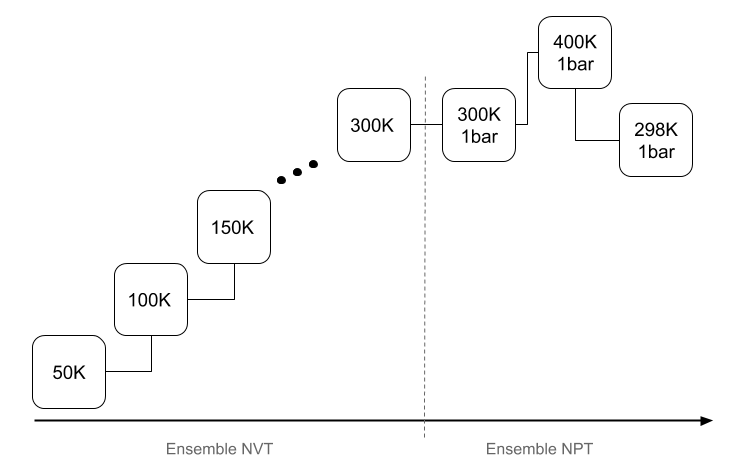
\includegraphics[scale=0.6]{equilib.png}
\caption{Rampa de temperatura considerada para a equilibração do sistema. Cada um dos ciclos foi simulado por 200 ps.}
\label{equilib}
\end{figure}

A equilibração dos sistemas foi realizada em um ensemble NVT onde a temperatura foi elevada gradadivamente segundo um perfil de escada para evitar uma movimentação que pudesse levar à superposições de volumes atômicos e consequente divergência do sistema.
Velocidades iniciais foram geradas segundo uma distribuição de Maxwell-Boltzmann correspondente à temperatura de 50K.
Então, seis equilibrações sucessivas de 200 ps foram realizadas aumentando gradualmente a temperatura de 50 a 300 K em intervalos de 50K (Figura \ref{equilib}).
Após isso, a equilibração foi continuada no ensemble NPT controlando a pressão em 1 bar.
A fim de remover influências da estrutura inicial, o sistema foi levado até 400K e simulado por 200 ps antes de ser resfriado a 298.15 K por mais 200 ps (Figura \ref{equilib}).
Essa equilibração lenta é particularmente importante para os dendrímeros de gerações mais altas devido a sua estrutura altamente complexa.

Após a equilibração, 50 ns de dinâmica molecular foram feitos com a configuração descrita acima. 
Para garantir que as propriedades fossem calculadas em uma janela de tempo onde elas já haviam convergido, os últimos 10 ns foram utilizados para o cálculo das propriedades para a validação e estudo dos sistemas.
O raio de giro e as funções de distribuição radial foram calculadas com rotinas nativas do gromacs-5.1.4 enquanto os fatores de forma e as asfericidades, com um script escrito pelos autores por motivos que serão melhor discutidos nas Seções \ref{PAMAMForma} e \ref{PPIForma}.

\pagebreak


\chapter{Resultados e discussão}\label{Resultados}

\section{Efeito do \textit{setup} das simulações}\label{EfeitoDoSetup}

\subsection{Interações de Lennard-Jones}

A Tabela \ref{tab:Rg} contém os valores dos raios de giro calculados para ambos os \textit{setups} considerados na Seção \ref{ProtocoloDeSimulacao}. 
Nas colunas ``PME'' e ``CUT'' os erros absolutos são da ordem de $0.01$ nm. 
Logo, conclui-se que a mudança do algoritmo para avaliação das interações de Lennard-Jones não afeta o raio de giro.

Claro que diferentes distribuições de partículas podem gerar o mesmo raio de giro para diferentes estruturas.
Mas a análise de funções de distribuição radial também não revelou alterações significativas frente a mudança do algoritmo de avaliação.

Visto isso, somente serão apresentados os resultados obtidos utilizando o método do \textit{cut-off} com raio de corte de $1.2$ nm, que é a configuração ótima obtida pelo trabalho de Gonçalvez \textit{et al}\cite{Goncalvez2018} em um estudo muito mais abrangente e sistemático na avaliação de configurações de simulação utilizando o 2016H66\cite{Horta2016} no GROMACS\cite{VanDerSpoel2005}.
As curvas utilizando o método PME são mostradas nos apêndices \ref{PAMAMap} e \ref{PPIap}.

%\begin{landscape}
\begin{table}[ht!]
\centering
\begin{tabular}{c|ccc|cccc}
\hline
  Environment   & \multicolumn{3}{c|}{PAMAM} & \multicolumn{4}{c}{PPI} \\
\hline
\multirow{2}{*}{pH}    & \multirow{2}{*}{G} &   This work & This work & \multirow{2}{*}{G} & This work & This work & This work  \\
&                               &   (PME)       &   (CUT)   &                               &   (PME)   &   (CUT)  &   (NEWPROT) \\
\hline
\hline
\multirow{6}{*}{Low} & 0    &   0.58  &   0.59  & 1 &  0.51  &   0.51  &   - \\
                        & 1    &   1.01  &   1.00  & 2 &  0.78  &   0.79  &   - \\
                        & 2    &   1.47  &   1.48  & 3 &  1.04  &   1.06  &   - \\
                        & 3    &   1.91  &   1.97  & 4 &  1.34  &   1.35  &   - \\
                        & 4    &   2.45  &   2.46  & 5 &  1.65  &   1.65  &   - \\
                        & 5    &   2.99  &   2.97  & 6 &  1.99  &   2.00  &   - \\
\hline
\multirow{6}{*}{Neutral}& 0 &   0.51  &   0.50  & 1 &  0.51  &   0.49  &   0.51 \\
                        & 1    &   0.79  &   0.79  & 2 &  0.77  &   0.76  &   0.77 \\
                        & 2    &   1.06  &   1.06  & 3 &  1.04  &   1.01  &   1.05 \\
                        & 3    &   1.45  &   1.45  & 4 &  1.34  &   1.30  &   1.33 \\
                        & 4    &   1.84  &   1.99  & 5 &  1.65  &   1.60  &   1.65 \\
                        & 5    &   2.53  &   2.51  & 6 &  1.98  &   1.91  &   1.98 \\
\hline
\multirow{6}{*}{High} & 0   &   0.49  &   0.48  & 1 &  0.49  &   0.49  &   - \\
                        & 1    &   0.75  &   0.72  & 2 &  0.74  &   0.74  &   - \\
                        & 2    &   0.99  &   1.00  & 3 &  0.95  &   0.94  &   - \\
                        & 3    &   1.24  &   1.18  & 4 &  1.07  &   1.03  &   - \\
                        & 4    &   1.60  &   1.56  & 5 &  1.25  &   1.31  &   - \\
                        & 5    &   1.96  &   1.96  & 6 &  1.60  &   1.56  &   - \\
\hline
\end{tabular}
\caption{Raio de giro $R_g$ (nm) obtidos nesse trabalho. Comparação quantitativa entre as diferentes configurações consideradas para as simulações feitas.}
\label{tab:Rg}
\end{table}
%\end{landscape}


\subsection{Protonação do PPI}\label{ProtonacaoPPI}

Como discutido na Seção \ref{SistemasSimulados}, dois estados de protonação distintos foram considerados para tratar o PPI em meio com pH neutro. 
Pela última coluna da Tabela \ref{tab:Rg}, é possível notar que, considerando um grau de protonação maior que o sugerido pelo modelo de Ising\cite{VanDuijvenbode1998, Koper1997}, não há uma alteração significativa do raio de giro quando aminas terciárias no PPI são protonadas.
Essa estrutura foi, também, simulada utilizando ambos os protocolos de avaliação das interações de Lennard-Jones (\textit{cut-off} e PME).
Mas os resultados, assim como os discutidos na seção anterior, não apresentam diferenças significativas.
Por isso, somente os resultados utilizando \textit{cut-off} são apresentados para essa protonação na Tabela \ref{tab:Rg}.

Pela análise das funções de distribuição radial, pode-se notar que a distribuição de aminas primárias sofre uma leve alteração em gerações maiores.
A escolha do PPI de acordo com o modelo de Ising\cite{VanDuijvenbode1998, Koper1997}, leva a uma distribuição onde há uma menor densidade de aminas terminais no interior do dendrímero e, consequentemente, um maior acúmulo na região superficial.
Esse é o comportamento encontrado nas estruturas em meio ácido.
Como consideramos um estado de protonação mais próximo ao que seria quando em pH baixo, o comportamento naturalmente tendeu à uma distribuição em maior acordo com o meio.

Como somente o raio de giro é uma propriedade de validação quantitativa, ambos os modelos de perfis de protonação podem ser considerados adequados.
No entanto, considerando uma avaliação qualitativa da forma das funções de distribuição radial em relação à outros trabalhos computacionais e teóricos o modelo de Ising\cite{VanDuijvenbode1998, Koper1997} parece ser mais adequado. Os resultados mostrados na Seção \ref{PPIEstrutura} são os obtidos de acordo com o modelo de Ising\cite{VanDuijvenbode1998, Koper1997} por serem análises mais refinadas do que a simples suposição de protonação semelhar ao PAMAM.

Os resultados obtidos são apresentados abaixo e foram separados em duas seções: Uma para a discussão do PAMAM e outra para o PPI. Dessa forma, detalhes específicos de cada um dos dendrímeros poderão ser melhor discutidos.

\begin{landscape}
\begin{table*}[t] %PAMAM Rg Suplemmental info tables
\centering
\caption{Comparação do raio de giro $R_g$ (em nm) calculado na presente dissertação para o PAMAM com valores disponíveis na literatura.
Os resultados estão organizados de acordo com o pH do meio (baixo, neutro e alto), número da geração $GN$ (de G0 à G5) e método utilizado no tratamento das interações de Lennard-Jones (PME: Particle-Mesh Ewald e CUT: \textit{cut-off scheme} com raio de corte de $1.2$ nm).
Os resultados da literatura mostrados foram tirados dos seguintes estudos:
SAXS(Prosa1997)\cite{Prosa1997},
SAXS(Rathgeber2002)\cite{Rathgeber2002},
CVFF(Lee2002)\cite{Lee2002},
Dreiding(Maiti2004)\cite{Maiti2004},
Dreiding(Maiti2005)\cite{Maiti2005},
GAFF(Opitz2006)\cite{Opitz2006},
SANS(Porcar2008)\cite{Porcar2008},
GAFF(Maingi2012)\cite{Maingi2012},
CHARMM(Caballero2013)\cite{Caballero2013},
CHARMM and GROMOS(Kanchi2018)\cite{Kanchi2018},
GAFF(Barraza2018)\cite{Barraza2018}.}
\scalebox{0.8}{
\begin{tabular}{cccccccccccccccc}
\hline
G$N$ & \multirow{2}{*}{pH}    & \multicolumn{2}{c}{This work} &GAFF\cite{Maingi2012}&    Dreiding\cite{Maiti2005}  & Dreiding\cite{Opitz2006} &Dreiding\cite{Maiti2004}  & CVFF\cite{Lee2002}     & GAFF\cite{Barraza2018}    &CHARMM\cite{Caballero2013}        &CHARMM\cite{Kanchi2018}   &GROMOS\cite{Kanchi2018}   &     SANS\cite{Porcar2008} & SAXS\cite{Rathgeber2002} & SAXS\cite{Prosa1997}\\
PAMAM   &               &   PME &   CUT &   &  &    &   &   &   &   &   &   &   &   &   \\
%   PAMAM   &               &   PME &   CUT &   Maingi2012      &   Maiti2005               &   Opitz2006           &Maiti2004              &   Lee2002             &   Barraza2018         &   Caballero2013           &Kanchi2018             &Kanchi2018             &   Porcar2008      & Rathgeber2002     & Prosa1997         \\
\hline
\hline
G0    & \multirow{6}{*}{Low} & 0.58  & 0.59          &       -           & -                         &   -                   &-                      &   -                   &   -                   &-                          &-                      &-                      &   -               &   -               &   -\\
G1   &                          & 1.01  & 1.00      &       -           & -                         &   -                   &-                      &   -                   &   -                   &-                          &-                      &-                      &   -               &   -               &   -\\
G2  &                          & 1.47  & 1.48      &       -           & -                         &   1.24                &-                      &   1.66                &   -                   &-                          &-                      &-                      &   -               &   -               &   -\\
G3     &                          & 1.91  & 1.97      &       -           & -                         &   1.64                &-                      &   2.28                &   -                   &-                          &-                      &-                      &   1.704           &   -               &   -\\
G4    &                          & 2.45  & 2.46      &       -           & 1.90                      &   2.13                &-                      &   2.99                &   -                   &-                          &-                      &-                      &   2.158           &   -               &   -\\
G5   &                          & 2.99  & 2.97      &       -           & 2.48                      &   2.65                &-                      &   3.80                &   -                   &-                          &-                      &-                      &   2.6839          &   -               &   -\\
\hline
G0     & \multirow{6}{*}{Neutral} & 0.51  & 0.50      &       -           & -                         &   -                   &-                      &   -                   & 0.61                  &-                          &-                      &-                      &       -           &   0.4             &   -   \\
G1    &                          & 0.79  & 0.79      &       -           & -                         &   -                   &-                      &   -                   & 0.93                  &-                          &-                      &-                      &       -           &   0.79            &   -       \\
G2   &                          & 1.06  & 1.06      &       -           & -                         &   0.95                &-                      &   1.45                & 1.26                  &-                          &-                      &-                      &       -           &   1.18            &   -       \\
G3  &                          & 1.45  & 1.45      &   1.578           & -                         &   1.21                &-                      &   1.97                & 1.52                  &1.533                      &1.408                  &1.619                  &   1.666           &   1.509           &   1.58    \\
G4     &                          & 1.84  & 1.99      &   2.064           & 1.70                      &   1.49                &-                      &   2.67                &   -                   &2.104                      &-                      &-                      &   2.129           &   1.86            &   1.71    \\
G5    &                          & 2.53  & 2.51      &   2.532           & 2.22                      &   2.08                &-                      &   3.28                &   -                   &2.550                      &-                      &-                      &   2.641           &   2.307           &   2.41    \\
\hline
G0   & \multirow{6}{*}{High}    & 0.49  & 0.48      &       -           & -                         &   -                   & 0.493                 &   -                   & 0.58                  &-                          &-                      &-                      &       -           &   -               &   -       \\
G1  &                          & 0.75  & 0.72      &       -           & -                         &   -                   & 0.746                 &   -                   & 0.84                  &-                          &-                      &-                      &       -           &   -               &   -       \\
G2     &                          & 0.99  & 1.00      &       -           & -                         &   0.94                & 0.917                 &   0.84                & 1.01                  &-                          &-                      &-                      &       -           &   -               &   -   \\
G3    &                          & 1.24  & 1.18      &   1.227           & -                         &   1.16                & 1.123                 &   1.16                & 1.31                  &-                          &-                      &-                      &   1.619           &   -               &   -       \\
G4   &                          & 1.60  & 1.56      &   1.550           & 1.68                      &   1.42                & 1.450                 &   1.48                & -                     &-                          &-                      &-                      &   2.092           &   -               &   -   \\
G5  &                          & 1.96  & 1.96      &   1.900           & 2.03                      &   1.80                & 1.834                 &   1.83                & -                     &-                          &-                      &-                      &   2.586           &   -               &   -   \\
\hline
\end{tabular}}
\label{tab:PAMAMRgValidacao}
\end{table*}
\end{landscape}

\section{PAMAM}

\subsection{Tamanho}\label{PAMAMTamanho}
O raio de giro foi calculado de acordo com o descrito na Seção \ref{RaioDeGiro} para cada sistema PAMAM relatado na Seção \ref{SistemasSimulados} e na Tabela \ref{tab:sistemas}, ou seja, das gerações 0 à 5 em meios com pH ácido, neutro e básico.
Os valores mostrados nas curvas a seguir estão listados na Tabela \ref{tab:PAMAMRgValidacao}.
Nela se encontram tanto os raios de giro dos sistemas simulados nesse trabalho quanto os disponíveis na literatura experimental e de simulação utilizados para validação.

\begin{figure}[ht!]
\centering
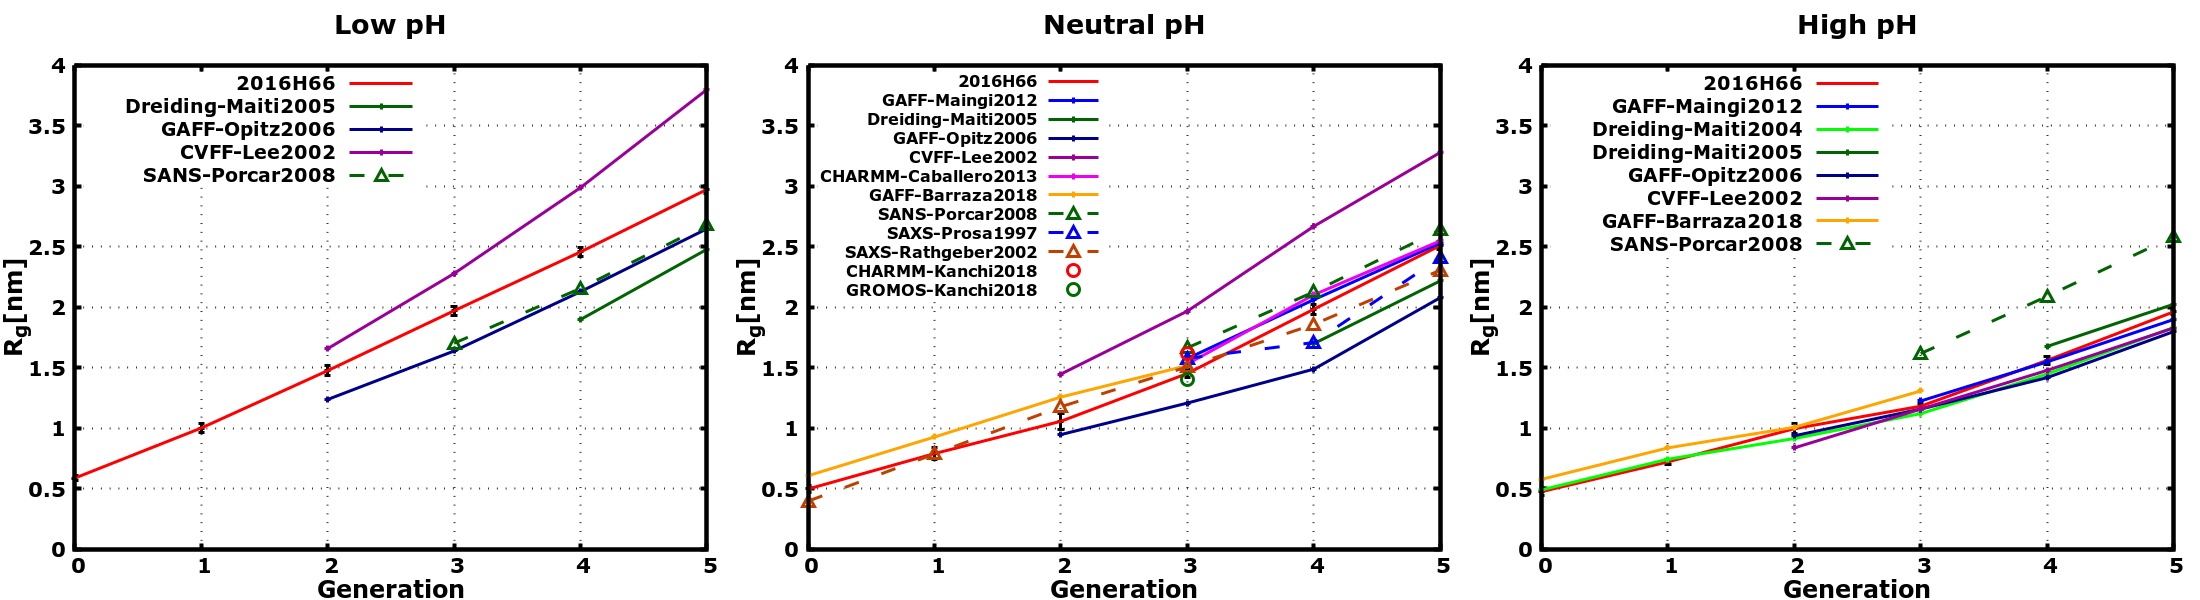
\includegraphics[width=\textwidth]{images/PAMAMRg.png}
\caption{Raio de giro ($R_g$) em função da geração em meios de pH baixo (imagem da esquerda), neutro (imagem do meio) e alto (imagem da direita).
Os resultados obtidos com o campo de força 2016H66\cite{Horta2016} são comparados com resultados de estudos experimentais e de simulações prévios:
Prosa1997\cite{Prosa1997}, %\cite{PR97.2},
Lee2002\cite{Lee2002}, %\cite{LE02.8},
Caballero2013\cite{Caballero2013}, %\cite{CA13.4},
Rathgeber2002\cite{Rathgeber2002}, %\cite{RA02.6},
Maiti2005\cite{Maiti2005}, %\cite{MA05.26},
Opitz2006\cite{Opitz2006}, %\cite{OP06.1},
Porcar2008\cite{Porcar2008}, %\cite{PO08.3},
Maiti2009\cite{Maiti2009}, %\cite{MA09.18},
Maingi2012\cite{Maingi2012}, %\cite{MA12.23},
Barraza2018\cite{Barraza2018}, %\cite{BA18.Y},
Kanchi2018\cite{Kanchi2018}.} %\cite{KA18.Y}.}
\label{fig:PAMAMRg}
\end{figure}


Quando em baixo pH, podemos ver que o 2016H66\cite{Horta2016} mantêm uma tendência quase linear assim como o resultado de espalhamento de neutrons a baixos ângulos (SANS) obtido por Porcar \textit{et al}\cite{Porcar2008}, mesmo que o 2016H66\cite{Horta2016} superestime os resultados consistentemente, em relação ao experimental.
Diferentemente, Lee \textit{et al}\cite{Lee2002} obtiveram um resultado que superestima consideravelmente o raio de giro de forma exponencial com o aumento da geração utilizando o campo de força CVFF\cite{Lifson1979} modelando o solvente implicitamente. 
Maiti \textit{et al}\cite{Maiti2005} conseguiram valores significativamente em acordo com os resultados reportados de SANS\cite{Porcar2008} utilizando o campo de força Dreiding\cite{Mayo1990} com moléculas de água e contra-íons explícitos no sistema.
Curiosamente, os resultados obtidos por Opitz e Wagner\cite{Opitz2006} revelaram um excelente acordo com os dados experimentais da literatura ao simular o PAMAM de gerações 2 a 5 usando metanol como solvente explicitamente. 

Em pH neutro, os resultados obtidos por Lee \textit{et al} continuam a superestimar exponencialmente todos os valores de raio de giro em relação aos estudos reportados na literatura, tanto experimental quanto de simulação.
Enquanto o estudo feito com o campo de força GAFF por Opitz e Wagner\cite{Opitz2006} subestima significativamente todos os outros resultados disponíveis na faixa de gerações estudada nesse trabalho.
O 2016H66\cite{Horta2016} está em excelente acordo com os resultados experimentais de SAXS reportados por Rathgeber \textit{et al}\cite{Rathgeber2002} e subestima um pouco os valores da propriedade quando comparados com o resultado de SANS reportados por Porcar \textit{et al}\cite{Porcar2008}, comportamento inverso do observado em baixo pH.
Os resultados de Prosa \textit{et al}\cite{Prosa1997} desviam fortemente do perfil quase linear apresentado pelos outros estudos disponíveis na literatura. Por isso, não existe um estudo que consistentemente esteja em acordo com os valores reportados por eles.
Podemos ver na imagem central da Figura \ref{fig:PAMAMRg} que em geração 3 os trabalhos com os campos de força CHARMM\cite{Caballero2013, Kanchi2018}, GAFF\cite{Maingi2012, Barraza2018}, 2016H66 (este trabalho) e até mesmo os resultados de SAXS\cite{Rathgeber2002} estão em bom acordo com os estudos de Prosa \textit{et al}\cite{Prosa1997}.
Mas em geração 4, podemos ver que somente o campo de força Dreiding \cite{Maiti2005} apresenta um bom acordo com ele.
Em relação à outros trabalhos de simulação, o 2016H66\cite{Horta2016} está em excelente acordo com os resultados de Maingi \textit{el al}\cite{Maingi2012} e de Caballero \textit{et al}\cite{Caballero2013} para as gerações de 3 à 5 (gerações disponíveis para comparação).
Especialmente para a geração 3, o 2016H66\cite{Horta2016} apresenta um excelente acordo com o valor reportado por Kanchi \textit{et al}\cite{Kanchi2018} para sua simulação utilizando o campo de força GROMOS86, trabalho no qual o autor mostra que esse campo de força foi o único capaz de reproduzir qualitativamente a superfície de energia livre de adsorção do dendrímero em uma membrana lipídica.

Já em alto pH, todos os trabalhos de simulação reportados estão relativamente de acordo, independentemente do campo de força e configurações utilizadas para o sistema.
E todos subestimam o raio de giro quando comparados com os resultados de SANS\cite{Porcar2008} disponíveis.

\begin{figure}[ht!]
\centering
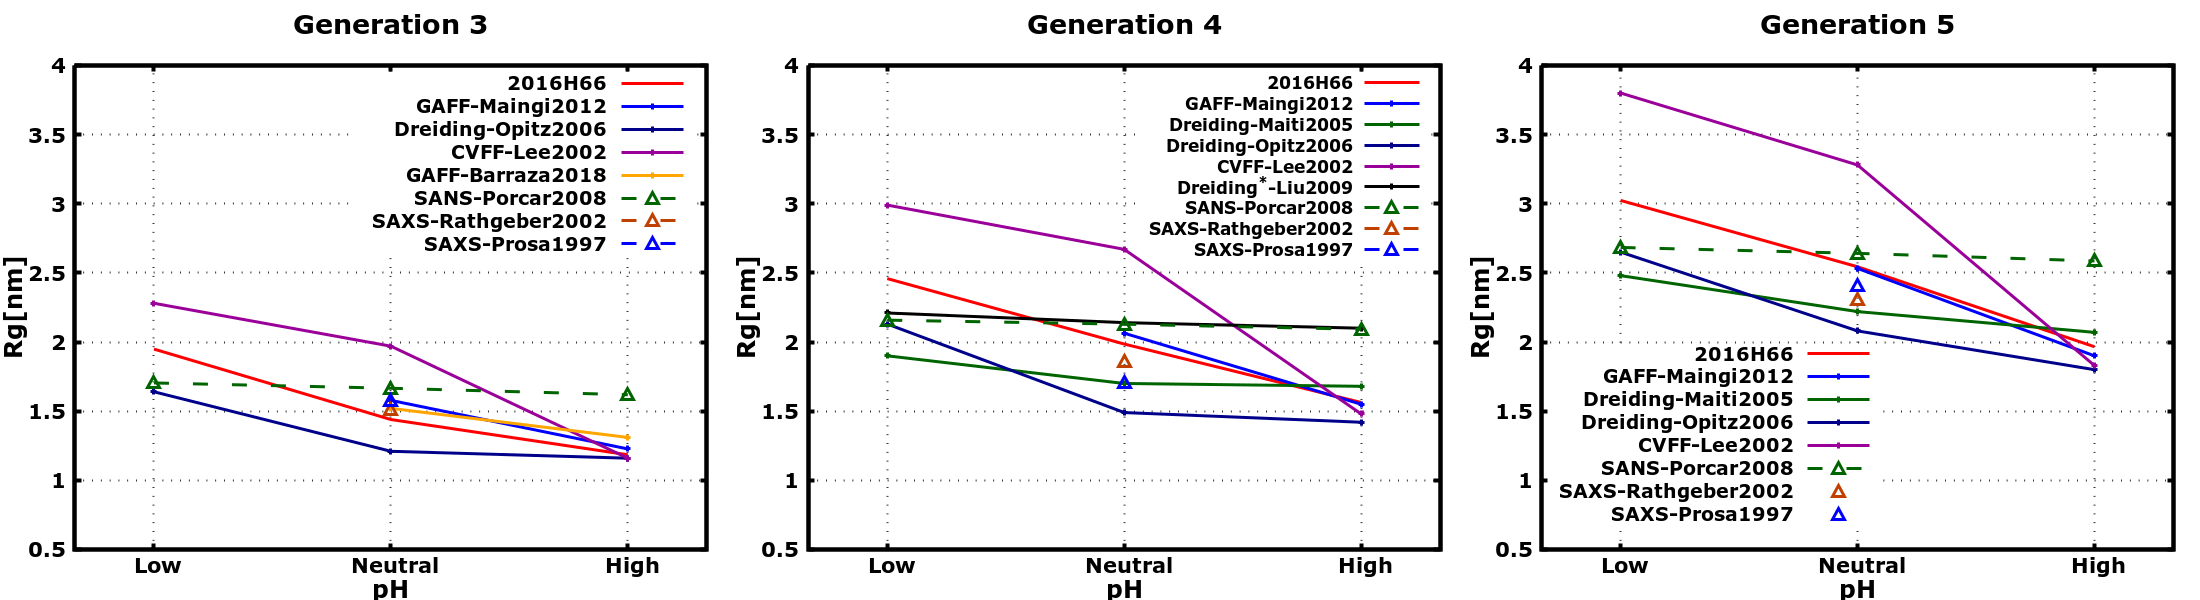
\includegraphics[width=\textwidth]{images/PAMAMgyrateGpH.png}
\caption{Raio de giro ($R_g$) em função do pH para o PAMAM de geração 3 (imagem da esquerda), 4 (imagem do meio) e 5 (imagem da direita).
Os resultados obtidos com o campo de força 2016H66\cite{Horta2016} são comparados com resultados de estudos experimentais e de simulações prévios:
Prosa1997\cite{Prosa1997}, %\cite{PR97.2},
Lee2002\cite{Lee2002}, %\cite{LE02.8},
Rathgeber2002\cite{Rathgeber2002}, %\cite{RA02.6},
Maiti2005\cite{Maiti2005}, %\cite{MA05.26},
Opitz2006\cite{Opitz2006}, %\cite{OP06.1},
Porcar2008\cite{Porcar2008}, %\cite{PO08.3},
Liu2009\cite{Liu2009}, %\cite{LI09.Y},
Maingi2012\cite{Maingi2012}, %\cite{MA12.23}.  }
Barraza2018\cite{Barraza2018}.} %\cite{BA18.Y},
\label{fig:PAMAMRgpH}
\end{figure}

Como foi discutido anteriormente, os valores obtidos com o campo de força 2016H66\cite{Horta2016} superestimam os resultados de SANS de Porcar \textit{et al}\cite{Porcar2008} em pH baixo e começam a subestimá-los em pH neutro e alto.
Esse comportamente se deve ao fato dos valores de SANS serem praticamente invariantes com o pH.
Como pode ser visto mais facilmente na Figura \ref{fig:PAMAMRgpH}, onde foi plotado os valores do raio de giro em função do pH para as gerações de 3 à 5.

A curva referente aos resultados de SANS\cite{Porcar2008} são constantes enquanto nas curvas de simulação os dendrímeros mostram um grande inchaço com o abaixamento do pH.
Esse resultado é esperado pois, devido a protonação de aminas terciárias internas, o aumento da repulsão eletrostática dá espaço para a entrada de moléculas de água na estrutura da molécula. 
O que, na prática, caracteriza o aumento das cavidades internas e, consequentemente, de toda a estrutura do dendrímero. Como discutido por Maiti e Goddard III\cite{Maiti2006} que simularam o PAMAM de geração 8 para comparar com o resultado de Nisato \textit{et al}\cite{Nisato2000}.
Resultados de SAXS\cite{Dootz2011} feitos em diferentes pHs relatam o acontecimento do inchaço característico do dendrímero.
Infelizmente, não há muitos estudos de SAXS em diferentes pHs para mostrar se esse comportamento é um artefato introduzido pela técnica de SANS ou pelo uso de modelos inadequados para a determinação do raio de giro em sistemas dendríticos.
A única exceção encontrada é o estudo de Liu \textit{et al}\cite{Liu2009} onde o PAMAM de geração 4 foi simulado em pH neutro e o resultado obtido está em total acordo com os dados de SANS\cite{Porcar2008}.
Porém, nesse trabalho Liu \textit{et al} precisaram introduzir um termo extra ao campo de força Dreiding que foi atribuído às ligações de hidrogênio tratadas de forma explícita no sistema.
O resultado de Maiti \textit{et al}\cite{Maiti2005} utilizando o campo de força Dreiding, contudo, é o que mais se aproxima desse perfil constante sem alteração da forma do campo de força.

Com relação ao 2016H66\cite{Horta2016}, como visto anteriormente, os resultados obtidos estão em excelente acordo com os reportados por Maingi \textit{et al}\cite{Maingi2012} e melhor se ajustam aos resultados experimentais de Rathgeber \textit{et al}\cite{Rathgeber2002}.

Além disso, podemos ver de forma mais clara como o conjunto de resultados reportados por Lee \textit{et al}\cite{Lee2002} utilizando o campo de força CVFF divergem fortemente com o aumento da geração mesmo que tenha sido simulado com solvente explícito.

\subsection{Forma}\label{PAMAMForma}

Estudos de microscopia de força atômica (AFM)\cite{Li2000} e de microscopia de transmissão eletrônica (TEM)\cite{Jackson1998} mostram, mesmo que qualitativamente, que dendrímeros tendem a ficar mais esféricos com o aumento da geração.
Dessa forma, os valores dos fatores de forma deveriam convergir para a unidade e de asfericidade para zero conforme o dendrímero fique maior.
Como essas propriedades não podem ser medidas experimentalmente, a validação foi feita com base na comparação com valores obtidos por outros trabalhos computacionais.

Durante esse trabalho, foi notado que a rotina nativa do Gromacs-5.1.4 para o cálculo dessa propriedade apresentava valores significativamente menores que o esperado (uma ou duas ordens de grandeza menores).
Por isso, os resultados reportados aqui foram gerados por um script escrito pelos próprios autores.
A metodologia utilizada foi a mesma descrita na Seção \ref{Asfericidade}. Os valores numéricos calculados estão apresentados na Tabela \ref{tab:PAMAMAsfericidade}.

\begin{figure*}[ht!]
\centering
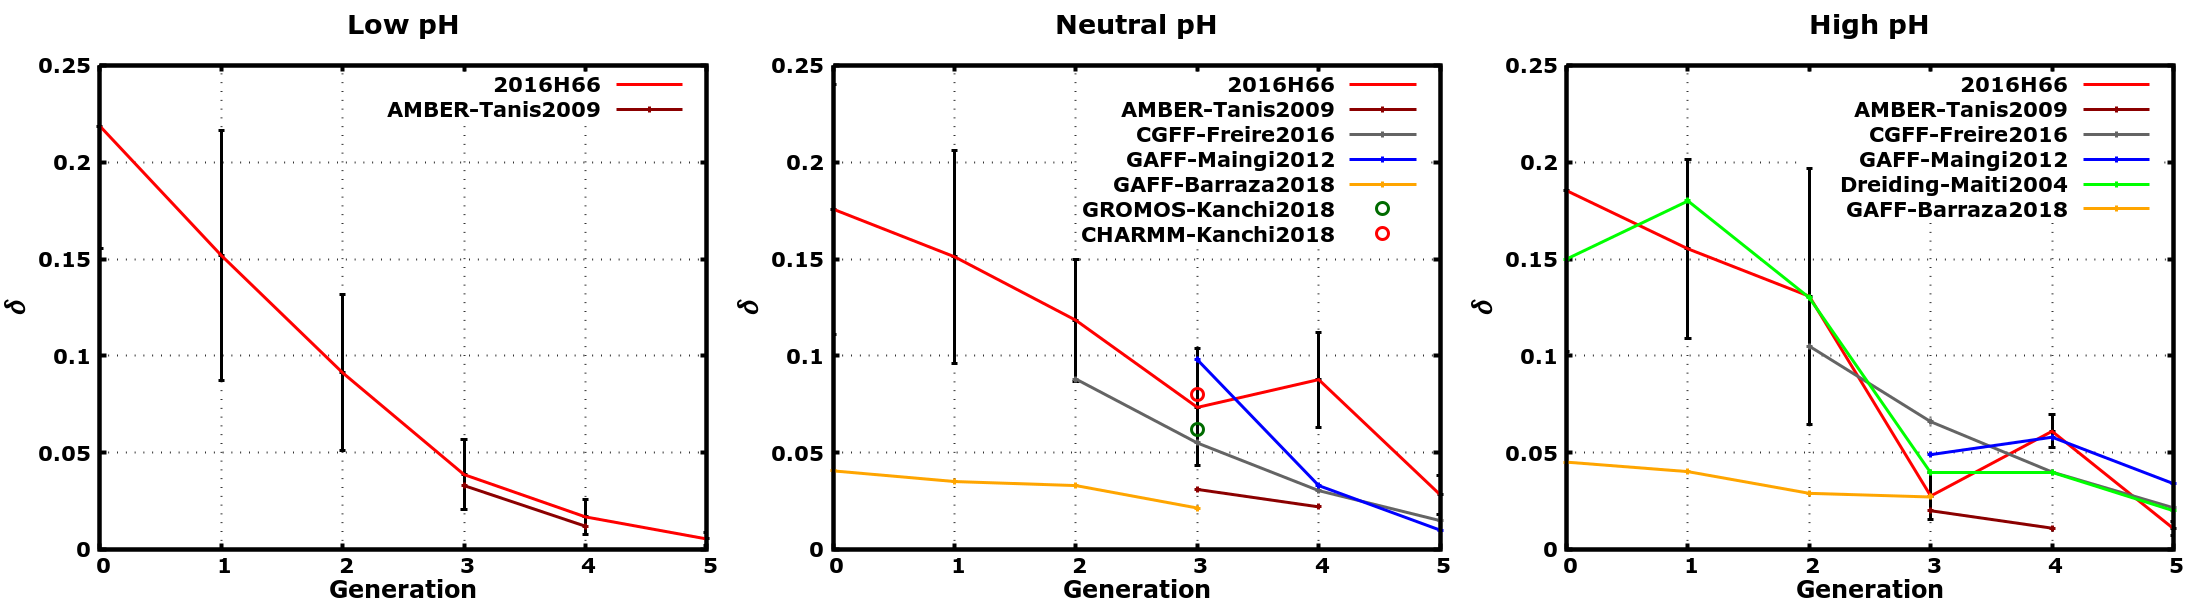
\includegraphics[width=\textwidth]{images/PAMAMAsphericity.png}
\caption{Asfericidade $\delta$ do PAMAM em função da geração. As curvas da esquerda para a direita mostram, respectivamente, os sistemas em baixo, neutro e alto pH.
Os resultados obtidos com o campo de força 2016H66\cite{Horta2016} são comparados com resultados de estudos experimentais e de simulações prévios:
Maiti2004\cite{Maiti2004}, %\cite{MA04.18},
Tanis2009\cite{Tanis2009}, %\cite{TA09.6},
Maingi2012\cite{Maingi2012}, %\cite{MA12.23},
Freire2016\cite{Freire2016}, %\cite{FR16.Y}.}
Barraza2018\cite{Barraza2018}.} %\cite{BA18.Y} and
\label{fig:PAMAMAsphericity}
\end{figure*}

\begin{table*}
\centering
    \begin{tabular}{cccccccc}
 \hline
 $GN$     & pH  & Iz/Iy &   Iz/Ix   & Asphericity\\
 \hline
 \hline 
 G0     &  \multirow{6}{*}{Acid}    &   1.2219& 1.6535& 0.2187\\
 G1     &                           &   1.5497& 1.9441& 0.1518\\
 G2     &                           &   1.1938& 1.6545& 0.0913\\
 G3     &                           &   1.2680& 1.4044& 0.0387\\
 G4     &                           &   1.3583& 1.1048& 0.0168\\
 G5     &                           &   1.0285& 1.0557& 0.0054\\
 \hline 
 G0     &  \multirow{6}{*}{Neutral} &   1.2775& 3.0340& 0.1757\\
 G1     &                           &   1.1420& 2.6886& 0.1511\\
 G2     &                           &   1.1455& 1.8338& 0.1183\\
 G3     &                           &   1.0582(1.69)& 1.1380(3.19)& 0.0734(0.098)\\
 G4     &                           &   1.1020(1.17)& 1.6704(1.93)& 0.0877(0.033)\\
 G5     &                           &   1.1473(1.13)& 1.3964(1.41)& 0.0283(0.010)\\
 \hline 
 G0     &  \multirow{6}{*}{Basic}   &   1.1418& 2.2922& 0.1853\\
 G1     &                           &   1.3091& 2.0219& 0.1552\\
 G2     &                           &   1.0367& 1.4595& 0.1308\\
 G3     &                           &   1.1530(1.38)& 1.3704(2.21)& 0.0276(0.049)\\
 G4     &                           &   1.3277(1.41)& 1.4790(2.44)& 0.0610(0.058)\\
 G5     &                           &   1.0807(1.29)& 1.2036(1.93)& 0.0108(0.034)\\
 \hline
    \end{tabular}
\caption{Tabela com os valores de razão de aspecto e asfericidades calculados com o 2016H66 para o PAMAM.
Os valores entre parênteses são dados retirados do estudo de Maingi \textit{et al}\cite{Maingi2012}.}
\label{tab:PAMAMAsfericidade}
\end{table*}

Em baixo pH, vemos um decaimento monotônico da asfericidade $\delta$ com o aumento da geração tendendo à uma esfera, ou seja, $\delta \sim 0$. 
Tanis e Karatasos\cite{Tanis2009} reportaram praticamente os mesmo valores obtidos por esse trabalho para dendrímeros de geração $3$ e $4$ em baixo pH fazendo uso do campo de força AMBER\cite{Weiner1984} e solvente explícito.

Já em pH neutro, o 2016H66 continua a mostrar um decaimento da asfericidade com a geração, mas um leve aumento ocorre na geração 4.
Valores similares foram encontrados por Maingi \textit{et al}\cite{Maingi2012} com o GAFF, Freire \textit{et al}\cite{Freire2016} com um campo de força \textit{coarse grained} e por Kanchi \textit{et al}\cite{Kanchi2018} tanto com GROMOS quanto com o CHARMM para a terceira geração.
Mas eles não apresentam o aumento mostrado pelo 2016H66\cite{Horta2016} em pH neutro.
Outros estudos como o do Barraza \textit{et al}\cite{Barraza2017} com GAFF e do Tanis e Karatasos\cite{Tanis2009} com o AMBER\cite{Weiner1984} apresentam valores muito menores do que é comumente reportado na literatura.

Quando analisamos o sistema em pH alto, os valores reportados por Maingi \textit{et al}\cite{Maingi2012} e por Maiti \textit{et al}\cite{Maiti2004} apresentam o mesmo comportamento na geração 4 que o 2016H66\cite{Horta2016} com valores numéricos significativamente próximos.
A simulação \textit{coarse grained} de Tanis \textit{et al}\cite{Tanis2009} mostra novamente um decaimento monotônico assim como em pH neutro.
E o comportamento reportado por Barraza \textit{et al}\cite{Barraza2017} e por Tanis e Karatasos\cite{Tanis2009} também continua o mesmo.

Trabalhos teóricos sugerem que a mudança da geração 3 para a 4 é caracterizada por um aumento substancial do \textit{back-folding} nos dendrímeros.
Sendo discutido até mesmo que seu padrão estrutural de \textit{dense core} poderia passar a ser melhor descrito como um \textit{dense shell} dependendo do tamanho do terminal.
Essa mudança, contudo, não ocorre no PAMAM.
Como veremos mais à frente, as curvas de distribuição radial (RDF) revelam, de fato, um aumento na quantidade de \textit{back-folding} nessa passagem.

\subsection{Estrutura}\label{PAMAMEstrutura}

As curvas de função de distribuição radial foram calculadas como descrito na Seção \ref{RDF} e os resultados estão mostrados na Figura \ref{fig:PAMAMRDF}.

\begin{figure*}[ht!]
\centering
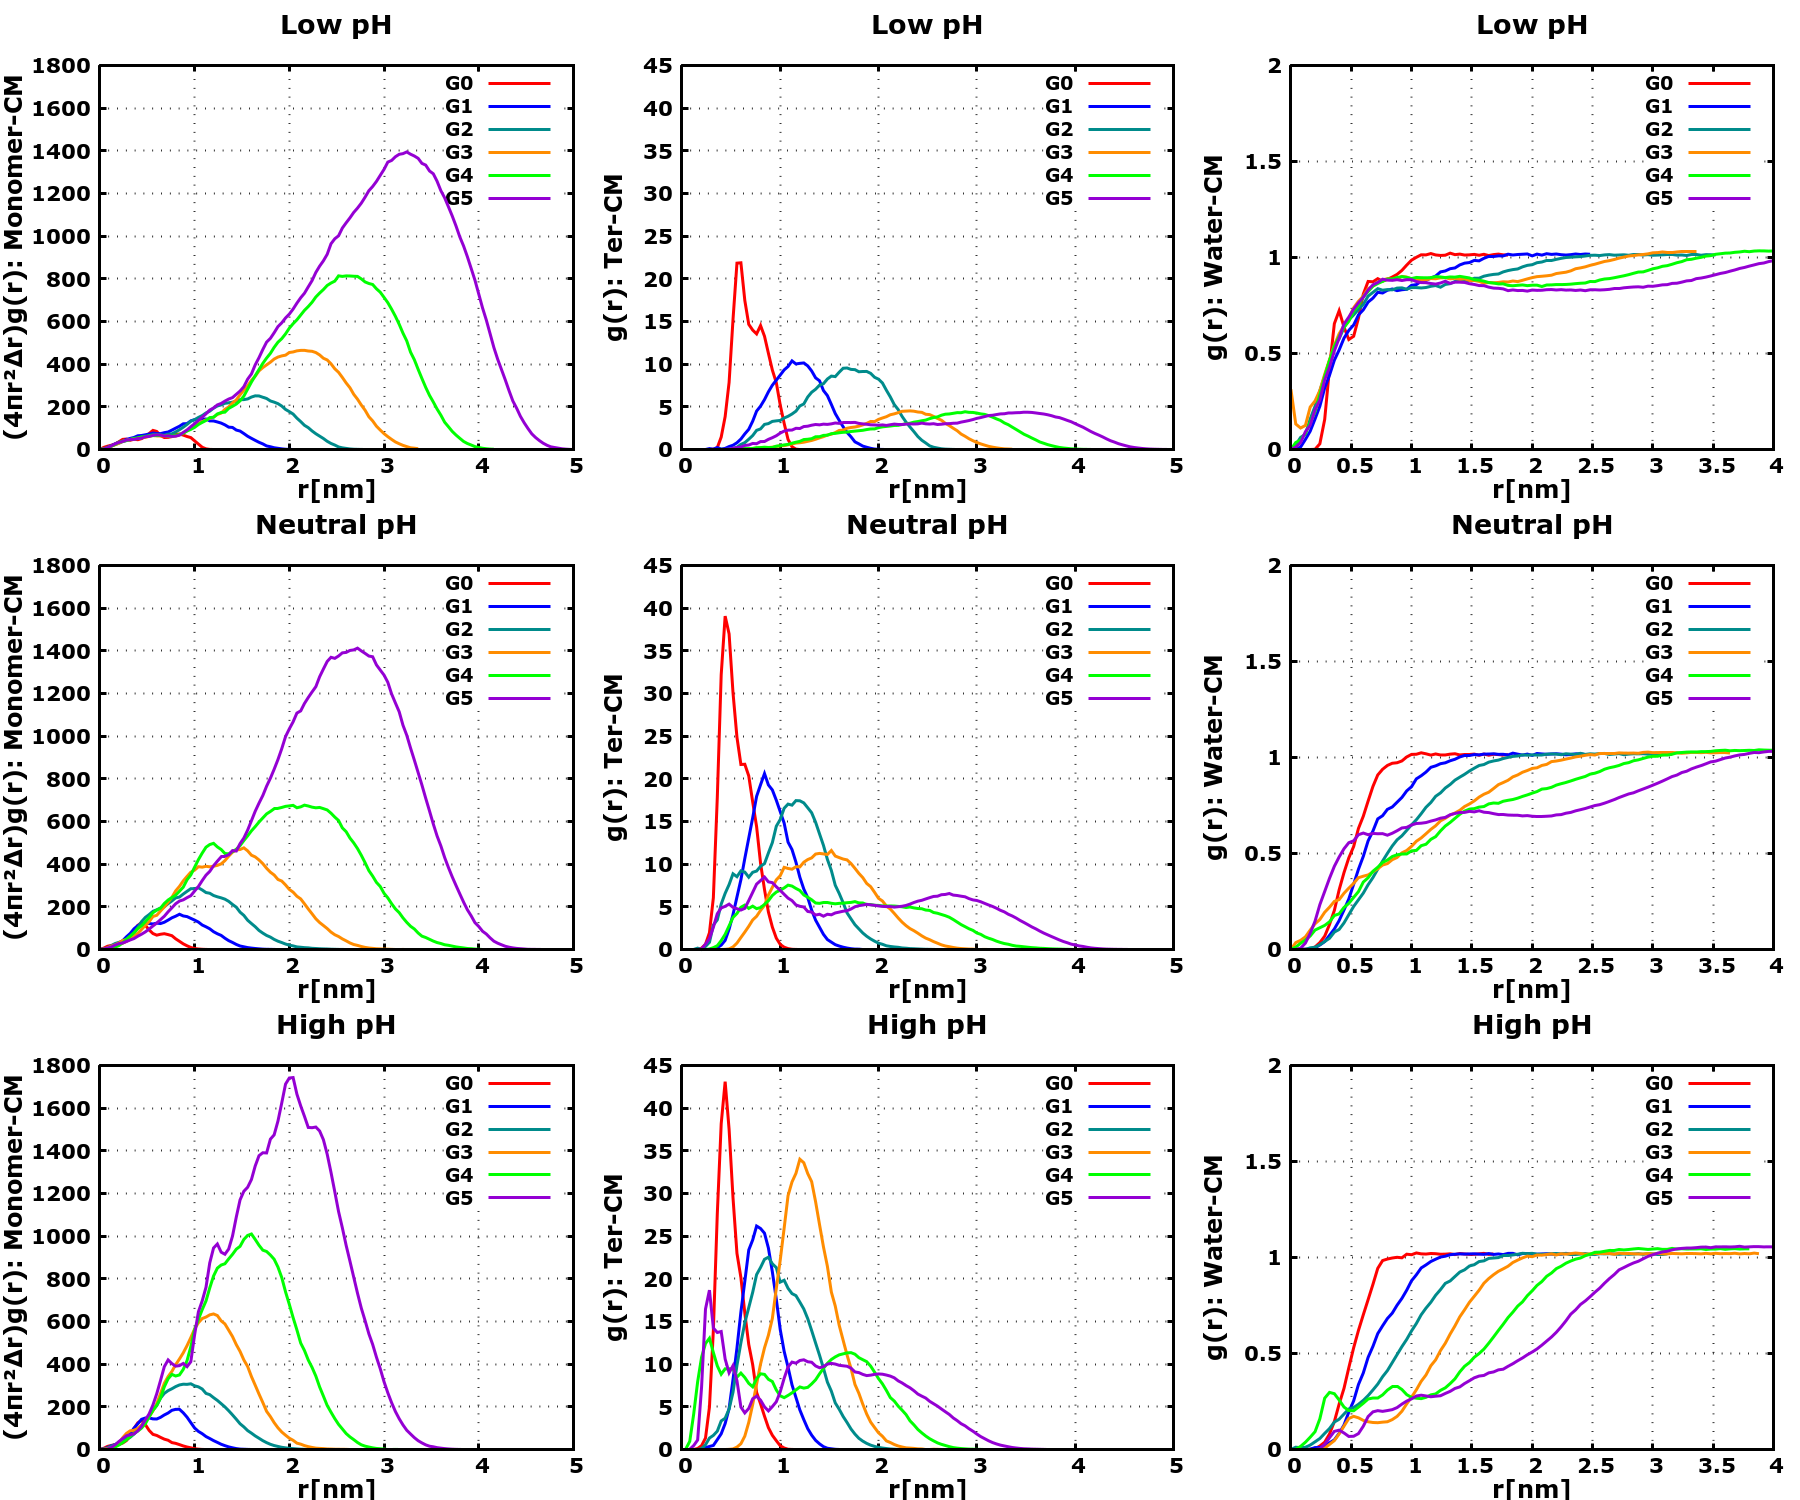
\includegraphics[width=\textwidth]{images/PAMAMRDF.png}
\caption{Função de distribuição radial (RDF) $g(r)$ para o PAMAM. As curvas da esquerda, do meio e da direita mostram, respectivamente, as RDFs do centro de massa do dendrímero em relação à todos os átomos do dendrímero, às aminas primárias terminais e às moléculas de água. E as linhas superiores, intermediárias e inferiores mostram os RDFs descritos anteriormente em condições de pH baixo, neutro e alto, respectivamente. A coluna da esquerda não foi normalizada pelo volume da camada esférica utilizada.}
\label{fig:PAMAMRDF}
\end{figure*}

A curva da esquerda mostra a função de distribuição radial sem efetuar a divisão pelo volume da casca esférica considerada no cálculo. Na prática, é o mesmo que calcular $4\pi r^2 \Delta r \times g(r)$.
Dessa forma, não podemos interpretá-la como um perfil de densidade, mas como um valor proporcional ao número absoluto de átomos contados. 
Ela mostra que o aumento da geração faz com que se forme um acúmulo de átomos na região superfícial do dendrímero.
Esse comportamento é o mesmo obtido por Lee \textit{et al}\cite{Lee2002} que pode ser visto na coluna da esqueda da Figura 11 em seu estudo.
É intuitivo pensar dessa forma devido ao fato de que cada nova geração tem o dobro de aminas terminais que a geração anterior. 
Os autores acreditam que isso foi o motivador principal para caracterizar, errôneamente, dendrímeros pelo modelo de \textit{dense shell} já que essas curvas não podem ser interpretadas como densidades.
Nela, podemos ver, também, o efeito do pH na estrutura dendrítica do PAMAM.
Conforme o pH se torna mais ácido (ou mais baixo), a distribuição se torna mais larga.
Indicando que o tamanho da molécula aumenta e que, devido à concentração de átomos na superfície, ela apresenta cavidades maiores (ou mais espaços vazios).
Isso se deve ao fato de que a protonação das aminas cria uma forte repulsão entre elas. Isso gera um afastamento que possibilita a entrada de solvente na estrutura.
Esse inchaço é amplamente reportado na literatura e foi visto ser capturado pelas simulações com o 2016H66\cite{Horta2016}.
 
A coluna do meio da Figura \ref{fig:PAMAMRDF} apresenta a função de distribuição radial das aminas primárias terminais em relação ao centro de massa do dendrímero.
Essas curvas foram normalizadas pelo volume da casca esférica. 
Por isso, podem ser chamadas de perfil de densidade das aminas terminais. 
Note que essa curva está completamente diferente das curvas reportadas por Lee \textit{et al}\cite{Lee2002} na coluna da direita da Figura 11 em seu trabalho e por Brocorens \textit{et al}\cite{Brocorens2005} na Figura 6 do seu trabalho.
A principal diferença é que ambos estão calculando funções de distribuição, e não perfis de densidade.
Como o que é calculado por Maiti \textit{et al}\cite{Maiti2004} na Figura 7 de seu trabalho e por Bellini \textit{et al}\cite{Bellini2015} na subfigura d) da Figura 2 de seu estudo, as curvas se assemelham substancialmente às reportadas nesse trabalho. 
Novamente podemos ver que para baixos pHs, o tamanho do dendrímero é maior.

Interessantemente, nesses gráficos é possível ver que mesmo com o aumento da geração, a existênciade densidade de aminas terminais ao longo de todo o volume da molécula se mantêm.
Isso se deve à formação de \textit{back-folding}, como discutido anteriormente.

O efeito do pH é de expandir a estrutura devido à repulsão eletrostática gerada pelas aminas protonadas e consequente hidratação da estrutura. Aqui vemos que a maior compactação da estrutura em pH alto é devido ao maior grau de \textit{back-folding} das aminas terminais. 
E mesmo após protonação das aminas (pH baixo) ainda é possível observar a existência de \textit{back-folding} no sistema. 
Como uma pequena massa do sistema está localizada no centro do dendrímero (devido às cavidades internas da estrutura) o fator entrópico de formar o \textit{back-folding} de partes mais externas da estrutura vence a penalidade causada pela interação de volume excludente.
Então, mesmo que energeticamente seja desfavorável, é entropicamente favorável que ocorra \textit{back-folding} em dendrímeros de gerações maiores\cite{Rathgeber2004}.

A coluna da direita mostra a distribuição de densidade radial de moléculas de água ao redor do centro de massa do dendrímero. 
Colaborando para construir as mesmas conclusões obtidas nas outras distribuições, em baixo pH a curva apresenta altos valores bem próximo ao centro do dendrímero, revelando que há uma grande quantidade de moléculas de água ao longo de todo volume da molécula.
Conforme aumentamos o pH, a estrutura vai se tornando mais compacta e a densidade de água no interior do dendrímero vai diminuido.
Esse comportamento é majoritariamente percebido para maiores gerações.
Dendrímeros de menores gerações não têm uma estrutura complexa o suficiente para permitir um alto grau de \textit{back-folding} que evitaria a entrada de água.
Esse resultado se assemelha ao reportado por Wu \textit{et al}\cite{Wu2012} para o PAMAM de geração 4 na Figura 7 de seu estudo.

\begin{figure*}[ht!]
\centering
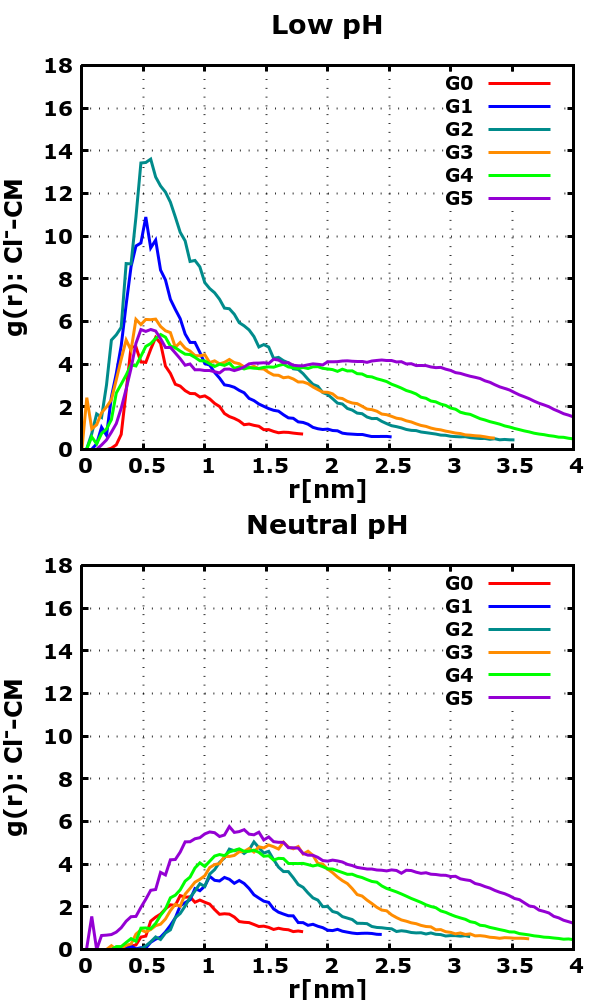
\includegraphics[scale=0.3]{images/PAMAMClRDF.png}
\caption{Função de densidade radial $g(r)$ para o PAMAM. As curvas mostram o RDF de contra-íons Cloreto em relação ao centro de massa do dendrímero para os casos onde o contra-íon está presente(pHs alto e neutro).}
\label{fig:PAMAMClRDF}
\end{figure*}

A Figura \ref{fig:PAMAMClRDF} apresenta os perfis de densidade de íons cloreto no sistema.
É interessante perceber que (imagem de cima da Figura \ref{fig:PAMAMClRDF}), a curva de distribuição dos íons apresenta um pico muito próximo do centro do dendrímero em pH baixo independentemente da geração, devido à maior concentração de carga no interior da molécula nesse pH.
Como a carga no interior da estrutura nesse pH é altamente positiva, os íon são fortemente atraídos para os sítios de carregados positivamente.
Já em pH neutro, a maior concentração de íons se dá majoritáriamente ao longo da superfície do dendrímero, onde há a concentração de cargas positivas (imagem de baixo da Figura \ref{fig:PAMAMClRDF}).

\begin{landscape}
\begin{table}[t] %PPI Rg Suplemmental info tables
\caption{
Comparação do raio de giro $R_g$ (em nm) calculado na presente dissertação para o PPI com valores disponíveis na literatura.
Os resultados estão organizados de acordo com o pH do meio (baixo, neutro e alto), número da geração $GN$ (de G1 à G6) e método utilizado no tratamento das interações de Lennard-Jones (PME: Particle-Mesh Ewald e CUT: \textit{cut-off scheme} com raio de corte de $1.2$ nm).
Como discutido na Seção \ref{ProtonacaoPPI}, somente os valores com a protonação sugerida pelo modelo de Ising\cite{VanDuijvenbode1998, Koper1997} foram considerados.
Os resultados da literatura mostrados foram tirados dos seguintes estudos:
SAXS(Prosa1997)\cite{Prosa1997},
SANS(Scherrenberg1998)\cite{Scherrenberg1998},
SANS(Topp1999)\cite{Topp1999},
COMPASS/OPLS(Wu2010)\cite{Wu2010},
GAFF(Maingi2012)\cite{Maingi2012},
GAFF(Jain2013)\cite{Jain2013}.}
\centering
\scalebox{0.8}{
\begin{tabular}{ccccccccccccc}
\hline
G$N$   & \multirow{2}{*}{pH}   &\multicolumn{2}{c}{This work}  &COMPASS/OPLS\cite{Wu2010}  &   GAFF\cite{Maingi2012}  &GAFF\cite{Jain2013}  &SANS\cite{Topp1999}  &   SAXS\cite{Prosa1997}   & SANS\cite{Scherrenberg1998}\\
PPI   &                       &       PME     &       CUT     &                       &                       &                   &                   &                       &                   \\
% PPI &                       &       PME     &       CUT     &   Wu2010              &   Maingi2012          &   Jain2013        &   Topp1999        &   Prosa1997           & Scherrenberg1998  \\
\hline
G1   &  \multirow{6}{*}{Low}    &   0.51        &   0.51        &-                      &-                      &   -               &   -               &   -                   &   -   \\
G2  &                          &   0.78        &   0.79        &-                      &-                      &   -               &   -               &   -                   &   -   \\
G3     &                          &   1.04        &   1.06        &-                      &-                      &   -               &   -               &   -                   &   -   \\
G4    &                          &   1.34        &   1.35        &-                      &-                      &   -               &   -               &   -                   &   -   \\
G5   &                          &   1.65        &   1.65        & 1.58                  &-                      &   -               &   -               &   -                   &   -   \\
G6  &                          &   1.99        &   2.00        &-                      &-                      &   -               &   -               &   -                   &   -   \\
\hline
G1    & \multirow{6}{*}{Neutral} &   0.51        &   0.51        &-                      &-                      &   -               & -                 &-                      & 0.44  \\
G2   &                          &   0.77        &   0.77        &-                      &-                      &   -               & -                 &-                      & 0.69  \\
G3  &                          &   1.04        &   1.05        &-                      &-                      &   -               & -                 & 1.13                  & 0.93  \\
G4     &                          &   1.34        &   1.32        &-                      &-                      &   -               & 1.24              & 1.33                  & 1.16  \\
G5    &                          &   1.65        &   1.64        & 1.59                  & 1.61                  &   1.577           & 1.56              & 1.43                  & 1.39  \\
G6   &                          &   1.98        &   1.97        &-                      &-                      &   -               &                   &-                      &   -   \\
\hline
G1     & \multirow{6}{*}{High}    &   0.49        &   0.49        &-                      &-                      &   -               &   -               &   -                   &   -   \\
G2    &                          &   0.74        &   0.74        &-                      &-                      &   -               &   -               &   -                   &   -   \\
G3   &                          &   0.95        &   0.94        &-                      &-                      &   -               &   -               &   -                   &   -   \\
G4  &                          &   1.07        &   1.03        &-                      &-                      &   -               &   -               &   -                   &   -   \\
G5     &                          &   1.25        &   1.31        & 1.23                  &   1.31                &   1.273           &   -               &   -                   &   -   \\
G6    &                          &   1.60        &   1.56        &-                      &-                      &   -               &   -               &   -                   &   -   \\
\hline   \end{tabular}}
\label{tab:PPIRgValidacao}
\end{table}
\end{landscape}

\section{PPI}

Os valores de raios de giro calculados estão listados na Tabela \ref{tab:PPIRgValidacao} e foram calculados de acordo com o procedimento descrito na Seção \ref{RaioDeGiro} para os sistemas PPI relatados na Seção \ref{SistemasSimulados} e na Tabela \ref{tab:sistemas}.
Em meio neutro, o grau de protonação considerado nessa discussão é o proposto pelo modelo de Ising\cite{VanDuijvenbode1998, Koper1997} como discutido na Seção \ref{ProtonacaoPPI}.

\subsection{Tamanho}\label{PPITamanho}

\begin{figure*}[ht!]
\centering
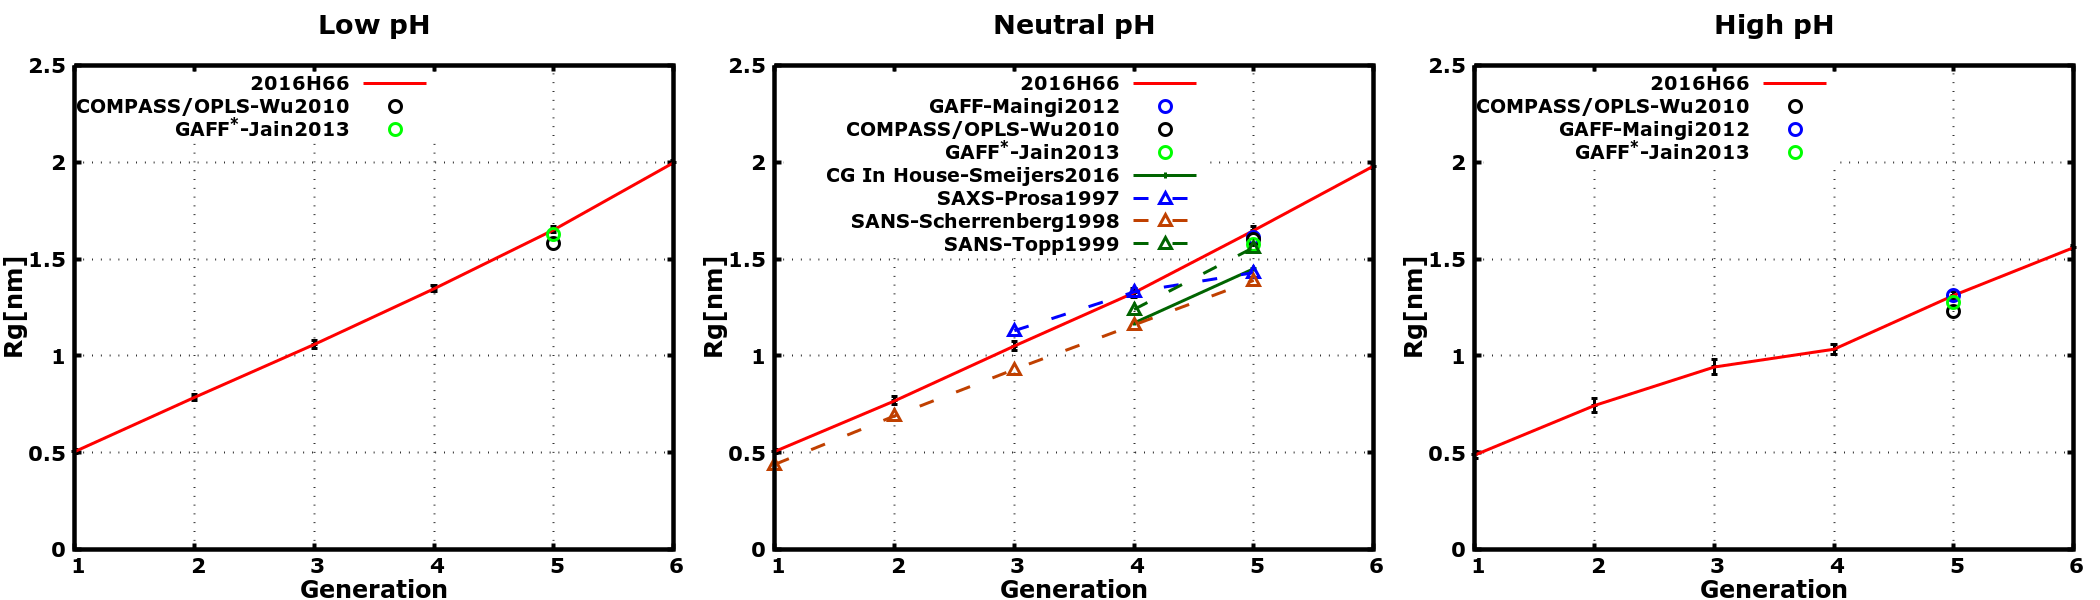
\includegraphics[width=\textwidth]{images/PPIRg.png}
\caption{Raio de giro ($R_g$) em função da geração em meios de pH baixo (curva da esquerda), neutro (curva do meio) e alto (curva da direita).
Os resultados obtidos com o campo de força 2016H66\cite{Horta2016} são comparados com resultados de estudos experimentais e de simulações prévios:
Prosa1997\cite{Prosa1997}, %\cite{PR97.2},
Scherrenberg1998\cite{Scherrenberg1998}, %\cite{SC98.Y},
Topp1999\cite{Topp1999}, %\cite{TO99.Y},
Wu2010\cite{Wu2010}, %\cite{WU10.5},
Maingi2012\cite{Maingi2012}, %\cite{MA12.23},
Jain2013\cite{Jain2013}, %\cite{JA13.4}}
Smeijers2016\cite{Smeijers2016}.} %\cite{SM16.Y}
\label{fig:PPIRg}
\end{figure*}

Um problema encontrado na validação do PPI, é a falta de dados reportados na literatura para tal. Muitos dos estudos efetuados com o PPI são fortemente focados em aplicações.
Por isso, não foram encontrados estudos de simulação sistemáticos onde a influência do raio de giro foi levado em conta.
Principalmente em pHs ácido e básico, onde não haviam dados experimentais disponíveis.

Em baixo pH, na Figura \ref{fig:PPIRg}, os resultados do 2016H66\cite{Horta2016} está em excelente acordo com os trabalhos de Wu\cite{Wu2010}, que utiliza um campo de força composto por uma mistura de parâmetros do Compass\cite{Sun1998} e do OPLS-AA\cite{Jorgensen1996}, e de Jain \textit{et al}\cite{Jain2013} que aplica o GAFF\cite{Wang2004} em um PPI com núcleo de EDA, ao inves de DAB como feito nesse trabalho.
Contudo, os resultados são bem próximos mostrando que um núcleo diferente mas com mesma valência não influencia fortemente o raio de giro da molécula.

Já em pH neutro, há uma maior quantidade de dados, inclusive experimentais, para comparação.
Nesse meio, os resultados para a geração 5 de Wu\cite{Wu2010} e de Jain \textit{et al}\cite{Jain2013} continuam a ter um excelente acordo com o 2016H66\cite{Horta2016}. 
Os resultados obtidos com o 2016H66\cite{Horta2016} também estão em bom acordo com o estudo de Maingi \textit{et al}\cite{Maingi2012}.
Para a mesma geração, dados de SANS reportados por Topp \textit{et al}\cite{Topp1999} mostram relativo acordo com os trabalhos de simulação apresentados.
Esse trabalho com SANS mostra um raio de giro em torno de $0.1$ nm menor que o obtido pelo 2016H66\cite{Horta2016}.
Essa diferença se mantém quando em geração 4.
Outro conjunto de valores reportados por SANS estão disponíveis no estudo de Scherrenberg \textit{et al}\cite{Scherrenberg1998}.
Considerando esse conjunto, os resultados obtidos com o 2016H66\cite{Horta2016} continuam a consistentemente superestimar os dados experimentais, mas não mais com uma diferença constante.
Pode-se ver que a divergência entre os dados aumenta com o aumento da geração do PPI.
Curiosamente, os dados de SAXS reportados por Prosa \textit{et al}\cite{Prosa1997} novamente apresentam um perfil fortemente discordante do padrão aproximadamente linear visto nos outros conjuntos apresentados, assim como para seu estudo no PAMAM.
%%%%%%%%%%%%%%%%%%% SANS BRUNO %%%%%%%%%%%%%%%%%%%
Mesmo com todos os problemas reportados anteriormente para dados de SANS\cite{Porcar2008} na Seção \ref{PAMAMTamanho} (principalmente a invariância com o pH) que sugeriam que estudos de SAXS\cite{Rathgeber2002} seriam mais indicados para o estudo de dendrímeros, o cenário para o PPI ainda é inconclusivo.
Nada pode ser afirmado uma vez que não existem dados de estudos experimentais em diferentes pHs para o PPI.

Em pH básico (ou alto), temos o mesmo cenário que em ácido.
Os valores disponíveis por simulação utilizando tanto COMPASS/OPLS-AA\cite{Wu2010} quanto GAFF com núcleos de EDA\cite{Jain2013} ou de DAB\cite{Maingi2012} estão de acordo ao menos para a geração 5.

\begin{figure*}[ht!]
\centering
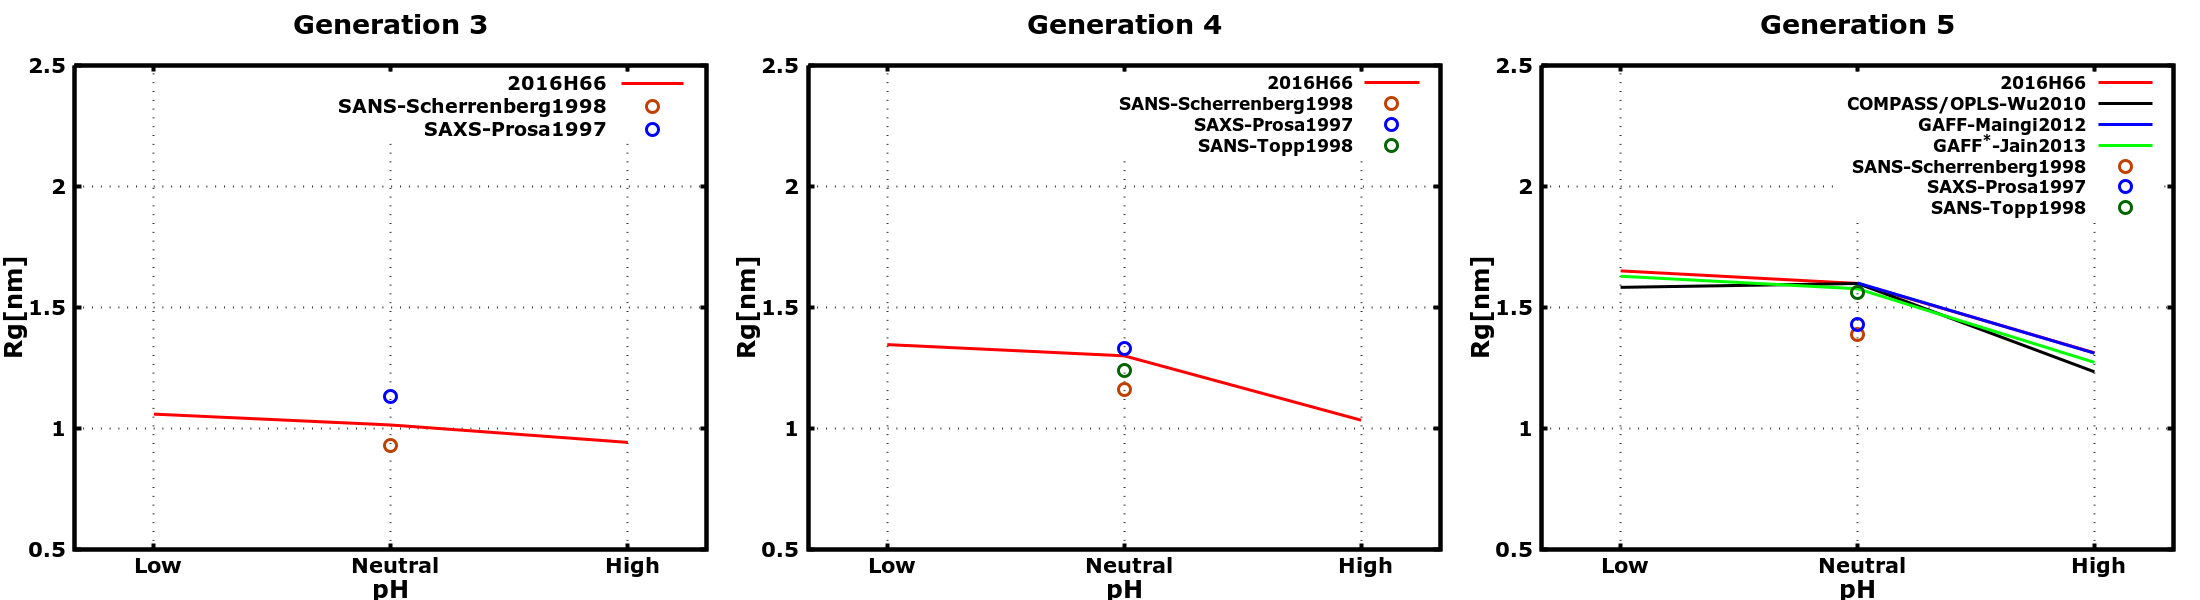
\includegraphics[width=\textwidth]{images/PPIgyrateGpH.png}
\caption{Raio de giro ($R_g$) em função do pH para o PPI de geração 3 (curva da esquerda), 4 (curva do meio) e 5 (curva da direita).
Os resultados obtidos com o campo de força 2016H66\cite{Horta2016} são comparados com resultados de estudos experimentais e de simulações prévios:
Prosa1997\cite{Prosa1997}, %\cite{PR97.2},
Scherrenberg1998\cite{Scherrenberg1998}, %\cite{SC98.Y},
Topp1999\cite{Topp1999}, %\cite{TO99.Y},
Wu2010\cite{Wu2010}, %\cite{WU10.5},
Maingi2012\cite{Maingi2012}, %\cite{MA12.23},
Jain2013\cite{Jain2013}, %\cite{JA13.4}}
Smeijers2016\cite{Smeijers2016}.} %\cite{SM16.Y} and
\label{fig:PPIRgpH}
\end{figure*}

Na Figura \ref{fig:PPIRgpH}, mostramos a mesma análise feita para o PAMAM na Figura \ref{fig:PAMAMRgpH}.
Nela podemos ver com mais detalhes principalmente o sistema em pH neutro, já que em pH ácido e básico os trabalhos de simulação estão em excelente acordo com o 2016H66\cite{Horta2016}.
Vale notar que os pontos em geração 5 (imagem da direita na Figura \ref{fig:PPIRgpH}) para o 2016H66\cite{Horta2016} e para GAFF\cite{Mayo1990} reportados por Maingi \textit{et al}\cite{Maingi2012} se sobrepõem.
Consultando a Tabela \ref{tab:PPIRgValidacao}, vemos que em pH neutro o 2016H66\cite{Horta2016} e o GAFF\cite{Maingi2012} resultam em $1.599$ nm e $1.601$ nm e, em pH alto, $1.312$ nm e $1.311$ nm, respectivamente.

É interessante notar que praticamente todo inchaço visto no PPI acontece quando as aminas primárias (terminais) são protonadas.
A protonação das aminas terciárias (intermediárias) causa um efeito muito menor no raio de giro da molécula.
A Figura \ref{fig:PPIRgpH} e o Tabela \ref{tab:PPIRgValidacao} mostra que, para a geração 4, na passagem do pH alto para o neutro, ou seja, quando as aminas terminais são protonadas, o raio de giro vai de $1.03$ nm para $1.32$ nm.
Um inchaço relativo de, aproximadamente, $22\%$.
Enquanto quando varia o pH de neutro para baixo, têm-se um inchaço de apenas 2\%, mesmo que as aminas terciárias estejam numa região mais interna do dendrímero. O raio de giro em pH baixo é de $1.35$ nm.


\subsection{Forma}\label{PPIForma}

Os fatores de forma e asfericidades foram calculados de acordo com o descrito na Seção \ref{Asfericidade} para os sistemas reportados na Seção \ref{SistemasSimulados}.
Os valores das propriedades obtidas estão disponíveis na Tabela \ref{tab:PPIAsfericidade}.
Sob as suposições discutidas na Seção \ref{EfeitoDoSetup}, somente as propriedades obtidas com o esquema de avaliação das interações de Lennard-Jones sendo o \textit{cut-off} e considerando o estado de protonação proposto pelo modelo de Ising\cite{VanDuijvenbode1998, Koper1997} para o pH neutro são exibidos.

\begin{figure*}[ht!]
\centering
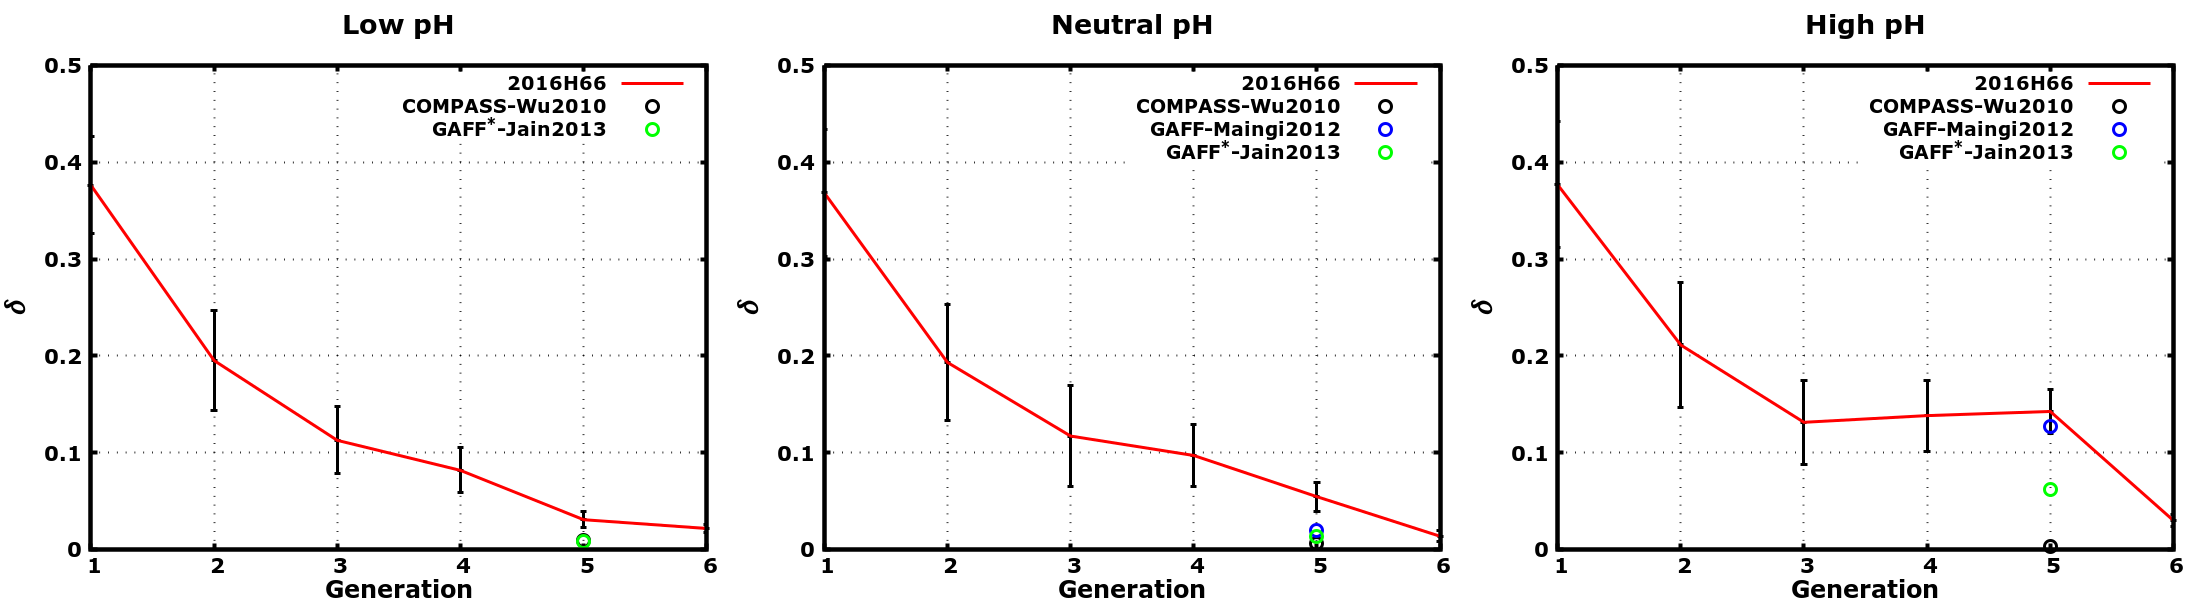
\includegraphics[width=\textwidth]{images/PPIAsphericity.png}
\caption{Asfericidade $\delta$ do PPI em função da geração. As curvas da esqueda para a direita mostram os sistemas em baixo, neutro e alto pH, respectivamente.
Os resultados obtidos com o campo de força 2016H66\cite{Horta2016} são comparados com resultados de estudos experimentais e de simulações prévios:
Wu2010\cite{Wu2010}, %\cite{WU10.5}, 
Maingi2012\cite{Maingi2012}, %\cite{MA12.23}, 
Jain2013\cite{Jain2013}.} %\cite{JA13.4}}
\label{fig:PPIAsphericity}
\end{figure*}

\begin{table*}[ht!] %The moments of inertia were calculated, but I don't know if they are really expressives
\centering
    \begin{tabular}{ccccccccccc}
 \hline
 $GN$   & pH  &   Iz/Iy   &   Iz/Ix   & Asphericity   \\
 \hline
 \hline%WU10.Y
 G1     &  \multirow{6}{*}{Acid}    &   1.2555&4.3832&0.3762\\
 G2     &                           &   1.4106&2.2934&0.1951\\
 G3     &                           &   1.3554&1.8071&0.1127\\
 G4     &                           &   1.2671&1.5132&0.0817\\
 G5     &                           &   1.1565&1.3290&0.0308\\
 G6     &                           &   1.1865&1.2995&0.0217\\
 \hline
 G1     &  \multirow{6}{*}{Neutral} &   1.2882&2.8412&0.3685\\
 G2     &                           &   1.3852&2.1706&0.1932\\
 G3     &                           &   1.0299&1.7626&0.1172\\
 G4     &                           &   1.0965&1.7413&0.0971\\
 G5     &                           &   1.1552(1.35)&1.3358(1.58)&0.0546(0.020)\\
 G6     &                           &   1.0670&1.2045&0.0136\\
 \hline
 G1     &  \multirow{6}{*}{Basic}   &   1.2443&3.8218&0.3768\\
 G2     &                           &   1.1224&2.7673&0.2112\\
 G3     &                           &   1.2986&2.3075&0.1314\\
 G4     &                           &   1.1288&2.0480&0.1383\\
 G5     &                           &   1.2782(1.56)&2.0844(4.36)&0.1426(0.127)\\
 G6     &                           &   1.2657&1.3948&0.0299\\
 \hline
    \end{tabular}
\caption{Tabela com os valores de razão de aspecto e asfericidade calculados com o 2016H66 para o PPI. Os valores entre parênteses são dados retirados do estudo de Maingi \textit{et al} \cite{Maingi2012}.}
\label{tab:PPIAsfericidade}
\end{table*}

Como a asfericidade não é uma propriedade quantitativamente mensurável a partir de técnicas experimentais, a escassez de trabalhos disponíveis na literatura dificultou a validação ainda mais nessa etapa.

Em pH baixo, os valores de asfericidade reportados na literatura por Wu \textit{et al}\cite{Wu2012} quanto por Jain \textit{et al}\cite{Jain2013} estão em acordo com os resultados do 2016H66\cite{Horta2016}.

Porém, em pH neutro é possível notar uma distanciação considerável entre os modelos.
Tanto para os citados anteriormente quanto para os dados de Maingi \textit{et al}\cite{Maingi2012}, onde o 2016H66\cite{Horta2016} apresenta um acordo um pouco melhor com esse último.

No pH alto, os resultados de outros estudos de simulação divergem fortemente.
Os resultados de COMPASS/OPLS-AA de Wu \textit{et al}\cite{Wu2010} seguem com uma estrutura fortemente esférica (assim como em outros pHs) enquanto os de Jain \textit{et al}\cite{Jain2013} se tornam menos esféricos, como o esperado.
Dentre os trabalhos disponíveis, o 2016H66\cite{Horta2016} tem um melhor acordo com os dados apresentados por Maingi \textit{et al}\cite{Maingi2012} utilizando o campo de força GAFF\cite{Wang2004}.


\subsection{Estrutura}\label{PPIEstrutura}

\begin{figure}[ht!]
\centering
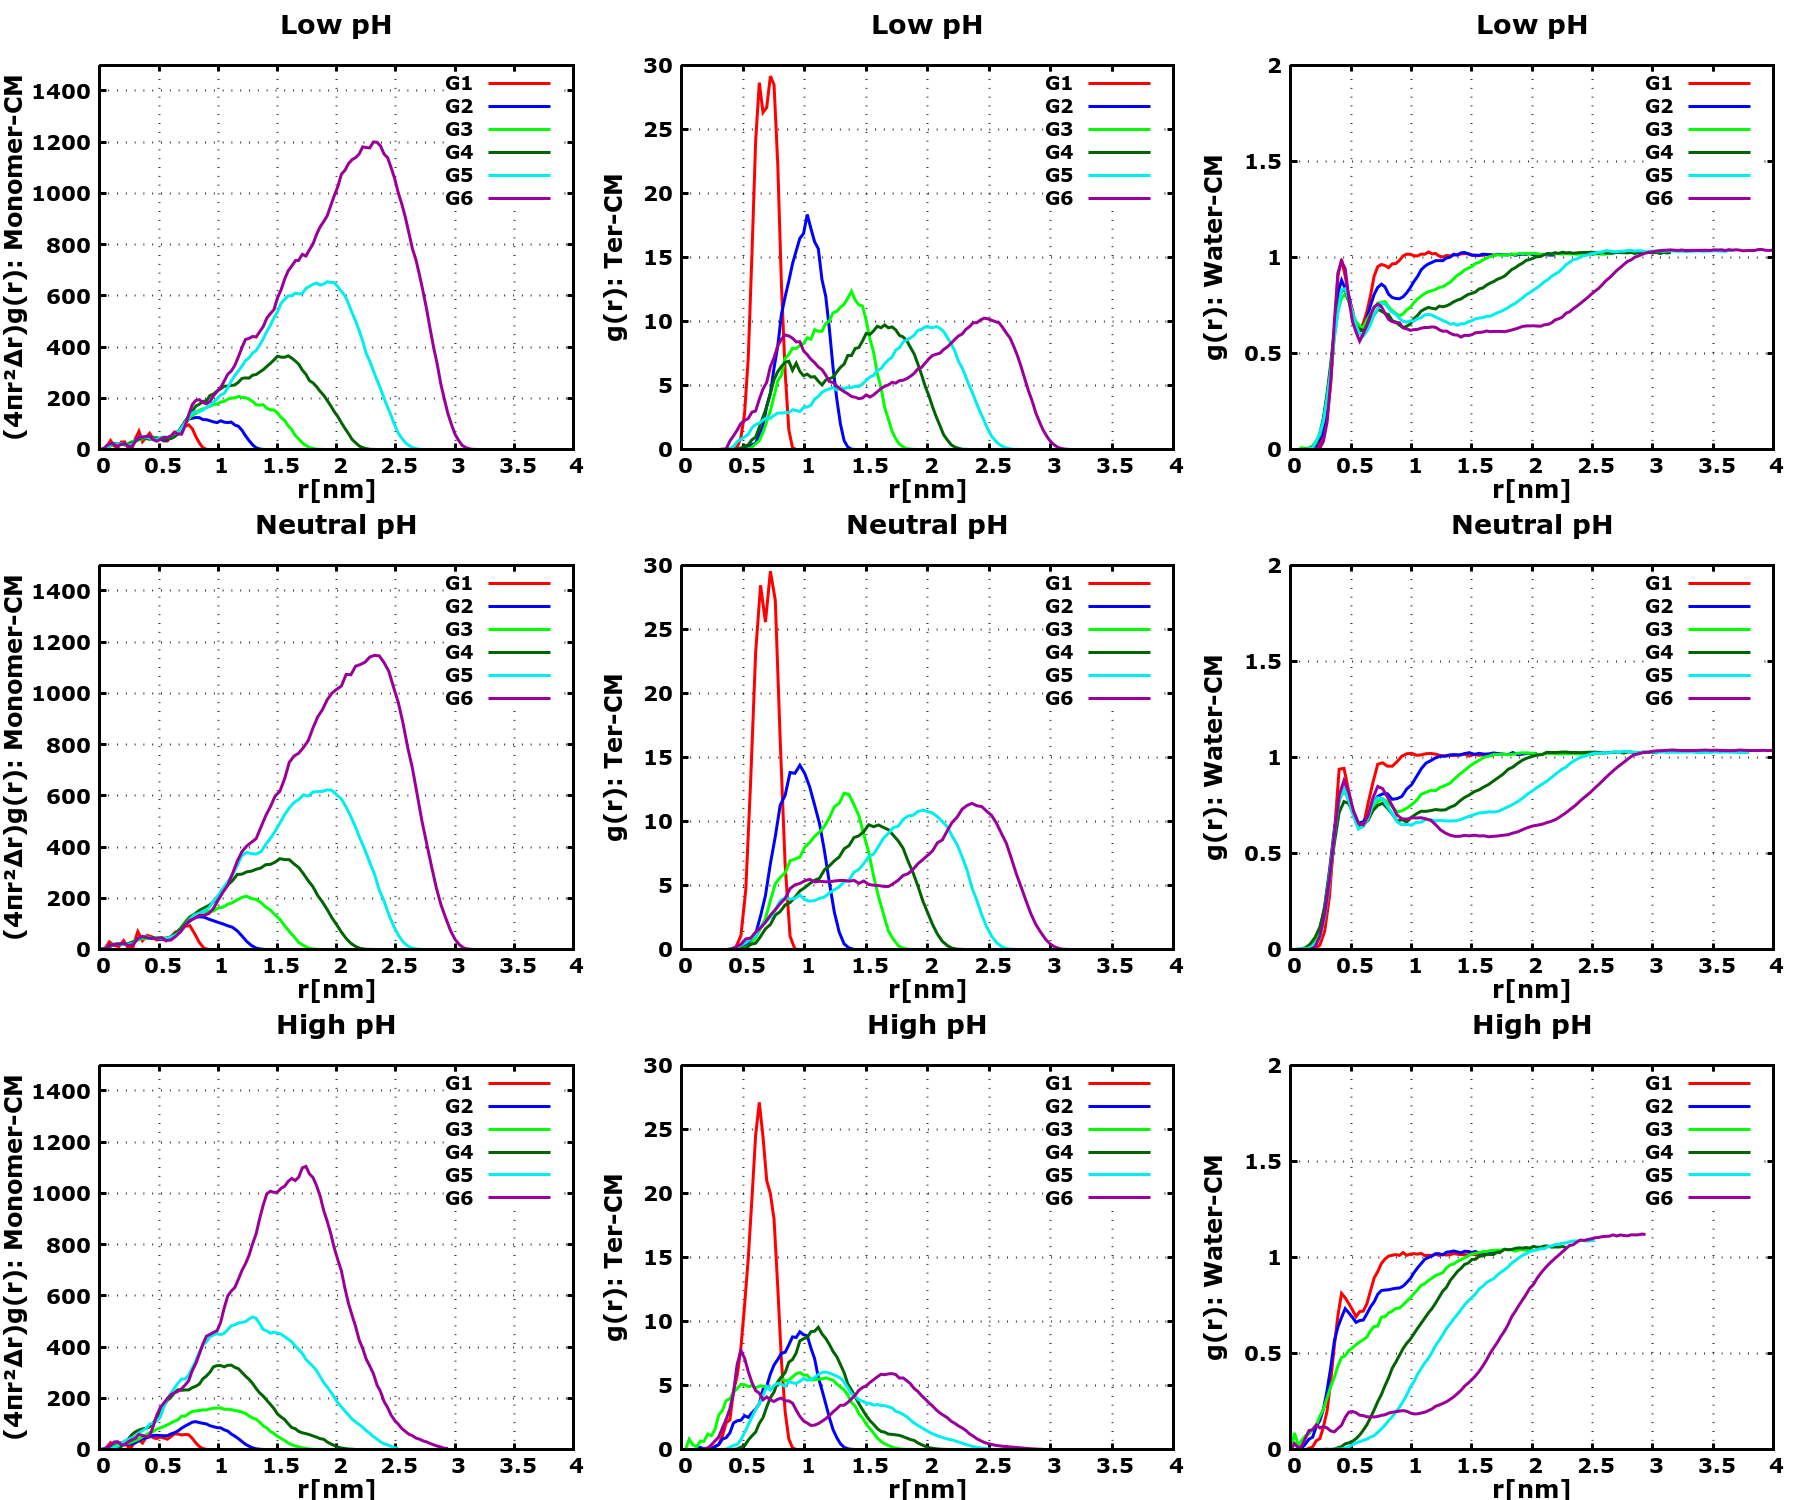
\includegraphics[width=\textwidth]{images/PPIRDF.png}
\caption{Função de distribuição radial (RDF) $g(r)$ para o PAMAM. As curvas da esquerda, do meio e da direita mostram, respectivamente, as RDFs do centro de massa do dendrímero em relação à todos os átomos do dendrímero, às aminas primárias terminais e às moléculas de água. E as linhas superiores, intermediárias e inferiores mostram os RDFs descritos anteriormente em condições de pH baixo, neutro e alto, respectivamente. A coluna da esquerda não foi normalizada pelo volume da camada esférica utilizada.}
\label{fig:PPIRDF}
\end{figure}

A função de distribuição radial foi calculada como descrito na Seção \ref{RDF} e os resultados estão exibidos na Figura \ref{fig:PPIRDF}.
As curvas refletem, no geral, um comportamento bastante parecidos com os do PAMAM.

Na coluna da esquerda, as curvas de distribuição radial de átomos ao redor do centro de massa do dendrímero (sem normalização pelo volume da camada esférica) mostram o inchaço do dendrímero com o abaixamento do pH.
Contudo, esse inchaço é menos abrupto que o observado anteriormente para o PAMAM na Seção \ref{PAMAMEstrutura}.
Os blocos de construção utilizados na montagem do PPI são significativamente menores que os componentes do PAMAM. 
Dessa forma, o incremento de tamanho no PPI com o aumento da geração é bem menor comparado ao PAMAM.
O que podemos perceber pela comparação entre os raios de giro de gerações análogas.
Além disso, de forma geral, o efeito repulsivo e posterior entrada de solvente causada pela protonação de aminas internas no PPI é menos intenso que no PAMAM.

A coluna do meio mostra a densidade radial de aminas terminais em relação ao centro de massa da molécula.
O padrão de alto grau de \textit{back-folding} em alto pH e um menor grau em baixo pH se mantém para o PPI.
Porém, diferentemente do PAMAM, para essa molécula um máximo mais acentuado de densidade de aminas terminais se mantém mais próximo ao centro do dendrímero em pH ácido.
%Como o PPI é um dendrímero menor que o PAMAM, ele apresenta uma menor complexidade em sua estrutura. o que torna possível que as aminas primárias acessem com maior facilidade seu interior.
Mesmo após a protonação da molécula.

A coluna da direita mostra a densidade radial de água no interior da estrutura do dendrímero.
Diferentemente do PAMAM, vemos que em pH neutro, o acesso de solvente no interior da estrutura é maior no PPI.
%Isso se deve à menor complexidade molecular que facilita a difusão de moléculas de água para seu interior.
%Devido à isso, a hidratação em meio neutro e ácido são bastante semelhantes.
Mas em pH básico, o alto grau de \textit{back-folding} continua a ser o efeito dominante, fazendo com que a estrutura mais compacta inviabilise a entrada de solvente.
Este resultado foi reportado, também, por Wu \textit{et al}\cite{Wu2010} na subfigura c da Figura 5 de seu artigo.

As curvas de densidade radiais de cloretos ao redor do centro de massa do dendrímero para o PPI, não difere muito para a do PAMAM. Como pode ser visto na Figura \ref{fig:PPIClRDF}.

\begin{figure}[ht!]
\centering
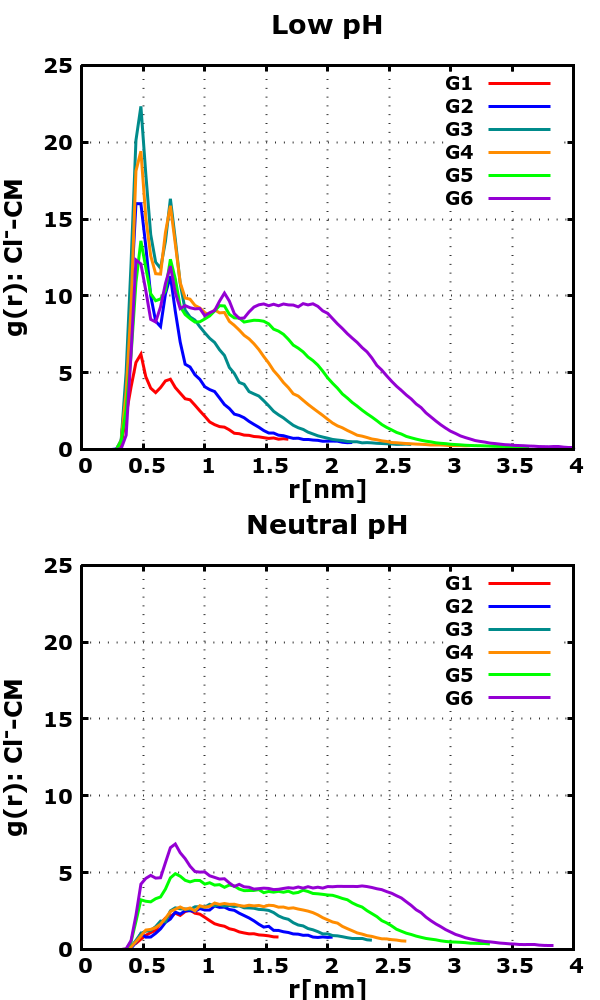
\includegraphics[scale=0.3]{images/PPIClRDF.png}
\caption{Função de distribuição radial g(r) para o PPI. As curvas mostram o RDF de contra-íons cloreto em relação ao centro de massa do dendrímero para os casos onde o contra-íon está presente(pHs alto e neutro).}
\label{fig:PPIClRDF}
\end{figure}

%Como foi discutido anteriormente nessa seção, a difusão de moléculas para o interior do PPI é mais fácil que no PAMAM devido à sua menor complexidade estrutural. 
%Contudo, isso não causa um grande impacto na distribuição de contra-íons.
%A similaridade entre as curvas de distribuições sugere que como átomos de Cloreto são bem menores que moléculas de água, a sua difusão para o interior das estruturas é mais fácil.

\pagebreak


\chapter{Conclusão}

Simulações de dinâmica molecular foram efetuadas para os dendrímeros PAMAM e PPI de geração $1$ à $5$ e $1$ à $6$, respectivamente, utilizando o campo de força \textit{GROMOS-compatible} 2016H66.
As topologias e configurações iniciais das moléculas dendríticas foram criadas com o PyPolyBuilder de maneira automatizada, sendo necessário o mínimo de esforço.
O pacote de simulação Gromacs-5.1.4 foi utilizado seguindo as sugestões de \textit{setup} de Gonçalvez \textit{et al}, mas alterações do método de avaliação das interações de Lennard-Jones não se mostraram de grande impacto no sistema.
Para o PPI, diferentes taxas de protonação foram consideradas para o pH neutro e foi observado que os resultados dessa mudança são bem sutís.
Mas o modelo considerado mais correto pela literatura foi o utilizado nas argumentações da presente dissertação.
As propriedades raio de giro $R_g$, razões de aspecto, asphericidade $\delta$ e funções de distribuição radial foram calculadas e exaustivamente comparadas a dados experimentais, teóricos e computacionais relatados na literatura.
Foi visto que os dados quantitativos de raio de giro $R_g$ calculados pelo 2016H66 se mostraram muitas vezes mais adequados aos resultados experimentais.
Também foi mostrado que os valores relatados de SANS na literatura têm resultados questionáveis e que novos estudos de SAXS e SANS levando em conta o efeito do pH devem ser efetuados para sanar a dúvida em relação ao inchaço dos dendrímeros com alterações no pH ser um artefato das simulações ou modelos ajustados equivocadamente aos dados experimentais.
Por ter melhor se adequado quantitativamente aos experimentos e qualitativamente às predições teóricas, acreditamos que o 2016H66 é um bom campo de força e, ao menos para o cálculo de propriedades estruturais, está devidamente validado para a simulação de dendrímeros e deve ser utilizado em trabalhos futuros nessa linha de pesquisa.

\chapter{Perspectivas futuras}

Tendo sido o campo de forças GROMOS-compatible 2016H66\cite{Horta2016} validado para propriedades estruturais, estudos específicos podem ser iniciados.
Primeiramente a complexação de dendrímeros com fármacos de interesse deve ser estudado para que a validação completa, ou seja, também em propriedades energéticas possa ser conferida.
Após isso, como sugerido anteriormente, os dendrímeros são candidatos promissores como carreadores de fármacos.
Nessa linha de pensamento, novas simulações devem ser efetuadas para o estudo e entendimento desses sistemas.
Futuramente, esse projeto pode seguir as seguintes idéias:
$(i)$   Efetuar simulações de dinâmica molecular dos dendrímeros complexado com moléculas orgânicas de diferentes grupos funcionais e tamanhos de cadeia e avaliar a energia livre de complexação e carregamento máximo. Esse estudo visa obter o entendimento sistemático sobre quais grupos funcionais interagem melhor com o dendrímero e qual o efeito do tamanho de cadeia e do pH do meio nessa complexação;
$(ii)$  Devido à alta toxicidade, provavelmente o dendrímero não poderá ser utilizado $in \; vivo$ na sua forma não-funcionalizada. Por isso, também é interessante o estudo da complexação de fármacos com dendrímeros PEGylados. Espera-se, nesse estudo, entender os efeitos da PEGylação na dinâmica de liberação de fármacos;
$(iii)$ Também, como reportado, o campo de força GROMOS foi o único capaz de reproduzir o resultado experimental em que o dendrímero têm uma adsorção espontânea em membranas lipídicas. Dessa forma, é interessante fazer uso desse campo de força para avaliar a adsorção na membrana e a energia livre associada à permeação do dendrímero pela mesma.

\pagebreak


% ----------------------------------------------------------
% ELEMENTOS PÓS-TEXTUAIS
% ----------------------------------------------------------
\postextual

% ----------------------------------------------------------
% Referências bibliográficas
% ----------------------------------------------------------
\makeatletter
\renewcommand\@biblabel[1]{#1. }
\makeatother

%\bibliographystyle{biblatex-abnt}
\bibliographystyle{abntex2-num}
\bibliography{bibtex.bib}

% ----------------------------------------------------------
% Apêndices
% ----------------------------------------------------------

\begin{apendicesenv}

% Imprime uma página indicando o início dos apêndices
\partapendices

% ----------------------------------------------------------
\chapter{PAMAM utilizando o setup PME} \label{PAMAMap}

\begin{figure}[ht!]
\centering
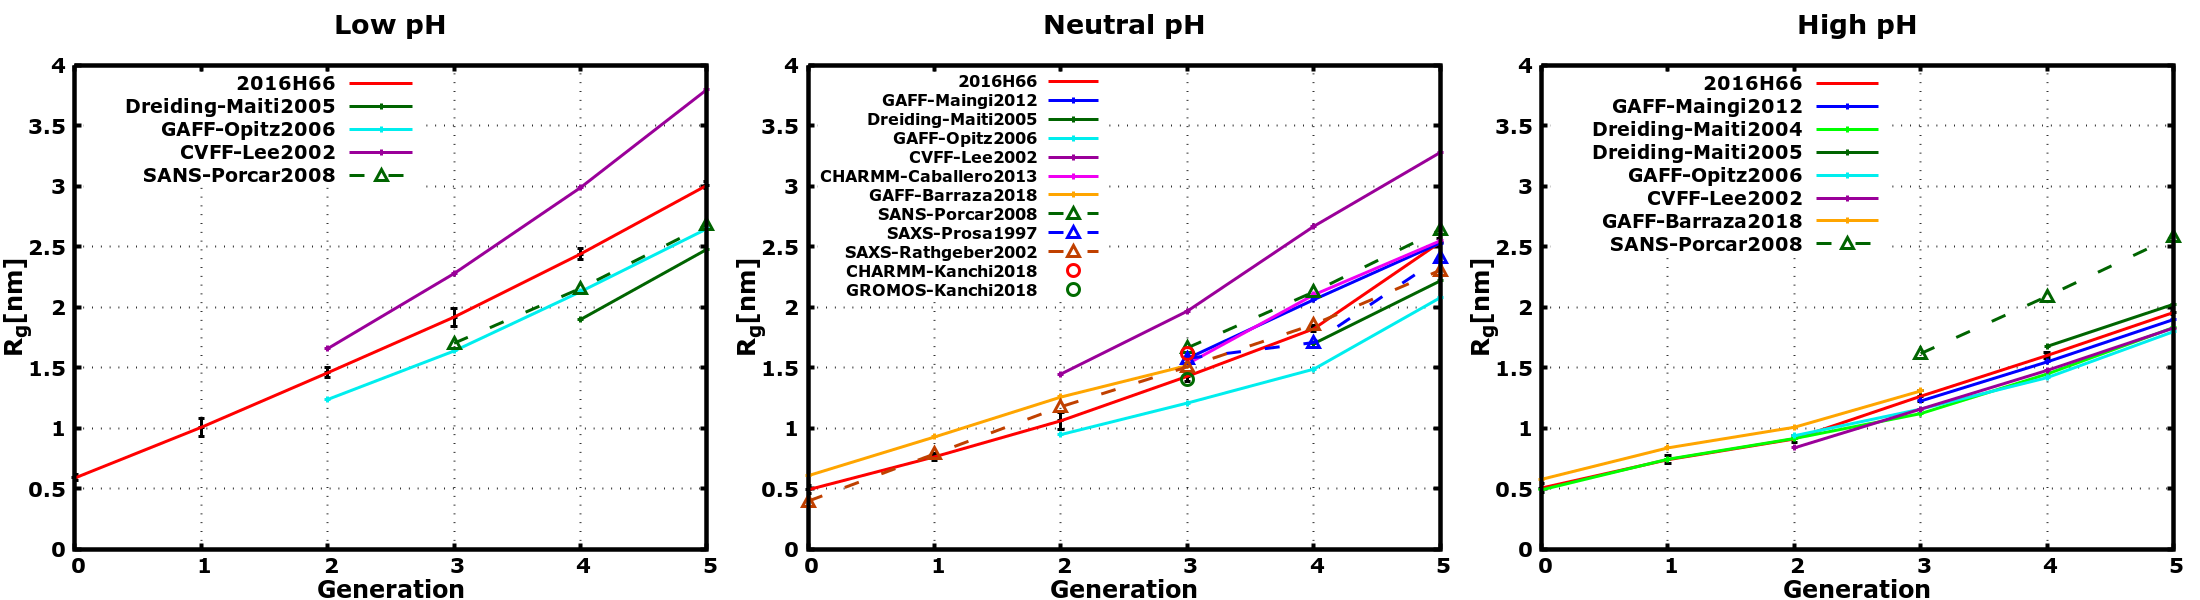
\includegraphics[width=\textwidth]{images/PME/PAMAMRg.png}
\caption{Raio de giro ($R_g$) em função da geração em meios de pH baixo (imagem da esquerda), neutro (imagem do meio) e alto (imagem da direita).
Os resultados obtidos com o campo de força 2016H66\cite{Horta2016} são comparados com resultados de estudos experimentais e de simulações prévios:
Prosa1997\cite{Prosa1997}, %\cite{PR97.2},
Lee2002\cite{Lee2002}, %\cite{LE02.8},
Caballero2013\cite{Caballero2013}, %\cite{CA13.4},
Rathgeber2002\cite{Rathgeber2002}, %\cite{RA02.6},
Maiti2005\cite{Maiti2005}, %\cite{MA05.26},
Opitz2006\cite{Opitz2006}, %\cite{OP06.1},
Porcar2008\cite{Porcar2008}, %\cite{PO08.3},
Maiti2009\cite{Maiti2009}, %\cite{MA09.18},
Maingi2012\cite{Maingi2012}, %\cite{MA12.23},
Barraza2018\cite{Barraza2018}, %\cite{BA18.Y},
Kanchi2018\cite{Kanchi2018}.} %\cite{KA18.Y}.}
\label{supfig:PAMAMRg}
\end{figure}

\begin{figure}[ht!]
\centering
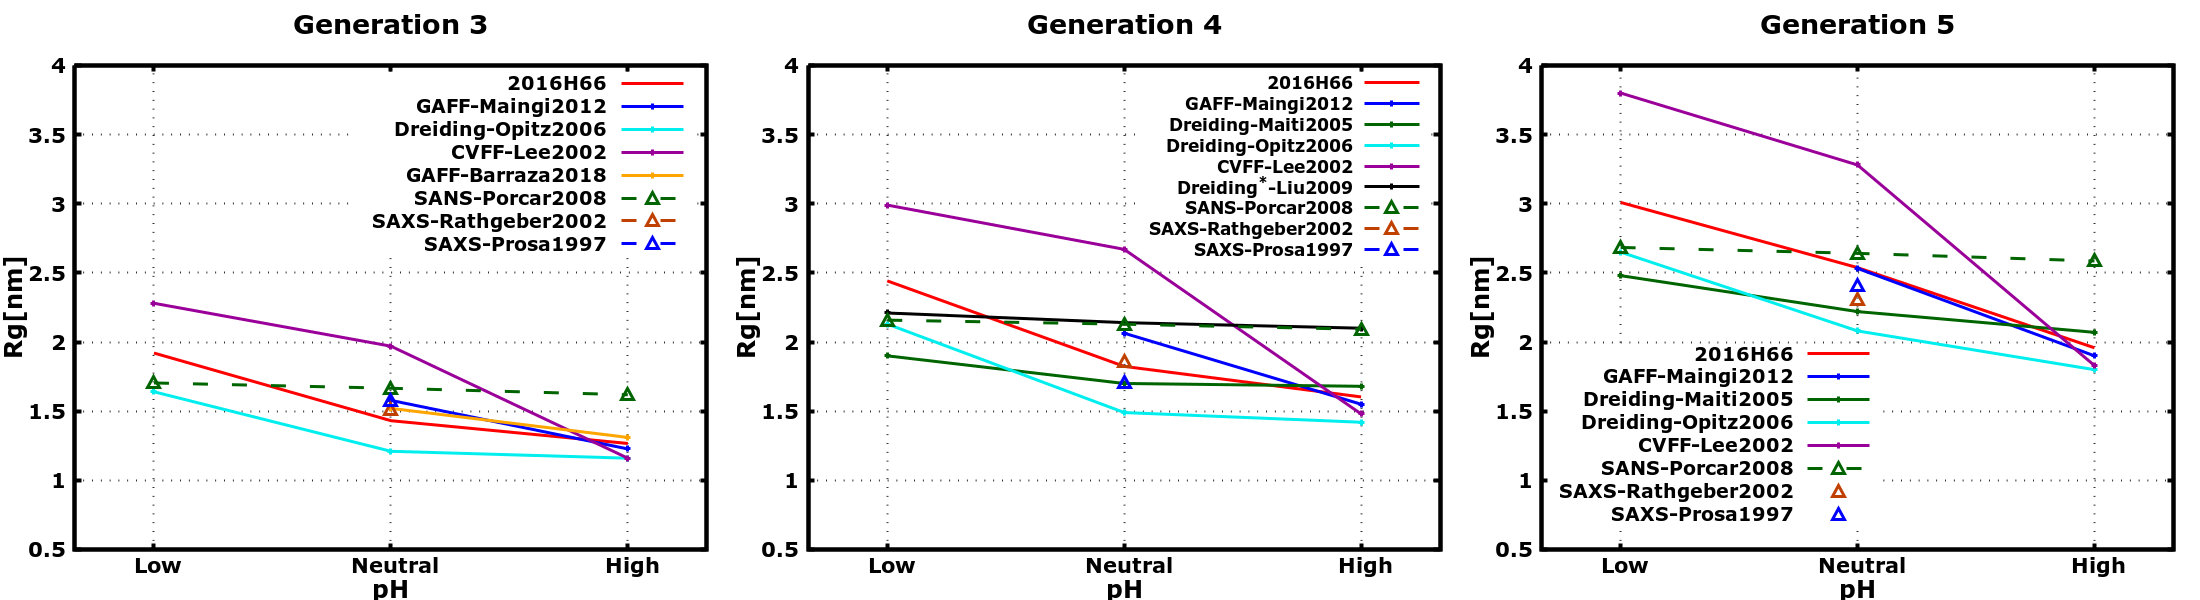
\includegraphics[width=\textwidth]{images/PME/PAMAMgyrateGpH.png}
\caption{Raio de giro ($R_g$) em função do pH para o PAMAM de geração 3 (imagem da esquerda), 4 (imagem do meio) e 5 (imagem da direita).
Os resultados obtidos com o campo de força 2016H66\cite{Horta2016} são comparados com resultados de estudos experimentais e de simulações prévios:
Prosa1997\cite{Prosa1997}, %\cite{PR97.2},
Lee2002\cite{Lee2002}, %\cite{LE02.8},
Rathgeber2002\cite{Rathgeber2002}, %\cite{RA02.6},
Maiti2005\cite{Maiti2005}, %\cite{MA05.26},
Opitz2006\cite{Opitz2006}, %\cite{OP06.1},
Porcar2008\cite{Porcar2008}, %\cite{PO08.3},
Liu2009\cite{Liu2009}, %\cite{LI09.Y},
Maingi2012\cite{Maingi2012}, %\cite{MA12.23}.  }
Barraza2018\cite{Barraza2018}.} %\cite{BA18.Y},
\label{supfig:PAMAMRgpH}   
\end{figure}

\begin{figure*}[ht!]
\centering
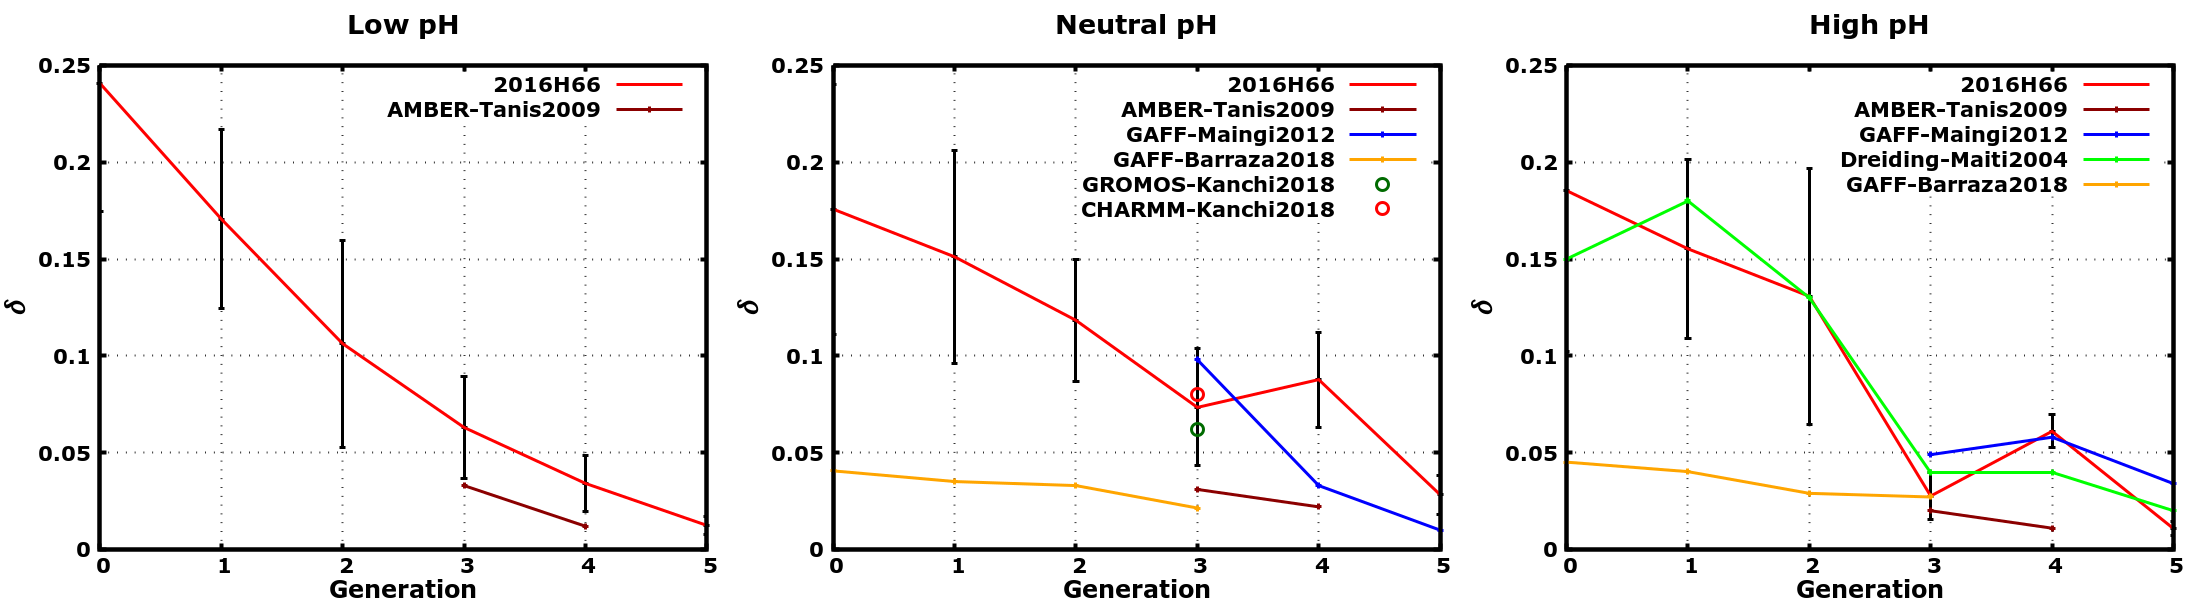
\includegraphics[width=\textwidth]{images/PME/PAMAMAsphericity.png}
\caption{Asfericidade $\delta$ do PAMAM em função da geração. As curvas da esquerda para a direita mostram, respectivamente, os sistemas em baixo, neutro e alto pH.
Os resultados obtidos com o campo de força 2016H66\cite{Horta2016} são comparados com resultados de estudos experimentais e de simulações prévios:
Maiti2004\cite{Maiti2004}, %\cite{MA04.18},
Tanis2009\cite{Tanis2009}, %\cite{TA09.6},
Maingi2012\cite{Maingi2012}, %\cite{MA12.23},
Freire2016\cite{Freire2016}, %\cite{FR16.Y}.}
Barraza2018\cite{Barraza2018}.} %\cite{BA18.Y} and
\label{supfig:PAMAMAsphericity}
\end{figure*}

\begin{figure*}[ht!]
\centering
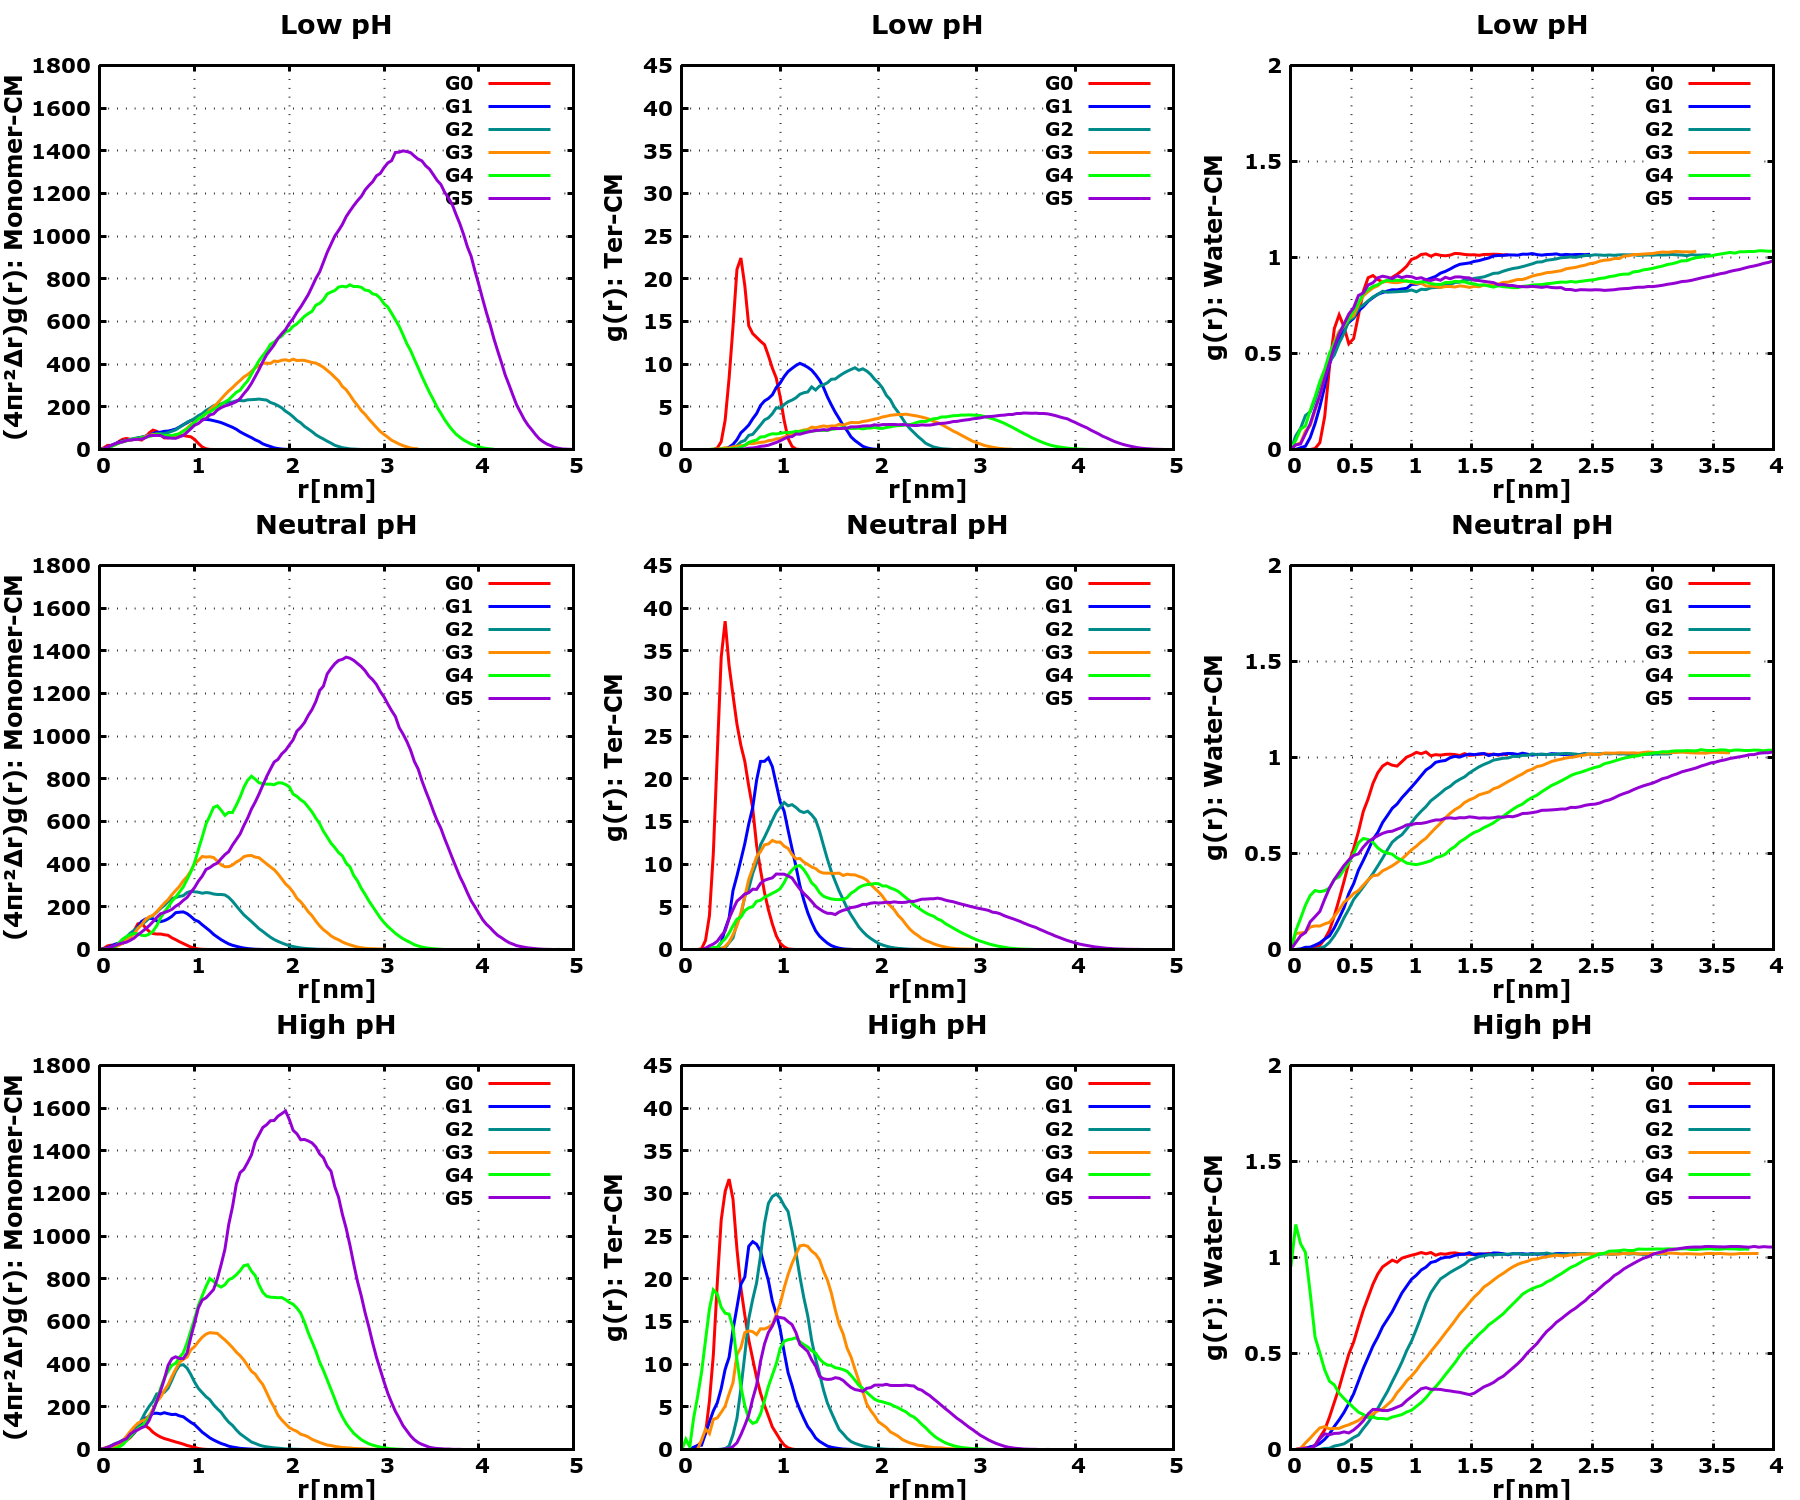
\includegraphics[width=\textwidth]{images/PME/PAMAMRDF.png}
\caption{Função de distribuição radial (RDF) $g(r)$ para o PAMAM. As curvas da esquerda, do meio e da direita mostram, respectivamente, as RDFs do centro de massa do dendrímero em relação à todos os átomos do dendrímero, às aminas primárias terminais e às moléculas de água. E as linhas superiores, intermediárias e inferiores mostram os RDFs descritos anteriormente em condições de pH baixo, neutro e alto, respectivamente. A coluna da esquerda não foi normalizada pelo volume da camada esférica utilizada.}
\label{supfig:PAMAMRDF}
\end{figure*}

\begin{figure*}[ht!]
\centering
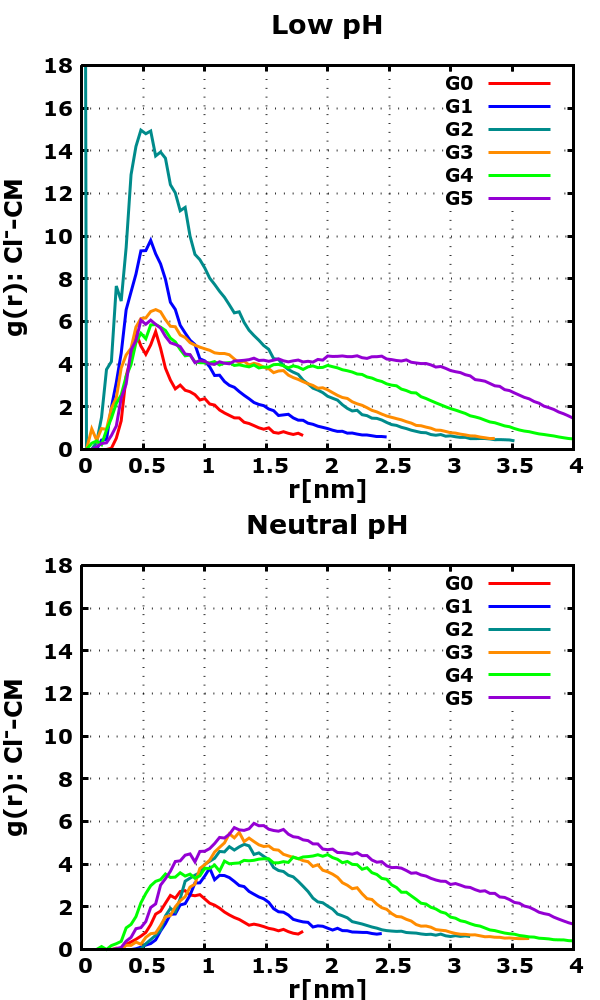
\includegraphics[scale=0.3]{images/PME/PAMAMClRDF.png}
\caption{Função de densidade radial $g(r)$ para o PAMAM. As curvas mostram o RDF de contra-íons Cloreto em relação ao centro de massa do dendrímero para os casos onde o contra-íon está presente(pHs alto e neutro).}
\label{supfig:PAMAMClRDF}
\end{figure*}

\chapter{PPI utilizando o setup PME} \label{PPIap}

\begin{figure*}[ht!]
\centering
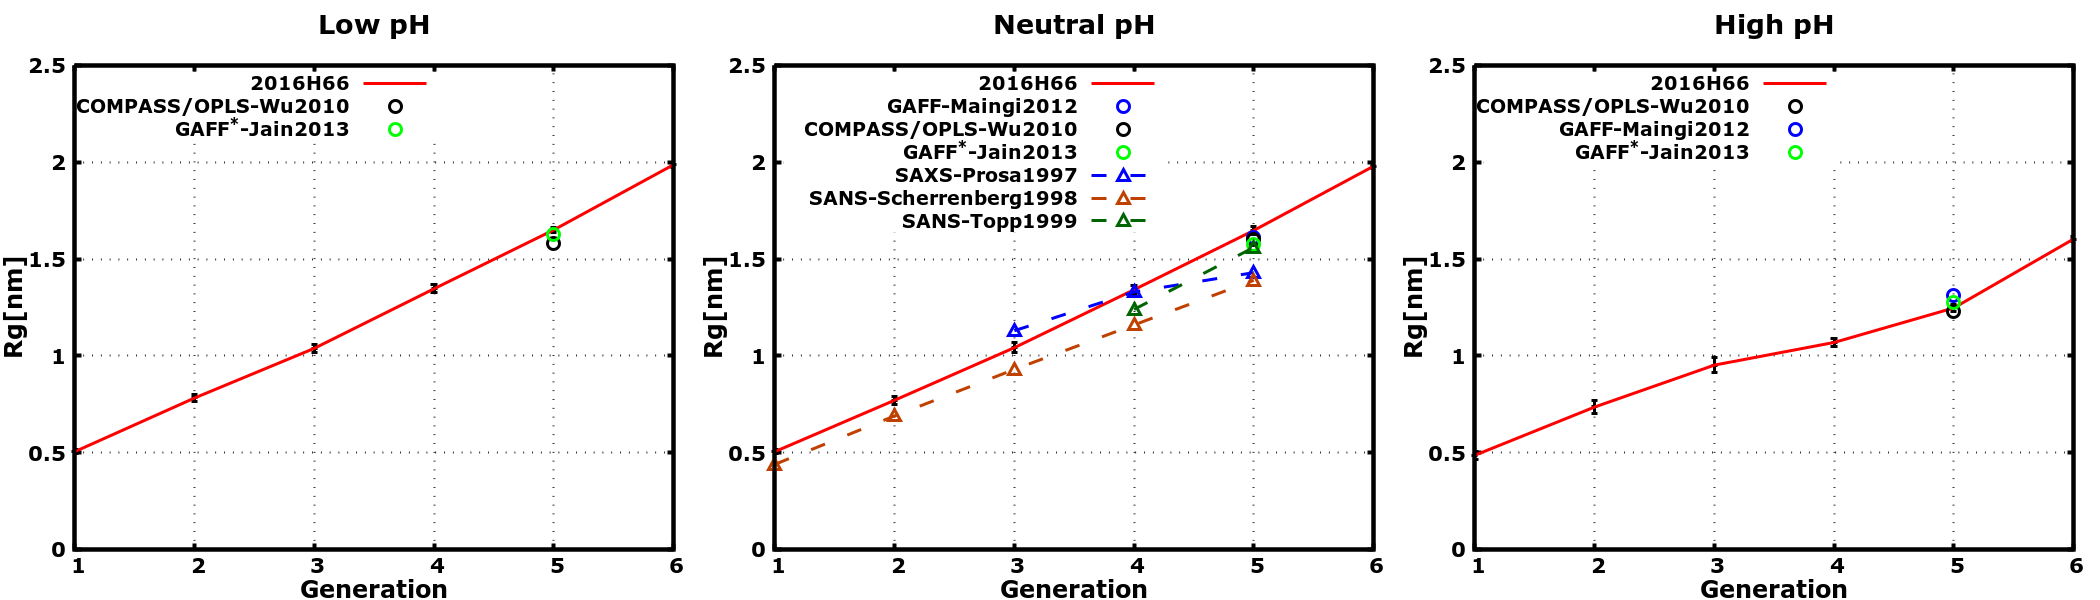
\includegraphics[width=\textwidth]{images/PME/PPIRg.png}
\caption{Raio de giro ($R_g$) em função da geração em meios de pH baixo (curva da esquerda), neutro (curva do meio) e alto (curva da direita).
Os resultados obtidos com o campo de força 2016H66\cite{Horta2016} são comparados com resultados de estudos experimentais e de simulações prévios:
Prosa1997\cite{Prosa1997}, %\cite{PR97.2},
Scherrenberg1998\cite{Scherrenberg1998}, %\cite{SC98.Y},
Topp1999\cite{Topp1999}, %\cite{TO99.Y},
Wu2010\cite{Wu2010}, %\cite{WU10.5},
Maingi2012\cite{Maingi2012}, %\cite{MA12.23},
Jain2013\cite{Jain2013}, %\cite{JA13.4}}
Smeijers2016\cite{Smeijers2016}.} %\cite{SM16.Y}
\label{supfig:PPIRg}
\end{figure*}

\begin{figure*}[ht!]
\centering
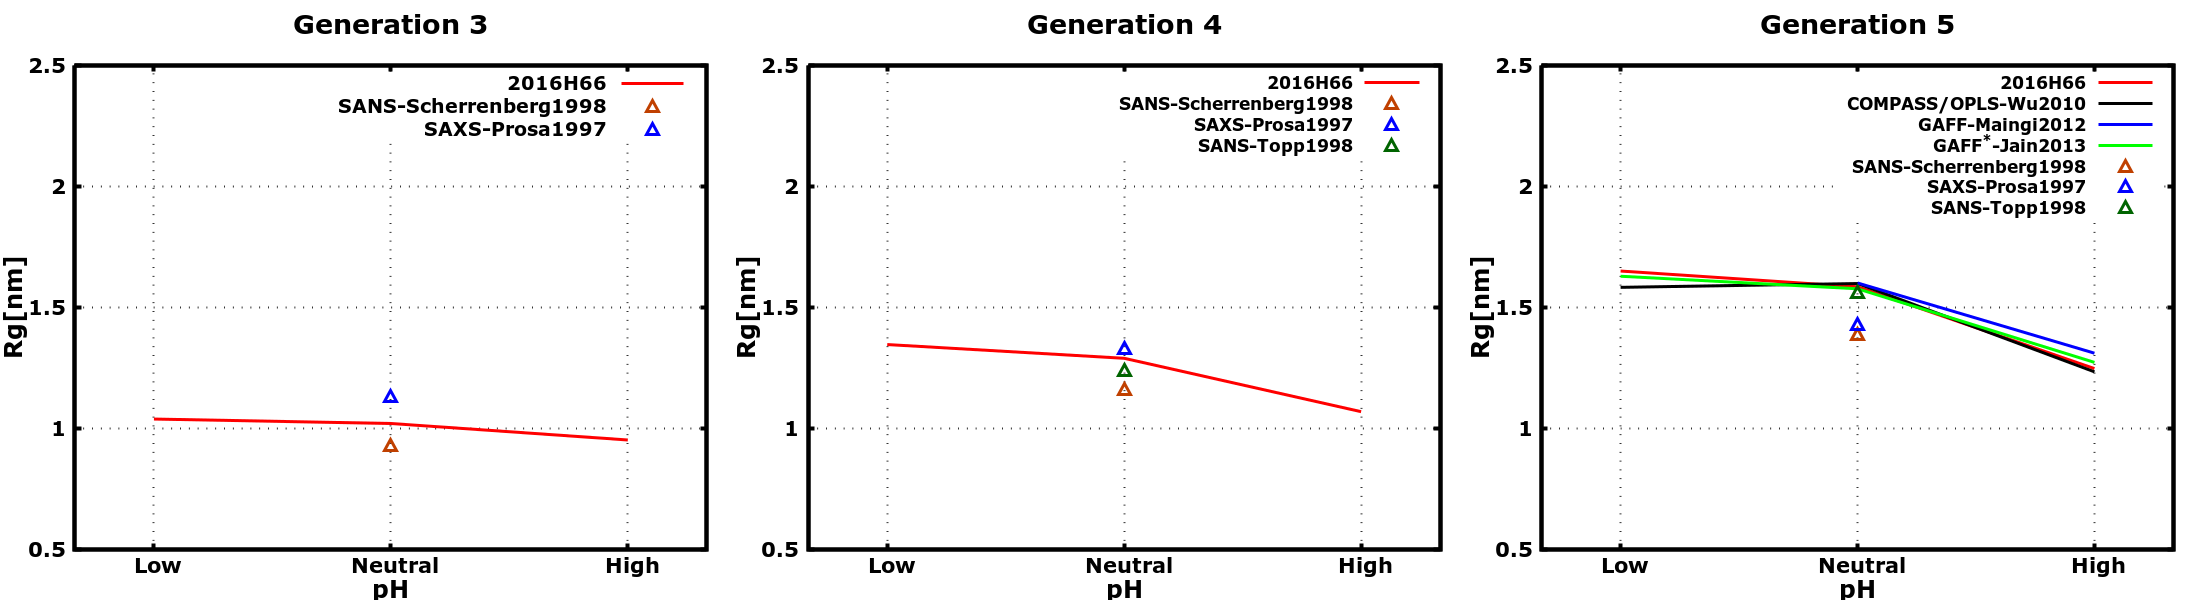
\includegraphics[width=\textwidth]{images/PME/PPIgyrateGpH.png}
\caption{Raio de giro ($R_g$) em função do pH para o PPI de geração 3 (curva da esquerda), 4 (curva do meio) e 5 (curva da direita).
Os resultados obtidos com o campo de força 2016H66\cite{Horta2016} são comparados com resultados de estudos experimentais e de simulações prévios:
Prosa1997\cite{Prosa1997}, %\cite{PR97.2},
Scherrenberg1998\cite{Scherrenberg1998}, %\cite{SC98.Y},
Topp1999\cite{Topp1999}, %\cite{TO99.Y},
Wu2010\cite{Wu2010}, %\cite{WU10.5},
Maingi2012\cite{Maingi2012}, %\cite{MA12.23},
Jain2013\cite{Jain2013}, %\cite{JA13.4}}
Smeijers2016\cite{Smeijers2016}.} %\cite{SM16.Y} and
\label{supfig:PPIRgpH}
\end{figure*}

\begin{figure*}[ht!]
\centering
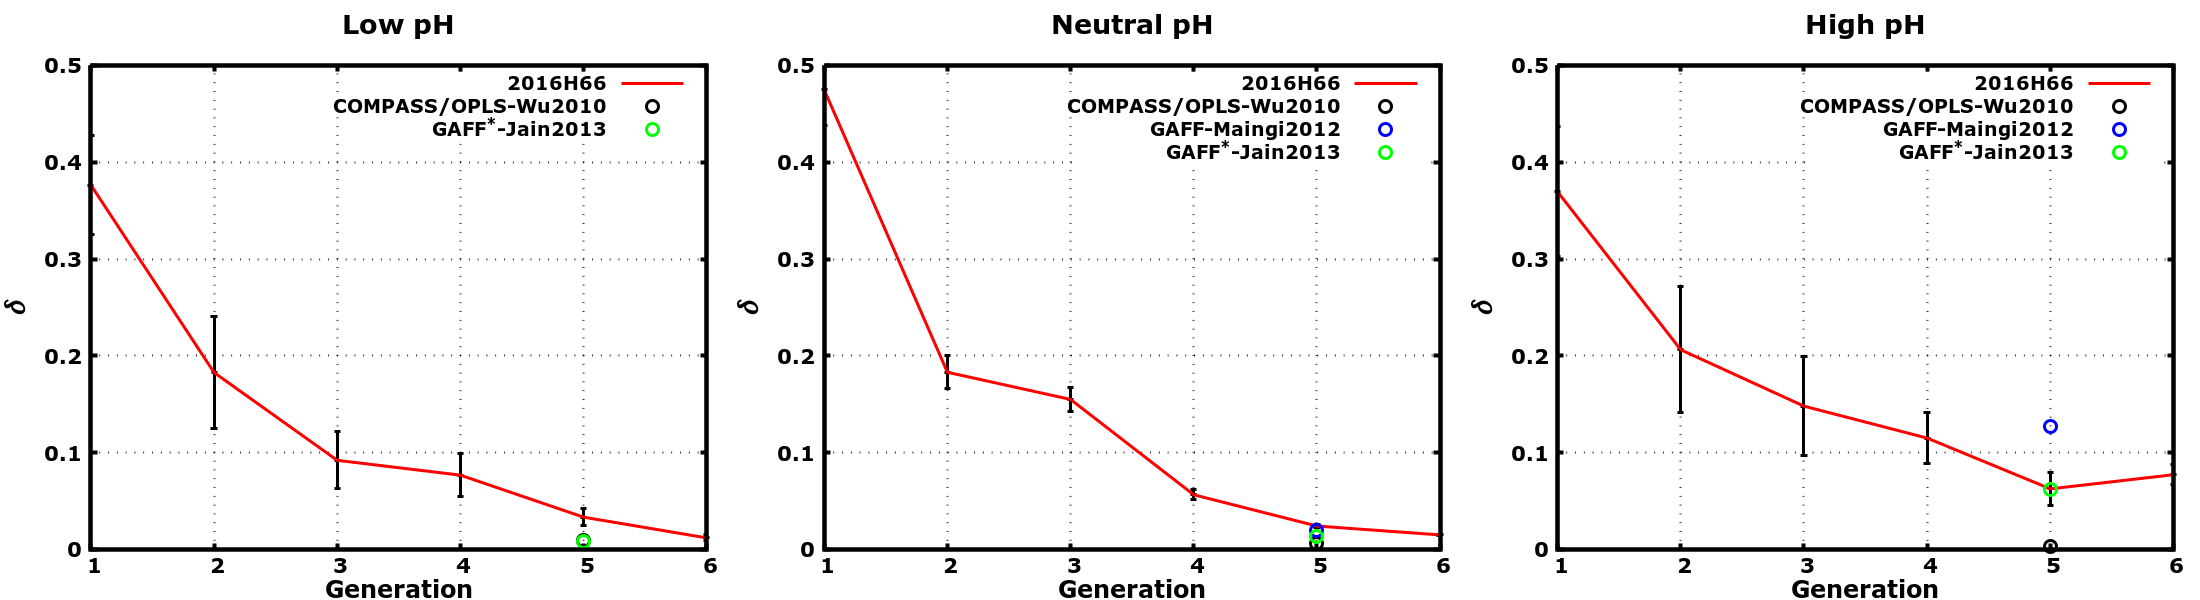
\includegraphics[width=\textwidth]{images/PME/PPIAsphericity.png}
\caption{Asfericidade $\delta$ do PPI em função da geração. As curvas da esqueda para a direita mostram os sistemas em baixo, neutro e alto pH, respectivamente.
Os resultados obtidos com o campo de força 2016H66\cite{Horta2016} são comparados com resultados de estudos experimentais e de simulações prévios:
Wu2010\cite{Wu2010}, %\cite{WU10.5}, 
Maingi2012\cite{Maingi2012}, %\cite{MA12.23}, 
Jain2013\cite{Jain2013}.} %\cite{JA13.4}}
\label{supfig:PPIAsphericity}
\end{figure*}

\begin{figure}[ht!]
\centering
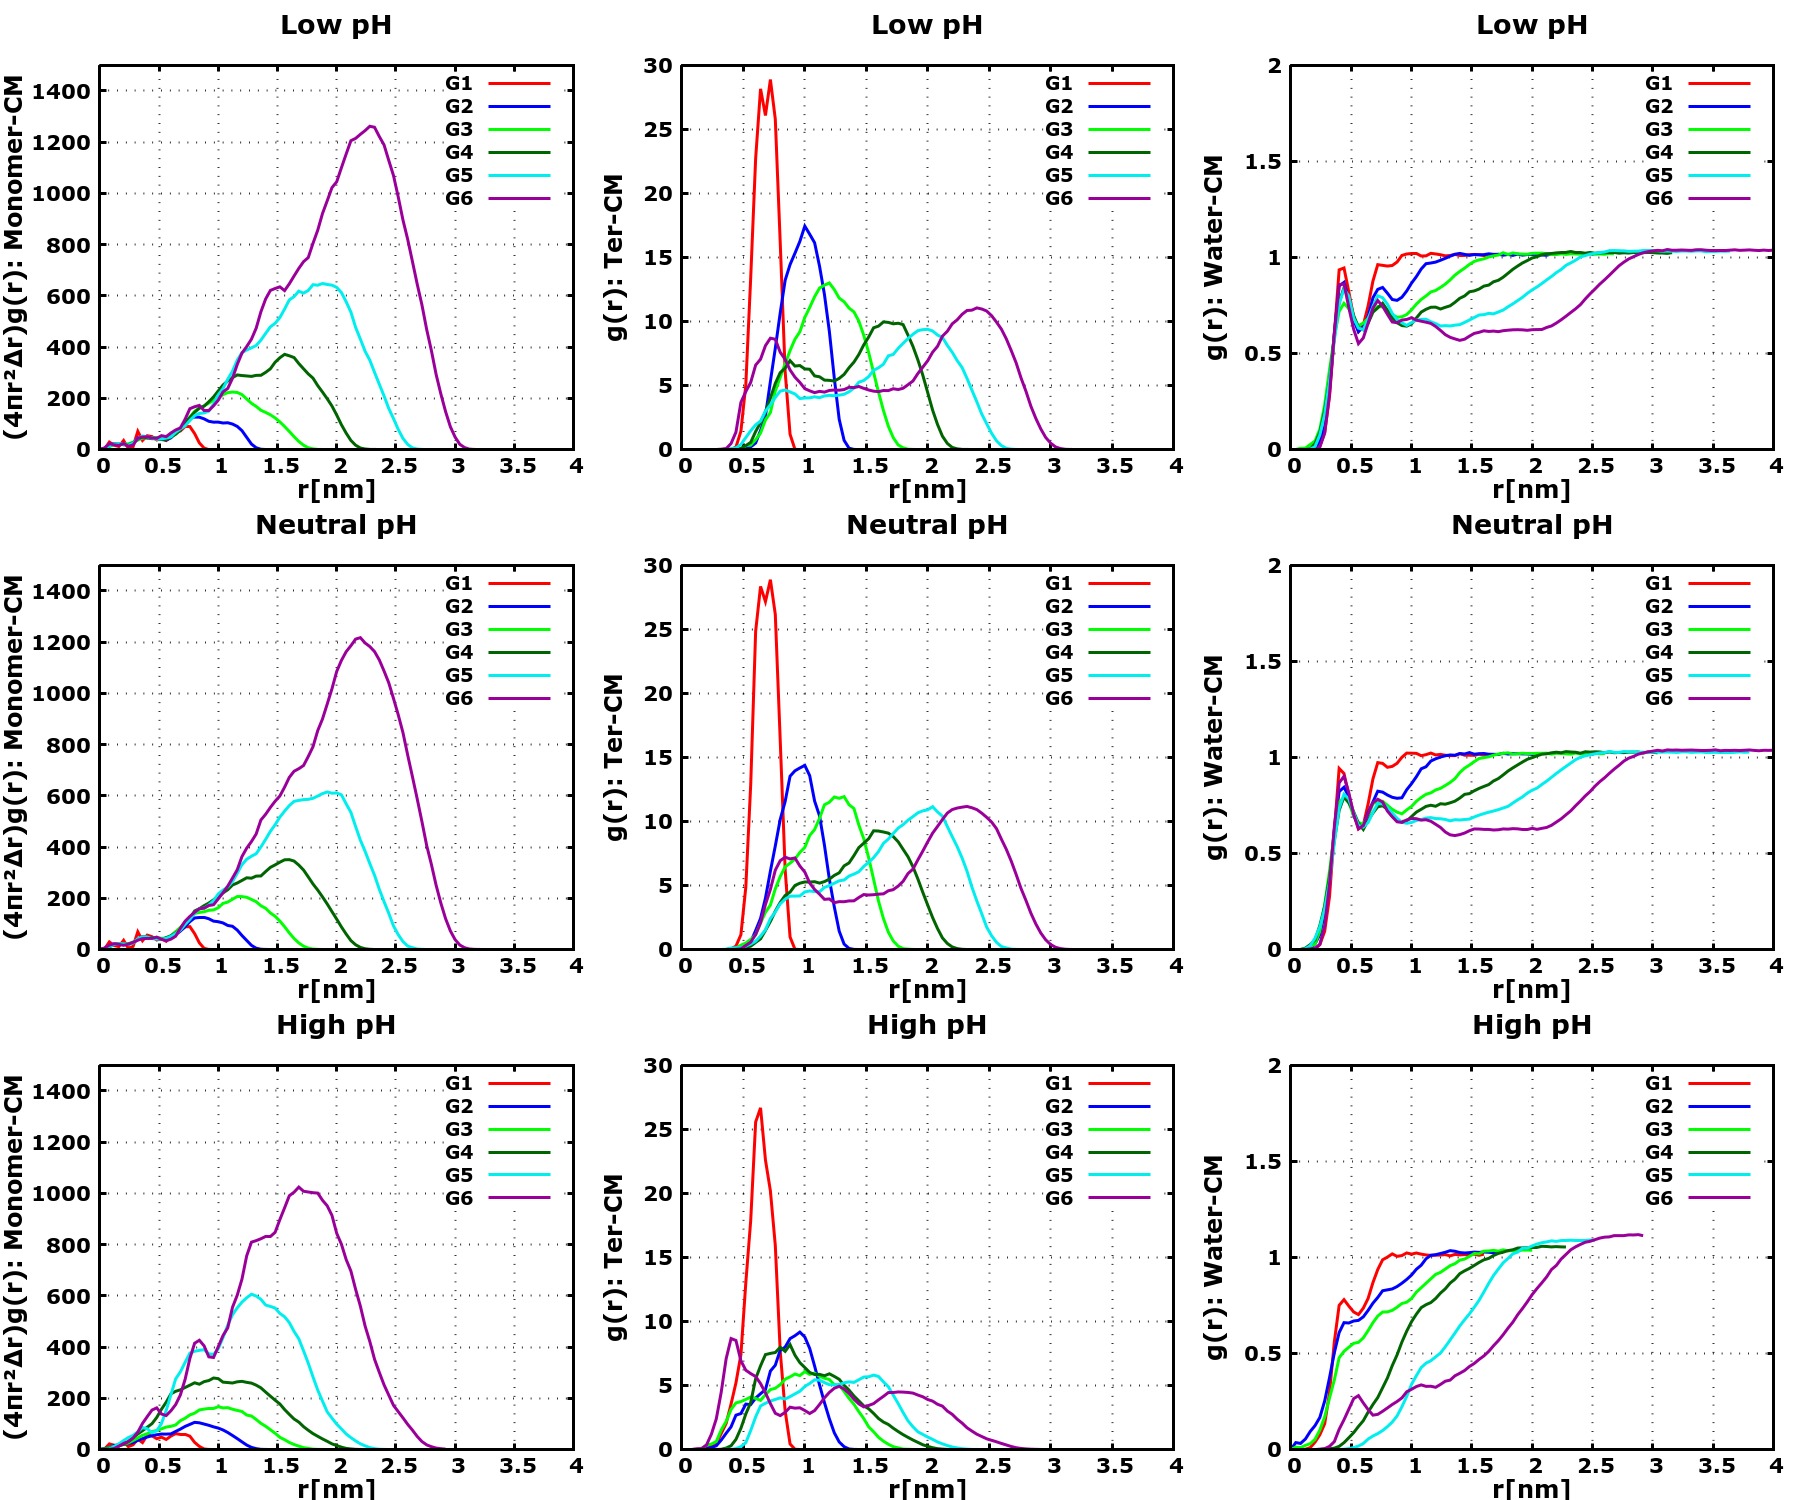
\includegraphics[width=\textwidth]{images/PME/PPIRDF.png}
\caption{Função de distribuição radial (RDF) $g(r)$ para o PAMAM. As curvas da esquerda, do meio e da direita mostram, respectivamente, as RDFs do centro de massa do dendrímero em relação à todos os átomos do dendrímero, às aminas primárias terminais e às moléculas de água. E as linhas superiores, intermediárias e inferiores mostram os RDFs descritos anteriormente em condições de pH baixo, neutro e alto, respectivamente. A coluna da esquerda não foi normalizada pelo volume da camada esférica utilizada.}
\label{supfig:PPIRDF}
\end{figure}

\begin{figure}[ht!]
\centering
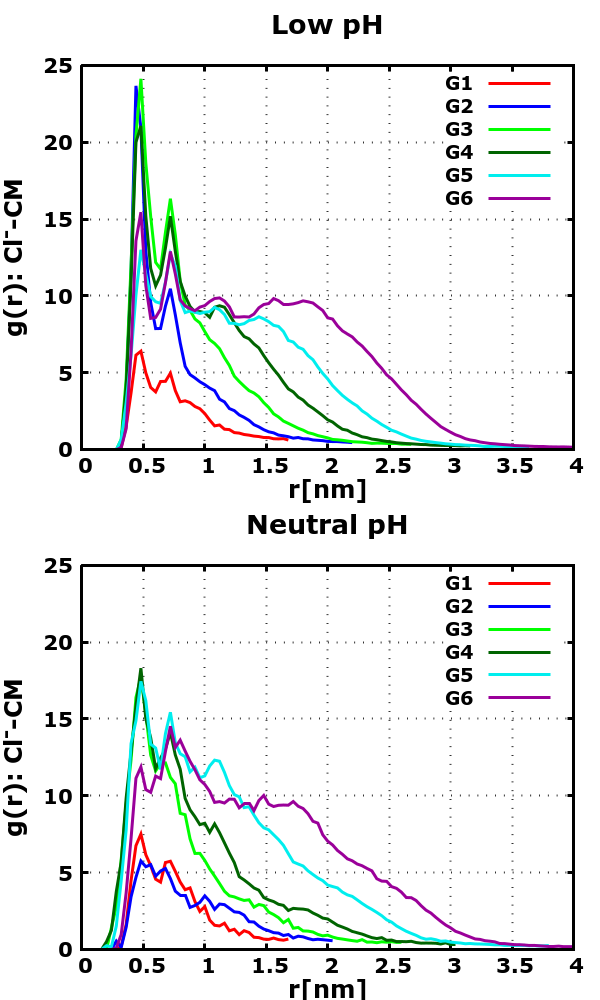
\includegraphics[scale=0.3]{images/PME/PPIClRDF.png}
\caption{Função de distribuição radial g(r) para o PPI. As curvas mostram o RDF de contra-íons cloreto em relação ao centro de massa do dendrímero para os casos onde o contra-íon está presente(pHs alto e neutro).}
\label{supfig:PPIClRDF}
\end{figure}

% ----------------------------------------------------------


\end{apendicesenv}
% ---


% ----------------------------------------------------------
% Anexos
% ----------------------------------------------------------

%\begin{anexosenv}

% Imprime uma página indicando o início dos anexos
%\partanexos

% ---
%\chapter{Morbi ultrices rutrum lorem.}
% ---


%\end{anexosenv}

%---------------------------------------------------------------------
% INDICE REMISSIVO
%---------------------------------------------------------------------
\phantompart
\printindex
%---------------------------------------------------------------------

\end{document}
\grid